\documentclass[pdflatex,sn-mathphys-ay]{sn-jnl}

\usepackage[utf8]{inputenc}%
\usepackage[T1,T2A]{fontenc}%
\usepackage[english,russian]{babel}%
\usepackage{graphicx}%
\usepackage{multirow}%
\usepackage{amsmath,amssymb,amsfonts}%
\usepackage{amsthm}%
\usepackage{mathrsfs}%
\usepackage[title]{appendix}%
\usepackage{xcolor}%
\usepackage{textcomp}%
\usepackage{manyfoot}%
\usepackage{booktabs}%
\usepackage{array}%
\usepackage{longtable}%
\usepackage{calc}%
\usepackage{newunicodechar}%
\usepackage{fvextra}%
\providecommand{\tightlist}{\setlength{\itemsep}{0pt}\setlength{\parskip}{0pt}}
\providecommand{\lt}{<}\providecommand{\gt}{>}
\newunicodechar{§}{\S}
\newunicodechar{→}{\ensuremath{\rightarrow}}
\newunicodechar{↔}{\ensuremath{\leftrightarrow}}
\newunicodechar{×}{\ensuremath{\times}}
\newunicodechar{·}{\ensuremath{\cdot}}
\newunicodechar{⊃}{\ensuremath{\supset}}
\newunicodechar{°}{\ensuremath{^{\circ}}}
\newunicodechar{₀}{\textsubscript{0}}\newunicodechar{₁}{\textsubscript{1}}%
\newunicodechar{₂}{\textsubscript{2}}\newunicodechar{₃}{\textsubscript{3}}%
\newunicodechar{₄}{\textsubscript{4}}\newunicodechar{₅}{\textsubscript{5}}%
\newunicodechar{₆}{\textsubscript{6}}\newunicodechar{₇}{\textsubscript{7}}%
\newunicodechar{₈}{\textsubscript{8}}\newunicodechar{₉}{\textsubscript{9}}%
\newunicodechar{⁰}{\textsuperscript{0}}\newunicodechar{¹}{\textsuperscript{1}}%
\newunicodechar{²}{\textsuperscript{2}}\newunicodechar{³}{\textsuperscript{3}}%
\newunicodechar{⁴}{\textsuperscript{4}}\newunicodechar{⁵}{\textsuperscript{5}}%
\newunicodechar{⁶}{\textsuperscript{6}}\newunicodechar{⁷}{\textsuperscript{7}}%
\newunicodechar{⁸}{\textsuperscript{8}}\newunicodechar{⁹}{\textsuperscript{9}}%
\newunicodechar{⁻}{\textsuperscript{-}}\newunicodechar{≈}{\ensuremath{\approx}}%
\newunicodechar{≤}{\ensuremath{\le}}\newunicodechar{≥}{\ensuremath{\ge}}%
\newunicodechar{∼}{\ensuremath{\sim}}\newunicodechar{−}{\ensuremath{-}}%
\newunicodechar{∗}{\ensuremath{\ast}}\newunicodechar{∞}{\ensuremath{\infty}}%
\newunicodechar{τ}{\ensuremath{\tau}}\newunicodechar{ν}{\ensuremath{\nu}}%
\newunicodechar{λ}{\ensuremath{\lambda}}\newunicodechar{σ}{\ensuremath{\sigma}}%
\newunicodechar{α}{\ensuremath{\alpha}}\newunicodechar{η}{\ensuremath{\eta}}%
\newunicodechar{π}{\ensuremath{\pi}}\newunicodechar{μ}{\ensuremath{\mu}}\newunicodechar{ρ}{\ensuremath{\rho}}%
\newunicodechar{θ}{\ensuremath{\theta}}\newunicodechar{β}{\ensuremath{\beta}}\newunicodechar{γ}{\ensuremath{\gamma}}%
\newunicodechar{δ}{\ensuremath{\delta}}\newunicodechar{ε}{\ensuremath{\varepsilon}}\newunicodechar{κ}{\ensuremath{\kappa}}%
\newunicodechar{ξ}{\ensuremath{\xi}}\newunicodechar{ω}{\ensuremath{\omega}}\newunicodechar{χ}{\ensuremath{\chi}}%
\newunicodechar{ψ}{\ensuremath{\psi}}\newunicodechar{φ}{\ensuremath{\varphi}}\newunicodechar{Δ}{\ensuremath{\Delta}}%
\newunicodechar{Σ}{\ensuremath{\Sigma}}\newunicodechar{Π}{\ensuremath{\Pi}}\newunicodechar{Ω}{\ensuremath{\Omega}}%
\newunicodechar{Γ}{\ensuremath{\Gamma}}\newunicodechar{Λ}{\ensuremath{\Lambda}}\newunicodechar{Θ}{\ensuremath{\Theta}}%
\newunicodechar{«}{\guillemotleft}
\newunicodechar{»}{\guillemotright}

\raggedbottom

\begin{document}

\title[Информационная ностальгия]{Информационная ностальгия: рост памяти, неустранимый недобор прогноза и термодинамика нестационарного обучения}

\author*[1]{\fnm{Александр} \sur{Андриишин}}\email{alexander@andriishin.com}

\affil*[1]{\orgname{Independent Researcher}, \orgaddress{\city{Москва}, \country{Россия}}}

\abstract{Активно удерживаемая память --- не запись, а термодинамический процесс, оплачивающий себя. Бактерия удерживает память о концентрации лиганда через метилирование рецепторов; эмбрион млекопитающего стирает эпигенетическое прошлое массивным перепрограммированием; нейросеть в режиме continual learning расходует энергию на обновление весов; биосферы копят в геномах летопись исчезнувшей среды. Во всех этих системах память поддерживается против среды, которая дрейфует быстрее темпа её обновления, и растущая доля хранимых битов уже ничего не предсказывает. Мы называем эту долю \emph{информационной ностальгией} (технический термин, не психологический референт) и измеряем её \emph{недобором прогноза} --- долей предсказуемого будущего среды, которую система упускает. Рамка применима при методологическом условии самооплаты: каждый удерживаемый бит оплачивается собственной свободной энергией системы, а термодинамическую цену удержания даёт отдельный бонд Still. Доказываются два результата. \emph{Лемма 1}: удержание каждого бита против термодинамической эрозии требует строго положительной мощности с явной нижней оценкой. \emph{Лемма 2} (условный результат для своего класса): при любом конечном темпе обновления и медленном гауссовском дрейфе среды с экспоненциально затухающей корреляцией недобор прогноза не падает ниже явной положительной константы --- при проверяемом численно допущении об аддитивности; устаревание памяти в этом классе неизбежно. Отсюда: без достаточного забывания предсказательная способность коллапсирует (подтверждено численно на марковских цепях с дрейфом), и существует оптимальный темп сброса устаревшего слоя памяти, созвучный эпигенетическому перепрограммированию. Рамка помещает bet-hedging, active inference и catastrophic forgetting на общую шкалу ностальгии. Для хемотаксиса \emph{E. coli} формулируется pre-registration-ready \emph{количественное} предсказание --- пол недобора, отличающий рамку от стандартной кинетики адаптации. Стационарный случай развит в сопровождающей работе (Andriishin 2026) и восстанавливается здесь как предельный.}

\keywords{informational nostalgia, vitality, self-payment, non-stationary thermodynamics, predictive information, active inference}

\maketitle

\section{Введение}\label{ux432ux432ux435ux434ux435ux43dux438ux435}



\emph{Хемотаксис E. coli как мотивирующий пример.} Бактерия \emph{Escherichia coli} плывёт вверх по градиенту аспартата, удерживая память о концентрации лиганда минуту назад через ковалентное метилирование четырёх остатков Tar/Tsr-рецепторов (Sourjik and Berg 2002). Метилтрансфераза CheR добавляет метильные метки, метилэстераза CheB их удаляет; равновесие между ними --- это и есть «память» о недавнем градиенте, переводимая в bias тумблинга. Характерное время обновления этих меток --- порядка минуты, время отклика --- десятки секунд. Когда источник аспартата резко перемещается, метильные метки обновляются медленнее, чем подвинулся градиент: часть конфигурации рецепторов кодирует уже не существующую среду. Эта \emph{устаревшая фракция памяти} продолжает стоить бактерии ATP (поддержание метилтрансферазной активности, репарация деградировавших меток), но не помогает предсказывать локальный градиент сейчас. Что сенсорная адаптация в этой системе сопряжена с энергетической ценой --- установленный факт: граница энергия--скорость--точность для адаптации хемотаксиса (Lan et al.~2012) и общая энергетика клеточного вычисления (Mehta and Schwab 2012) показали, что точность и темп адаптации оплачиваются диссипацией. Адаптация догоняет --- но не мгновенно; лаг между сдвигом среды и сдвигом памяти физически дорог. Отсюда конкретный фальсифицируемый исход: бактерия с пониженной активностью метилтрансферазы CheR (\(cheR^{\downarrow}\), замедленный темп обновления меток) под периодической сменой концентрации аттрактанта должна \emph{медленнее} восстанавливать адаптацию, чем дикий тип, --- измеримое замедление adaptation rate на стандартном лабораторном протоколе (§ 8.6, Предсказание 2).



\emph{Та же структура повторяется на разных масштабах.} Биосферы накапливают геномное содержание через эволюционные переходы (Maynard Smith and Szathmáry 1995; Landenmark et al.~2015); абиотические циклы сменяются на эоновых окнах, оставляя в геномах летопись прошлых режимов. Популяции в флуктуирующих средах поддерживают фенотипическое разнообразие как информационную ставку на возможные будущие состояния (Kussell and Leibler 2005) --- bet-hedging описывает ту же асимметрию между темпом обновления распределения фенотипов и темпом сдвига среды. У млекопитающих в раннем эмбриогенезе происходит почти полное стирание метилирования ДНК с повторной установкой (Reik 2007) --- массивный сброс устаревшей эпигенетической памяти. Нейросети под continual learning демонстрируют \emph{catastrophic forgetting} (McCloskey and Cohen 1989; Kirkpatrick et al.~2017); крупные языковые модели с замороженными весами после обучения накапливают всё больше параметров, описывающих лексику и факты, актуальные на момент отсечки, но дрейфующие с потоком новых данных (Lazaridou et al.~2021). Все эти системы объединяет структурная аналогия (не эквивалентность): память о прошлом состоянии среды растёт, среда дрейфует на тех же временах, а оптимальная стратегия удержания памяти балансирует информационный выигрыш против термодинамической цены. Количественная мера этого баланса --- открытый вопрос на стыке стохастической термодинамики, популяционной биологии и теории обучения.



\emph{Мера баланса.} Чтобы измерить этот баланс, нужна одна безразмерная величина, сопоставляющая \emph{предсказательную} часть удерживаемой памяти со всей удерживаемой памятью. Вернёмся к бактерии: пока метильные метки успевают за градиентом, почти вся удерживаемая память ещё предсказывает ближайшее будущее среды --- она полезна; когда источник аспартата уходит быстрее, чем обновляются метки, растущая доля памяти кодирует уже несуществующую среду и перестаёт что-либо предсказывать --- это балласт. Эту растущую непредсказательную долю памяти мы называем \emph{информационной ностальгией} (технический термин, не психологический референт). Её \emph{операционально ведущая} мера --- \emph{недобор прогноза} \(\nu^{\text{op}}\) (индекс op --- операциональный): доля предсказуемого будущего среды, которую система упускает; у мутанта \(cheR^{\downarrow}\) с замедленным обновлением меток рамка предсказывает его выше, чем у дикого типа (проверяемое следствие, § 8.6 П.2). Строгое определение и вся семья из четырёх нормировок одной и той же ностальгии --- § 4.1.



Формализация опирается на две информационные величины. Пусть \(M_t\) --- конфигурация тех внутренних степеней свободы системы \(X\), что принадлежат моделирующему контуру (функциональный канал: для \emph{E. coli} --- паттерн метилирования Tar/Tsr-рецепторов, не все \(\sim 10^{10}\) степеней свободы клетки), а \(X_E\) --- сигнал её среды. В духе Still, Sivak, Bell, Crooks (2012) вводятся



\[I_{\text{mem}}(t) := I\!\left(M_t;\, X_E^{\le t}\right), \qquad I_{\text{pred}}(t,\tau) := I\!\left(M_t;\, X_E^{[t,\,t+\tau]}\right),\]



где \(I_{\text{mem}}(t)\) --- \textbf{память} (сколько внутреннее состояние знает о прошлой и текущей траектории среды), а \(I_{\text{pred}}(t,\tau)\) --- \textbf{предсказательная информация} (Bialek et al.~2001; Tishby et al.~1999), часть этого знания, относящаяся к будущему среды на горизонте \(\tau\). Здесь \(M_t\) --- актуальный слой моделирующего контура, и обе величины даны в \emph{концептуальной форме}: центральная \emph{растущая} память формализуется на полной памяти \(M_{\le t}\) как \(I_{\text{mem}}(t) = I(M_{\le t}; X_E^{\le t})\) (§ 2.1, § 3.1), а операциональная одношаговая версия \(I_{\text{pred}}\) --- формула (4) § 3.1. Отсюда пара сопряжённых величин ---



\begin{equation}\eta_v(t) = \frac{I_{\text{pred}}(t,\tau)}{I_{\text{mem}}(t)} = 1 - \nu(t), \qquad \nu(t) := \frac{I_{\text{mem}}(t) - I_{\text{pred}}(t,\tau)}{I_{\text{mem}}(t)}, \tag{1}\end{equation}



где \(\nu(t) = 1 - \eta_v\) --- балластная нормировка \emph{информационной ностальгии}: доля удерживаемой памяти, переставшая быть предсказательной. Её дополнение \(\eta_v(t) = I_{\text{pred}}/I_{\text{mem}}\) --- \emph{предсказательная эффективность самомоделирования} (самомоделирование --- удержание системой внутренней модели своей среды; индекс v --- vitality; доля удержанного, ещё предсказывающая среду): вторичный структурно-термодинамический индекс, наследуемый из статьи-предшественницы. Он несёт термодинамический бонд Still --- нижнюю термодинамическую границу (bound) Still 2012: диссипация \(\ge k_B T\cdot\)(память \(-\) предсказание), § 2.2 --- и служит мостом к стационарному случаю статьи \#1. Различие \emph{концептуального} и \emph{операционального} числителя \(I_{\text{pred}}\) и статус верхней границы \(\eta_v \le 1\) (для концептуального --- теорема из неравенства об обработке данных, DPI; для операционального --- следствие нормировки и конечно-выборочного усечения) разъяснены в § 3.1.



\emph{Нестационарность --- в знаменателе-информации.} Специфика настоящей работы в том, что \(I_{\text{mem}}(t)\) \textbf{растёт} по мере накопления памяти, тогда как \(I_{\text{pred}}(t,\tau)\) ограничена горизонтом предсказания и скоростью энтропии среды. Поэтому при дрейфующей среде и конечном темпе обновления памяти \(\eta_v(t) \to 0\), \(\nu(t) \to 1\): система накапливает всё больше непредсказательной памяти. Механизм здесь \textbf{информационный}: он следует из роста \emph{информационного} знаменателя \(I_{\text{mem}}(t)\) при ограниченном горизонтом \(I_{\text{pred}}\). Стационарный случай (Andriishin 2026) --- частный предел \(\dot I_{\text{mem}} \to 0\), в котором \(\eta_v\) выходит на постоянный уровень (§ 2.5).



\emph{Несущий результат и что здесь лишь постановка.} Главный результат работы формулируется просто: даже при \emph{фиксированной} ёмкости памяти дрейф среды и конечный темп обновления оставляют неустранимый \emph{недобор прогноза} --- \(\nu^{\text{theor}} \ge 1 - c > 0\) (Лемма 2, § 4.4; строгие и измеримые версии меры разведены в § 4.1). Именно он разделяет адаптацию и коллапс; его динамика показана на рисунках § 6. Его важно отличать от более простого структурного эффекта --- падения \(\eta_v(t) \to 0\) по мере роста \(I_{\text{mem}}(t)\): оно наступает при любом накоплении памяти и режимы \emph{не различает}, а потому есть постановка задачи, не результат. Обе грани измеряют одну ностальгию разными нормировками; их полное разведение и роли --- § 4.1.



\emph{Термодинамический якорь --- отдельная линия.} Удержание непредсказательной памяти не бесплатно. Still et al.~(2012) доказывают точную нижнюю цену этого балласта: на каждом шаге обновления памяти диссипация ограничена снизу \(\langle W_{\text{diss}}\rangle \ge k_B T\,(I_{\text{mem}}^{\text{инст}} - I_{\text{pred}}^{\text{инст}})\), а кумулятивно --- суммой пошаговых вкладов (§ 2.2). Эта граница --- \textbf{отдельный термодинамический якорь}: \(k_B T\) входит как коэффициент границы из теоремы, а энергетика удержания и роста памяти учитывается этим полом на диссипацию (детали --- § 2.2), дополняющим информационную границу \(\eta_v \le 1\).



\emph{Постулат самооплаты.} Отношение \(\eta_v\) применимо к физической системе, когда числитель и знаменатель принадлежат одному \emph{контуру самооплаты}: система сама расходует собственную свободную энергию на удержание своей модели против термодинамической эрозии, а не получает её извне (§ 2.7). Операциональный тест --- counterfactual ablation (отключение метаболической подпитки и проверка деградации памяти за время отклика \(\tau_d\)).



\emph{Содержание работы.} Устанавливаются три структурных результата с интуитивной интерпретацией:



\begin{itemize}

\tightlist

\item

  \textbf{Лемма 1} (§ 2.3) --- удержание каждого непредсказательного бита против термодинамической эрозии требует строго положительной мощности с явной нижней оценкой (термодинамический пол бонда Still; для naive-refresh (слепое переписывание бита без проверки) --- полиномиальная по порогу ошибки \(\varepsilon\) форма (3), для feedback-памяти (переписывание с проверкой ошибки, как в коррекции ошибок) --- логарифмическая (3')).

\item

  \textbf{Лемма 2} (§ 4.4) --- при медленном OU-дрейфе среды (Орнштейна--Уленбека; канонический класс «медленного дрейфа среды», § 5.2) и конечном темпе обновления \(\dot M_{\text{refresh}}\) ностальгическая фракция \(\nu(t)\) асимптотически не падает ниже \(1 - c\), где \(c = \dot M_{\text{refresh}}\, \tau_E / \lvert M_{\le t}\rvert\) (\(\tau_E\) --- время корреляции среды) --- явная вычислимая константа.

\item

  \textbf{Критический уровень ностальгии \(\nu_c\)} (§ 5.3) --- порог, выше которого эффективность практически обращается в ноль; и \textbf{оптимальный сброс \(\tau_{\text{reset}}^*\)} (§ 5.3) --- оптимальная частота полного сброса памяти (эпигенетическое перепрограммирование раннего эмбриогенеза, Reik 2007; диапаузы \emph{Daphnia}).

\end{itemize}



\emph{Отличие от смежных рамок.} Параллели с bet-hedging (ставка-страховка на несколько возможных сред), catastrophic forgetting (забывание старого при дообучении новому) и concept drift (дрейф распределения данных во времени) --- структурные, не эквивалентные: новое здесь --- общая шкала, на которой предсказательная часть памяти сопоставляется со всей удерживаемой памятью одной физической системы, и нижняя граница неизбежной ностальгии (Лемма 2). Подробное сопоставление --- § 8.4.



\emph{Отстройка от термодинамики предсказания и обучения.} Ближайшая линия работ --- эффективность обучения Голдт--Зайферта (Goldt and Seifert 2017) и КПД приобретения структуры среды Такахаси--Хаяси (Takahashi and Hayashi 2026) --- делит с нами общий фундамент (Landauer 1961; Still et al.~2012), но отличается предметом: те работы меряют, как система \emph{набирает} информацию о среде, тогда как информационная ностальгия (недобор прогноза) --- как уже удержанное \emph{устаревает}. Настоящая работа делает эту цену удержания центральной; развёрнутое сопоставление --- § 8.4, линии комплементарны.



\emph{Структура работы.} § 2 --- нестационарная предсказательная эффективность, термодинамический якорь и self-payment, глоссарий ключевых обозначений (§ 2.0); § 3 --- predictive information на растущей памяти; § 4 --- ностальгия и Лемма 2; § 5 --- \(\eta_v(t)\), три режима, режимный порог \(\nu_c\), оптимальный \(\tau_{\text{reset}}^*\); § 6 --- численная иллюстрация; § 7 --- связь с active inference (активным выводом); § 8 --- итоги, прикладные следствия, открытые проблемы.



\section{Ностальгия, предсказательная эффективность и термодинамический якорь}\label{ux43dux43eux441ux442ux430ux43bux44cux433ux438ux44f-ux43fux440ux435ux434ux441ux43aux430ux437ux430ux442ux435ux43bux44cux43dux430ux44f-ux44dux444ux444ux435ux43aux442ux438ux432ux43dux43eux441ux442ux44c-ux438-ux442ux435ux440ux43cux43eux434ux438ux43dux430ux43cux438ux447ux435ux441ux43aux438ux439-ux44fux43aux43eux440ux44c}



\subsection{Глоссарий ключевых обозначений и сокращений}\label{ux433ux43bux43eux441ux441ux430ux440ux438ux439-ux43aux43bux44eux447ux435ux432ux44bux445-ux43eux431ux43eux437ux43dux430ux447ux435ux43dux438ux439-ux438-ux441ux43eux43aux440ux430ux449ux435ux43dux438ux439}



Расширенная таблица нотации --- Supplementary § S3; ниже --- минимальный набор, достаточный для чтения § 2--5 без обращения к supplementary.



\emph{Сокращения.}



\begin{itemize}

\tightlist

\item

  \textbf{OU} --- Ornstein---Uhlenbeck stochastic process: гауссов процесс с экспоненциальной автокорреляцией; в работе --- канонический класс «медленного дрейфа среды» (§ 5.2).

\item

  \textbf{DPI} --- Data Processing Inequality: \(I(X; Y) \ge I(X; f(Y))\) для любой обработки \(f\) (Cover and Thomas 2006, § 2.8).

\item

  \textbf{KSG} --- Kraskov---Stögbauer---Grassberger MI estimator: \(k\)-NN-оценка взаимной информации по выборкам (Kraskov et al.~2004).

\item

  \textbf{MI} --- взаимная информация (mutual information).

\item

  \textbf{EFE} --- expected free energy (Friston et al.~2017a); см. § 7.

\item

  \textbf{FIFO} --- first-in-first-out refresh-схема памяти; § 4.4.

\item

  \textbf{PSP} --- piecewise-stationary process (кусочно-стационарный процесс с пуассоновскими сменами режима); численная иллюстрация дрейфа § 6.1.

\item

  \textbf{\(\nu^{\text{theor}}\) против \(\nu^{\text{op}}\)} --- обозначают \emph{недобор прогноза}: \emph{теоретический} недобор (через counterfactual oracle с доступом к истинному \(\theta_v(t)\), нормировка на \(I_{\text{pred}}^{\text{opt}}\)) и \emph{операциональный} (через measurable proxy \(\hat E\)); связаны DPI-неравенством \(\nu^{\text{op}} \le \nu^{\text{theor}}\) (§ 4.1). Роли двух мер и полная шпаргалка --- § 4.1 (таблица).

\end{itemize}



\emph{Сводная таблица временных шкал} (шесть величин):



\begin{center}\small
\begin{tabular}{@{} >{\raggedright\arraybackslash}p{0.3333\linewidth} >{\raggedright\arraybackslash}p{0.3333\linewidth} >{\raggedright\arraybackslash}p{0.3333\linewidth}@{}}
\toprule

\begin{minipage}[b]{\linewidth}\raggedright

Символ

\end{minipage} & \begin{minipage}[b]{\linewidth}\raggedright

Смысл

\end{minipage} & \begin{minipage}[b]{\linewidth}\raggedright

Биологический пример

\end{minipage} \\

\midrule

\(\tau_E\) & характерное время дрейфа среды (OU correlation time, \(\tau_E = 1/\lambda\)) & минуты для лиганд-градиентов; годы для лексики языка; эоны для биосферных циклов \\

\(\tau_{1/2}\) & время полураспада \emph{избыточной} точности чтения бита (\(p - 1/2\), не самой \(p\); симметричный канал релаксирует к \(p \to 1/2\)) & секунды---минуты для метильных меток рецепторов; годы для весов LLM при дрейфе под inference \\

\(\tau_{\text{relax}}\) & релаксация цепи к стационарному распределению & \(\tau_{\text{relax}} = 1/(2\gamma)\) для симметричного двусостояний канала Леммы 1 \\

\(\tau_d\) & характерное время отклика системы (окно counterfactual ablation) & \(\sim 30\) мин для бактерии; \(\sim 10\) лет для биосферы (время отклика, не эон); квартал для корпорации \\

\(\tau_{\text{reset}}^*\) & оптимальный интервал периодического сброса памяти & \(\sim\)время поколения для эпигенетического перепрограммирования (Reik 2007); \(\sim\)сезон для диапаузы Daphnia \\

\(\tau_w\) & скользящее окно эмпирической оценки \(\eta_v^{(\tau_w)}(t)\) & выбор экспериментатора; параметр анализа, не системы \\

\bottomrule
\end{tabular}
\end{center}


Подробные определения с указанием размерностей, диапазонов значений и формул определения --- Supplementary § S3.1--S3.9.



\subsection{Ностальгия и предсказательная эффективность}\label{ux43dux43eux441ux442ux430ux43bux44cux433ux438ux44f-ux438-ux43fux440ux435ux434ux441ux43aux430ux437ux430ux442ux435ux43bux44cux43dux430ux44f-ux44dux444ux444ux435ux43aux442ux438ux432ux43dux43eux441ux442ux44c}



В стационарной формулировке (Andriishin 2026, § 2.1) память \(I_{\text{mem}}\) и предсказательная информация \(I_{\text{pred}}\) собираются за одно характерное окно: внутреннее состояние \(M_t\) --- фиксированный объект, его статистика не меняется во времени, и \(\eta_v = I_{\text{pred}}/I_{\text{mem}}\) выходит на постоянный уровень.



В нестационарном режиме это допущение нарушается с одной стороны --- со стороны \emph{памяти}. Среда дрейфует, а система продолжает накапливать память о её прошлых состояниях: \(M_t\) --- текущий, актуально обновляемый слой, тогда как накопленные исторические слои образуют архив \(M_{\lt t}\), и полная информационная структура формализуется совместной величиной \(M_{\le t} = (M_t, M_{\lt t})\) (§ 3.1). Память \(I_{\text{mem}}(t) = I(M_{\le t};\, X_E^{\le t})\) при этом \textbf{растёт}: каждый новый слой добавляет корреляцию с прошлой траекторией среды. Предсказательная же информация \(I_{\text{pred}}(t,\tau)\) ограничена горизонтом предсказания и скоростью энтропии источника \(h_\mu\): будущее среды на окне \(\tau\) несёт лишь конечное число предсказуемых битов, и накопленный архив, описывающий уже-неактуальные прошлые режимы, в неё не добавляется.



Центральный объект работы --- феномен \emph{информационной ностальгии}; её \emph{операционально ведущая} мера --- недобор прогноза \(\nu^{\text{op}}\) (§ 4.1), а балластная нормировка \(\nu(t) = 1 - \eta_v\) несёт термодинамическую линию. Сама эффективность \(\eta_v(t) = 1 - \nu(t)\) --- вторичный структурный индекс, наследуемый из статьи-предшественницы (бонд Still, мост к стационарному случаю):



\[\eta_v(t) = \frac{I_{\text{pred}}(t,\tau)}{I_{\text{mem}}(t)} = 1 - \nu(t) \in [0,1], \qquad \nu(t) = \frac{I_{\text{mem}}(t) - I_{\text{pred}}(t,\tau)}{I_{\text{mem}}(t)}\]



где \(\nu(t)\) --- \emph{информационная ностальгия}, доля удерживаемой памяти, переставшая быть предсказательной. Граница \(\eta_v(t) \in [0,1]\) для \emph{концептуального} числителя \(I(M_{\le t}; X_E^{[t,t+\tau]})\) безусловна по DPI на цепи \(M_{\le t} \to X_E^{\le t} \to X_E^{[t,t+\tau]}\) (Andriishin 2026, § 2.1; Supplementary § S9.3): нормировка \([0,1]\) --- следствие информационного неравенства (DPI). Операциональный числитель (4) (§ 3.1) --- иной объект, чья ограниченность \([0,1]\) держится по построению нормировки, а не новой DPI-теоремой. Активный случай (свободно плывущая \emph{E. coli}, агенты active inference § 7), в котором \(M_t\) каузально гонит будущее среды через действие и рвёт цепь DPI, требует перехода к направленной (transfer) информации и остаётся открытым пунктом (§ 7; Supplementary § S9.3, активный случай).



\emph{Механизм \(\eta_v \to 0\).} Эффективность обращается в ноль при дрейфе потому, что растёт \emph{информационный} знаменатель \(I_{\text{mem}}(t)\): система удерживает всё больше памяти о прошлом, а предсказуемое будущее ограничено горизонтом. Формально, при \(I_{\text{pred}}(t,\tau) \le H_\tau\) (предсказуемая ёмкость горизонта, конечная для эргодической среды с \(h_\mu < \infty\)) и \(I_{\text{mem}}(t) \to \infty\) по мере накопления непредсказательного архива получаем \(\eta_v(t) = I_{\text{pred}}/I_{\text{mem}} \to 0\), \(\nu(t) \to 1\) --- это результат о \emph{накоплении непредсказательной памяти}. Нижняя граница скорости этого процесса (что \(\nu(t)\) не только может, но и \emph{обязана} выйти на положительный уровень при конечном обновлении) --- содержание Леммы 2 (§ 4.4).



\emph{Две родственные меры ностальгии.} Ностальгию --- реляционное рассогласование пары «память--среда» --- измеряют две родственные величины с общим числителем \(I_{\text{pred}}\), но разными потолками (сущностно ли они совпадают --- открытый вопрос § 8.5). \emph{Балласт памяти} \(\nu^{\text{Still}}(t) = 1 - I_{\text{pred}}/I_{\text{mem}}\) нормирует её на полную удерживаемую память: он (i) несёт термодинамический бонд Still (§ 2.2) и (ii) структурно \(\to 1\) для накапливающих память систем, поэтому режимы сам по себе не различает. \emph{Недобор прогноза} \(\nu^{\text{op}}(t) = 1 - I_{\text{pred}}/\hat E\) нормирует ту же нехватку на оценку \(\hat E\) оптимума прогноза среды \(I_{\text{opt}}\) (§ 4.1): он \textbf{операционально ведущий} --- различает режимы, идёт в фигуры (§ 6) и задаёт режимный порог \(\nu_c\) (§ 5.3). Обе делят \emph{общий числитель} \(I_{\text{pred}}\) (разные потолки \(I_{\text{mem}}\) / \(I_{\text{opt}}\); сущностно ли это одна величина --- открыто, § 8.5): система может быть отличным предиктором (малый \(\nu^{\text{op}}\)) и одновременно хранить много балласта (большой \(\nu^{\text{Still}}\)). Пол Леммы 2 ставится на шкале недобора \(\nu^{\text{theor}}\), где он нетривиален (§ 4.4).



\emph{Об измеримости.} Обе величины (1) информационные и оцениваются из временных рядов: \(I_{\text{mem}}(t) = I(M_{\le t};\, X_E^{\le t})\) --- из наблюдаемых ковариаций состояния памяти и истории среды (для хемотаксической петли \emph{E. coli} в иммобилизованном FRET-протоколе Sourjik--Berg/Cluzel --- из ковариаций метилирования и лиганда), \(I_{\text{pred}}(t,\tau)\) --- KSG-оценкой одношаговой MI (§ 3). Там, где требуется прямая оценка растущей \(I_{\text{mem}}(t)\) по высокоразмерному состоянию памяти, оценка MI наследует известные смещения \(k\)-NN-оценщиков на высоких размерностях --- это честно отмечается как методологическое ограничение (§ 3, Supplementary § S6.2), а не скрывается за формальной нормировкой.



\subsection{Кумулятивная термодинамическая цена истории (бонд Still)}\label{ux43aux443ux43cux443ux43bux44fux442ux438ux432ux43dux430ux44f-ux442ux435ux440ux43cux43eux434ux438ux43dux430ux43cux438ux447ux435ux441ux43aux430ux44f-ux446ux435ux43dux430-ux438ux441ux442ux43eux440ux438ux438-ux431ux43eux43dux434-still}



Удержание непредсказательной памяти обязывает термостат получить тепло. Still et al.~(2012) доказывают точную нижнюю цену этого балласта; в настоящей рамке она служит \textbf{отдельным термодинамическим якорем}, логически независимым от информационной границы \(\eta_v \le 1\) и не входящим в определение (1).



На шаге обновления памяти \(t \to t+1\) для мгновенных величин \(I_{\text{mem}}^{\text{инст}} = I(M_t; X_{E,t})\) и \(I_{\text{pred}}^{\text{инст}} = I(M_t; X_{E,t+1})\) Still доказывает равенство для протокола «работа» (его уравнение (14)), \(\langle W_{\text{diss}}^{t\to t+1}\rangle = k_B T\,(I_{\text{mem}}^{\text{инст}} - I_{\text{pred}}^{\text{инст}})\), переходящее в нижнюю границу при добавлении неотрицательного релаксационного члена полного протокола (его уравнение (18)). Обозначив мгновенную непредсказательную информацию \(I_{\text{nonpred}}^{\text{инст}}(k) = I_{\text{mem}}^{\text{инст}}(k) - I_{\text{pred}}^{\text{инст}}(k) = \nu^{\text{инст}}(k)\, I_{\text{mem}}^{\text{инст}}(k) \ge 0\) (по DPI), имеем пошагово



\begin{equation}\langle W_{\text{diss}} \rangle \;\ge\; k_B T\, I_{\text{nonpred}}^{\text{инст}} \;=\; k_B T\, \nu^{\text{инст}}\, I_{\text{mem}}^{\text{инст}}. \tag{2}\end{equation}



В нестационарном режиме плата накапливается: каждый шаг обновления памяти оплачивается отдельно, и за историю \([0,t]\) кумулятивная диссипация ограничена снизу \textbf{суммой} пошаговых вкладов (Supplementary § S9.4):



\begin{equation}\Big\langle W_{\text{diss}}^{[0,t]}\Big\rangle \;\ge\; k_B T \sum_{k \le t} I_{\text{nonpred}}^{\text{инст}}(k) \;=\; k_B T \sum_{k \le t} \nu^{\text{инст}}(k)\, I_{\text{mem}}^{\text{инст}}(k). \tag{2-кум}\end{equation}



\emph{То есть:} за всю историю система диссипирует не меньше, чем кумулятивно «стоит» удержанный непредсказательный балласт. Это нестационарный аналог стационарного результата о сносе памяти статьи \#1 (Andriishin 2026, § 2.1), теперь строгий и явно термодинамический. Две оговорки фиксируют точный статус бонда.



Во-первых, \textbf{мгновенность против горизонтности.} Слагаемые в (2) и (2-кум) несут \emph{мгновенную} ностальгию \(\nu^{\text{инст}}(k) = 1 - I_{\text{pred}}^{\text{инст}}(k)/I_{\text{mem}}^{\text{инст}}(k)\) (слой Still, одношаговые мгновенные MI), а \textbf{не} горизонтную ностальгию \(\nu(t)\) из (1) (нормированную на кумулятивную память \(I_{\text{mem}}(t)\)). Это разные шкалы: кумулятивная диссипация есть \emph{сумма} пошаговых вкладов, а не произведение \(k_B T\, \nu(t)\, I_{\text{mem}}(t)\). Строгий маппинг горизонт ↔ мгновенность --- Supplementary § S9.4. Смешение двух шкал --- формальная ошибка; здесь они разведены явно.



Во-вторых, \textbf{статус \(k_B T\).} Множитель \(k_B T\) входит в (2) как \emph{коэффициент границы из теоремы Still}, а не как курс обмена энергии на биты (принцип Ландауэра часто читают ошибочно как курс обмена). Ландауэровский масштаб \(k_B T \ln 2\) входит как цена удержания одного непредсказательного бита в (2). Связь предсказательной информации с диссипацией идёт через изменение энтропии и взаимной информации (бонд Still (2); обобщённый принцип Ландауэра, Sagawa 2014, P03025).



\subsection{Стоимость удержания непредсказательного бита при value-agnostic naive-refresh (пол бонда Still)}\label{ux441ux442ux43eux438ux43cux43eux441ux442ux44c-ux443ux434ux435ux440ux436ux430ux43dux438ux44f-ux43dux435ux43fux440ux435ux434ux441ux43aux430ux437ux430ux442ux435ux43bux44cux43dux43eux433ux43e-ux431ux438ux442ux430-ux43fux440ux438-value-agnostic-naive-refresh-ux43fux43eux43b-ux431ux43eux43dux434ux430-still}



Бонд (2) даёт пол на удержание непредсказательной памяти в терминах информации. Конкретизация этого пола для \emph{физического носителя}, удерживающего бит против термодинамической эрозии, --- содержание Леммы 1. Она оценивает, во что обходится поддержание читаемости одного бита непредсказательной памяти за refresh-цикл, и тем самым переводит бонд Still в явную нижнюю оценку мощности для конкретных классов носителей.



Интуиция: физический бит без активной подпитки «выцветает» --- релаксирует к случайному состоянию (метильная метка теряет разметку; необновляемый вес нейросети сползает к шуму). Чтобы удержать бит читаемым, носитель должен постоянно его переписывать, а переписывание стоит энергии; Лемма 1 считает минимальную такую мощность.



\textbf{Лемма 1 (стоимость удержания бита, value-agnostic naive refresh).} \emph{Рассмотрим симметричный двусостояний канал \(\{0,1\}\) с симметричной матрицей переходных скоростей \(\gamma\), стационарным распределением \(p^* = 1/2\) и master equation \(\dot p = -2\gamma(p - 1/2)\); время полураспада избыточной точности чтения (\(p - 1/2\), не самой \(p\): симметричный канал релаксирует к \(p \to 1/2\)) --- \(\tau_{1/2} = (\ln 2)/(2\gamma)\). Пусть требуется удерживать вероятность правильного чтения бита не ниже \(1 - \varepsilon\), \(\varepsilon \in (0, 1/2)\), процедурой naive refresh --- периодическим обнулением зашумлённого регистра с записью эталона без измерительной обратной связи. Naive-refresh здесь --- }value-agnostic* протокол: он обнуляет регистр полным сбросом (\(\ge k_B T \ln 2\) на цикл, worst-case \(H = \ln 2\) независимо от входа; Landauer 1961), не используя коррелированный эталон (Sagawa--Ueda-смягчение (Sagawa and Ueda 2009) неприменимо). Это посылка оценки, \emph{не} фундаментальный информационный пол: бит, удерживаемый на \(1-\varepsilon\), в момент сброса имеет энтропию лишь \(h(\varepsilon) \ll \ln 2\), и настроенный на prior квазистатический сброс диссипировал бы \(\ge k_B T\, h(\varepsilon) \sim k_B T\,\varepsilon\ln(1/\varepsilon)\) --- \emph{логарифмическую} цену, совпадающую с feedback-формой (3') ниже. Полиномиальный фактор \(1/\varepsilon\) в (3) --- свойство value-agnostic протокола, а не термодинамическая неизбежность. Тогда диссипация на удержание бита этим протоколом*



\begin{equation}\dot E_{\text{store}}^{(1)} \;\ge\; \frac{\ln 2}{\tau_{1/2}\,(-\ln(1 - 2\varepsilon))}\, k_B T \ln 2 \;\approx\; \frac{\ln 2}{2\varepsilon\, \tau_{1/2}}\, k_B T \ln 2, \qquad E_{\text{store}}^{(1)}(t) \;\ge\; \frac{t\, \ln 2}{\tau_{1/2}\,(-\ln(1 - 2\varepsilon))}\, k_B T \ln 2. \tag{3}\end{equation}



\emph{То есть:} физический бит сам собой «выцветает» --- шум сбивает его к неопределённости за время \(\tau_{1/2}\); чтобы он оставался читаемым с точностью \(1-\varepsilon\), его надо периодически переписывать, а каждая перезапись стоит энергии. Чем точнее нужно помнить и чем быстрее бит портится, тем больше мощности уходит только на удержание --- и расход растёт линейно со временем.



\textbf{Доказательство.} Из \(\dot p = -2\gamma(p - 1/2)\) при \(p(0) = 1\) имеем \(p(t) - 1/2 = (1/2) e^{-2\gamma t}\). Условие \(p(\Delta t) \ge 1 - \varepsilon\) даёт \(\Delta t \le -\ln(1 - 2\varepsilon)/(2\gamma)\), откуда минимальная частота refresh \(\nu_{\text{refresh}} \ge 2\gamma/(-\ln(1 - 2\varepsilon)) \approx \gamma/\varepsilon = (\ln 2)/(2\varepsilon\, \tau_{1/2})\) при малом \(\varepsilon\). За \([0,t]\) выполняется не менее \(t\,(\ln 2)/(\tau_{1/2}\,(-\ln(1 - 2\varepsilon)))\) refresh-операций; каждая включает логически необратимое обнуление неструктурированного регистра (\(\ge k_B T \ln 2\) по Landauer 1961, посылка леммы), что даёт (3). \(\square\)



\emph{Размерности.} Левая часть (3-первая) --- мощность (Вт): \(\dot E_{\text{store}}^{(1)}\) --- мгновенная плата за удержание одного бита; правая --- \([k_B T] \cdot [1/\tau_{1/2}] =\) Дж/с. Интегральная форма (3-вторая) --- в Дж.



Лемма 1 не вводит энергетику в адаптацию заново: граница энергия--скорость--точность для однократной адаптации хемотаксиса (Lan et al.~2012; Mehta and Schwab 2012) уже это сделала. Вклад Леммы 1 --- нестационарное расширение на \emph{удержание} устаревающего бита во времени: минимальный поток на поддержание читаемости непредсказательной памяти против релаксации, накапливающийся как \(E_{\text{store}}^{(1)}(t) \propto t\). По отношению к информационному бонду (2) Лемма 1 --- его носитель-специфическая конкретизация: бит, удержание которого оплачивается по (3), и есть бит непредсказательной памяти, чья цена ограничена снизу величиной \(k_B T\) в (2).



\emph{Зависимость от \(\varepsilon\) и feedback-assisted refresh.} Полиномиальный фактор \(1/\varepsilon\) в (3) --- следствие naive-refresh без амортизации; он бесполезен в пределе \(\varepsilon \to 0\) (биологическая память с \(\varepsilon \sim 10^{-3}\)). Для feedback-памяти с коррелированным эталоном (метилирование, эпигенетические метки --- CheR/CheB-репарация; DNA mismatch repair) граница смягчается по Sagawa--Ueda к логарифмической форме через избыточное кодирование majority-vote (\(n \sim \ln(1/\varepsilon^{\text{eff}})/D(\tfrac12\|\varepsilon)\) копий, граница Чернова):



\begin{equation}E_{\text{store}}^{(1),\,\text{maj}}(t) \;\ge\; C\,\frac{t}{\tau_{1/2}}\, k_B T \ln(1/\varepsilon), \qquad C = O(1) \tag{3'}\end{equation}



\emph{То есть:} если бит защищён избыточным кодированием с обратной связью (метилирование, эпигенетические метки, репарация ДНК), цена удержания растёт лишь \emph{логарифмически} по требуемой точности \(1/\varepsilon\), а не полиномиально.



(Sagawa and Ueda 2009; Parrondo et al.~2015; полный вывод --- Supplementary § S9.2). Структурно (3) и (3') совпадают по линейному росту с \(t/\tau_{1/2}\); различие --- в зависимости от \(\varepsilon\) (полиномиальная naive / логарифмическая feedback). Для не-feedback-памяти без коррелированного эталона (ферромагнитные домены; веса нейросети при non-feedback-трактовке) применима (3); для биологических систем с feedback-репарацией --- (3'). Общий аппарат --- стохастическая термодинамика вычислений (Wolpert 2019; Hartich et al.~2014).



\subsection{Стоимость расширения памяти}\label{ux441ux442ux43eux438ux43cux43eux441ux442ux44c-ux440ux430ux441ux448ux438ux440ux435ux43dux438ux44f-ux43fux430ux43cux44fux442ux438}



Накопление новой памяти требует создания новой ёмкости --- перевода физической степени свободы из равновесного состояния в контролируемое. Это инверсия стирания, и работа ограничена снизу



\begin{equation}E_{\text{grow}}^{(1)} \ge k_B T \ln 2 \tag{3''}\end{equation}



на каждый бит добавленной ёмкости (изотермический цикл Силарда; инверсия границы стирания Ландауэра). В реальных системах фактическая стоимость на много порядков выше (3'\,`): синтез одного нуклеотида при репликации ДНК \(\sim 2\) молекул АТФ \(\approx 10^{-19}\) Дж --- более чем на порядок больше \(k_B T \ln 2 \approx 3\cdot10^{-21}\) Дж/бит при \(T = 310\) К. Формула (3'`) --- нижняя цена самого роста \(I_{\text{mem}}(t)\): каждый бит, увеличивающий \(I_{\text{mem}}\) и тем самым снижающий \(\eta_v = I_{\text{pred}}/I_{\text{mem}}\), физически оплачен не менее чем (3'\,'). Так связываются информационный механизм \(\eta_v \to 0\) (§ 2.1) и термодинамический пол (§ 2.2--2.3): рост непредсказательной памяти, понижающий эффективность, обязан собственной диссипации.



\subsection{Согласованность со стационарным случаем}\label{ux441ux43eux433ux43bux430ux441ux43eux432ux430ux43dux43dux43eux441ux442ux44c-ux441ux43e-ux441ux442ux430ux446ux438ux43eux43dux430ux440ux43dux44bux43c-ux441ux43bux443ux447ux430ux435ux43c}



Стационарный режим статьи \#1 (Andriishin 2026) восстанавливается как строгий предельный случай настоящей рамки --- через информационную редукцию. При \(\dot I_{\text{mem}} \to 0\) (память стабилизирована, новые непредсказательные слои не накапливаются: оптимальное забывание или эргодическая среда с насыщением архива) \emph{истинная} память \(I_{\text{mem}}^{\text{true}}(t) = I(M_t; X_E^{\le t})\) при фиксированной ёмкости \(\to \text{const}\), и \(\eta_v(t) = I_{\text{pred}}/I_{\text{mem}}^{\text{true}}\) выходит на постоянный уровень --- ровно стационарную предсказательную эффективность статьи \#1. (Оговорка: на \emph{MDL-оценщике} памяти --- Minimum Description Length, \(I_{\text{mem}} = (K/2)\ln N_{\text{obs}}\) --- отношение продолжает убывать как \(1/\ln t\) даже в стационаре, но это \emph{накопление данных}, а не ностальгия; § 5.1.) Ностальгия \(\nu(t)\) при этом стабилизируется на постоянном уровне, а кумулятивная диссипация (2-кум) продолжает расти линейно с положительной удельной скоростью \(\ge k_B T \cdot \overline{I_{\text{nonpred}}^{\text{инст}}}\) --- строгий термодинамический смысл неустранимости платы за удержание даже в стационаре (Supplementary § S9.4).



Мост к статье \#1 проходит по информационной линии и не требует предельного перехода \(\tau_E \to \infty\) по характерному времени дрейфа. Для марковской цепи первого порядка с \(M_t = X_t\), достаточной оценкой \(\hat P(t) \to P_0\) и выбором \(\tau = \tau_d\) одношаговая \(I_{\text{pred}}(t,\tau)\) совпадает со стационарной предсказательной информацией статьи \#1, \(\eta_v(t)\) --- со стационарной \(\eta_v\), и граница \(\eta_v \le 1\) наследуется как безусловное следствие DPI (Andriishin 2026, § 2.1; Supplementary § S9.3). Стационарный результат статьи \#1 (§ 2.1) --- частный случай при \(\dot I_{\text{mem}} \to 0\); настоящая работа расширяет рамку без его опровержения. Понижение \(\eta_v\) до вторичного структурного индекса (при ведущем недоборе прогноза \(\nu^{\text{op}}\)) --- \emph{методологическое уточнение} операционализации, пред-санкционированное самой статьёй \#1: она выдвигает \(\eta_v\) как содержательный грейд, но оговаривает, что в нестационарном случае грейд несёт динамика ностальгии \(\nu(t)\) (Andriishin 2026, § 2.7), и прогнозирует расширение вокруг феномена информационной ностальгии и леммы о её неизбежности в OU-классе (там же, § 6). Различие операционализаций (одношаговая § 3.1 против interval-based \(I(M_t; X_E^{[t,t+\tau]})\) статьи \#1) обсуждается в § 3.1: для марковской цепи первого порядка при \(\tau = 1\) обе приводят к одной константе; в общем случае одношаговая соответствует энтропийной скорости \(h_\mu\), interval-based --- excess entropy \(E\) (Crutchfield--Feldman). Численные оценки статьи \#1 переносимы как порядковые ориентиры.



\subsection{Интерпретация и пределы применимости}\label{ux438ux43dux442ux435ux440ux43fux440ux435ux442ux430ux446ux438ux44f-ux438-ux43fux440ux435ux434ux435ux43bux44b-ux43fux440ux438ux43cux435ux43dux438ux43cux43eux441ux442ux438}



Настоящая рамка фиксирует структурный результат: накопленная история имеет \emph{информационную} цену в знаменателе \(\eta_v\) (рост \(I_{\text{mem}}\)) и \emph{термодинамическую} цену в бонде ((2-кум), (3)). Для медленно растущей памяти стационарное приближение работоспособно (\(\dot I_{\text{mem}} \to 0\), § 2.5); для быстрорастущей --- ностальгия доминирует. Пределы применимости: (i) пассивность самомоделирования (марковость цепи DPI; активный случай --- § 7, открыт); (ii) необратимый вычислительный режим (Bennett 1973; 1982) --- в Bennett-асимптотике глобально обратимых вычислений термодинамический якорь (2) теряет интерпретативную силу (плата на бит уходит ниже ландауэровской), тогда как информационная граница \(\eta_v \le 1\) сохраняется без изменений, поскольку не опирается на стирание (Supplementary § S9.3, Bennett-оговорка). Операциональный признак необратимого режима --- измеримое тепловыделение \(\dot Q > 0\).



\subsection{Self-payment в нестационарном режиме}\label{self-payment-ux432-ux43dux435ux441ux442ux430ux446ux438ux43eux43dux430ux440ux43dux43eux43c-ux440ux435ux436ux438ux43cux435}



\emph{Зачем биологии измерять self-payment.} Память дёшево списать на «информацию в субстрате» --- но информация в ДНК музейного образца тоже измерима, хотя никакой контур её больше не поддерживает. Различие между активно поддерживаемой памятью и архивной записью ровно в том, что система-носитель \emph{сама платит} за удержание своей модели среды: расходует собственную свободную энергию против термодинамической эрозии (бонд (2)). Поэтому величина \(-dF_X/dt\) за окно отклика \(\tau_d\) --- прямой счётчик того, поддерживает ли система память активно. Критерий self-payment делает \(\eta_v\) осмысленным там, где числитель \(I_{\text{pred}}\) и знаменатель \(I_{\text{mem}}\) оплачиваются одним контуром самооплаты, и снимает его там, где плату несёт сторонний наблюдатель.



\emph{Предикат витальности \((S, \eta_v)\).} Демаркация жив/не-жив --- бинарный предикат самооплаты \(S \in \{0,1\}\): \(S = 1\), когда система (i) сама диссипирует на удержание своей модели (counterfactual ablation потока за \(\tau_d\) разрывает контур: \(-dF_X/dt\) падает ниже порога) и (ii) замыкает петлю возврата ошибки модели в работающий контур (Andriishin 2026, § 2.2, § 2.7). Этот предикат --- аппарат статьи \#1; настоящая работа его \emph{не переопределяет}, а наследует. Роль \(\eta_v\) в нестационарном режиме --- \emph{внутриклассовый грейд} свежести модели уже-витальной (\(S = 1\)) системы и его динамика \(\nu(t)\) (рост ностальгии при дрейфе), а не бинарный тест жив/не-жив. Поэтому «витальность» в \(\eta_v\)-программе --- всегда пара \((S, \eta_v)\) статьи \#1: предикат \(S\) демаркирует, эффективность \(\eta_v\) градуирует внутри положительной области. Отношение \(I_{\text{pred}}/I_{\text{mem}}\) штрафует за объём памяти и им нельзя напрямую сравнивать «бактерию против мозга» (межсистемная демаркация --- работа предиката \(S\), не \(\eta_v\)).



\emph{Критерий self-payment для удержания и роста памяти.} Поток засчитывается как self-payment, если его counterfactual удаление за время отклика \(\tau_d\) разрывает контур самооплаты (падение \(-dF_X/dt\) ниже порога; cf-тест --- Andriishin 2026, § 2.2). Применённый к бонду (2), критерий требует, чтобы диссипация удержания непредсказательной памяти оплачивалась собственным метаболизмом границы; к (3)--(3'\,') --- чтобы удержание и рост ёмкости были self-paid. Параметры: \(\tau_d\) --- характерное время системы (бактерия \(\sim 30\) мин, биосфера \(\sim 10\) лет --- время отклика биогеохимических циклов, \emph{не} эон накопления \(|M_{\le t}|\); LLM-corp --- квартал); допустима телескопия каскада self-payment внутри границы за \(\le \tau_d\).



\emph{Оговорка для биосферы: refresh --- это селекция, не Лемма 1.} Чтобы не допустить physics-overreach, разведём два смысла \(\dot M_{\text{refresh}}\). Для бактерии это активное удержание бита против релаксации (Лемма 1, \(k_B T \ln 2\)/бит как буквальная плата за refresh метильной метки). Для биосферы на эоновых окнах это \emph{селекция и репликация} (обновление геномного содержания через дифференциальное воспроизводство), а \emph{не} refresh в смысле Леммы 1: геном не удерживается активной коррекцией каждого бита за окно \(\tau_{1/2}\). Лемма 1 применяется к геному лишь как порядковая граница минимальной стоимости копирования информации; реляционная структура «память--среда», ностальгия \(\nu(t)\) и асимптотика Леммы 2 переносятся на биосферу, ландауэровская шкала Леммы 1 --- только в порядковом смысле.



\emph{Классические пробные случаи критерия агентности из философии биологии.} Биологические камертоны естественно расширяются на пограничные случаи теоретической биологии, где вопрос ответственного носителя self-payment имеет длительную традицию. (i) \emph{Эндосимбиоз} (митохондрия): self-payment --- клетки как целого или митохондрии? Её удержание памяти оплачивается импортированными метаболитами хозяина --- телескопия каскада внутри клетки. (ii) \emph{Многоклеточность}: клетка, потерявшая автономное воспроизводство в ткани, имеет self-payment только на уровне организма. (iii) \emph{Голобионт} (хозяин + микробиом): cf-тест разделяет факультативные и облигатные симбиозы. (iv) \emph{Эусоциальные насекомые}: рабочая особь как репродуктивный ноль --- self-payment на колониальной границе; единица селекции и self-payment совпадают. (v) \emph{Лишайник} (гриб + фотобионт): две границы или одна? Эти случаи --- естественные тесты разрешающей способности self-payment-критерия в нестационарном режиме (Maynard Smith and Szathmáry 1995; Godfrey-Smith 2009; Pradeu 2012).



\textbf{LLM-corp (расширенная иллюстративная граница).} Не-биологический пограничный случай: при включении корпорации-оператора удержание памяти оплачивается выручкой, и её counterfactual удаление за квартал разрывает контур. Self-payment удовлетворён на уровне корпорации, \(\eta_v^{\text{corp}}(t) > 0\) определён --- расширение границы расширяет ответственный субъект (Andriishin 2026, § 2.2; § 3.4: escalating boundaries и порядковая оценка). Для строгой LLM-as-agent (веса при инференсе, без сохранения состояния) контур самооплаты структурно отсутствует (\(S = 0\)): энергия внешняя, петля возврата ошибки разорвана --- \(\eta_v\) не определён.



\begin{center}\small
\begin{tabular}{@{} >{\raggedright\arraybackslash}p{0.2000\linewidth} >{\raggedright\arraybackslash}p{0.2000\linewidth} >{\raggedright\arraybackslash}p{0.2000\linewidth} >{\raggedright\arraybackslash}p{0.2000\linewidth} >{\raggedright\arraybackslash}p{0.2000\linewidth}@{}}
\toprule

\begin{minipage}[b]{\linewidth}\raggedright

Класс системы

\end{minipage} & \begin{minipage}[b]{\linewidth}\raggedright

Граница

\end{minipage} & \begin{minipage}[b]{\linewidth}\raggedright

Источник диссипации

\end{minipage} & \begin{minipage}[b]{\linewidth}\raggedright

\(S\) (self-payment)

\end{minipage} & \begin{minipage}[b]{\linewidth}\raggedright

\(\eta_v(t)\)

\end{minipage} \\

\midrule

Бактерия в хемостате & Клетка & Внутренний ATP (метилирование, репарация, репликация) & \(1\) & Определён, градуирует свежесть \\

Биосфера на эонах & Биосфера & Солнечная эксергия через фотосинтез внутри границы & \(1\) & Определён (refresh = селекция) \\

LLM-as-agent & Веса при инференсе & Дата-центр (внешний) & \(0\) & Не определён \\

LLM-corp & LLM + корпорация & Корпоративная выручка & \(1\) на уровне корпорации & Определён \\

\bottomrule
\end{tabular}
\end{center}


\emph{Статус числовых значений.} \(\tau_d \sim 30\) мин (бактерия), \(\sim 10\) лет (биосфера --- время отклика, не эон), квартал (корпорация) --- порядковые шкалы, не калиброванные измерения; используются для качественной разводки камертонов, не для количественных предсказаний.



\emph{Соотношение с closure-traditions.} Counterfactual ablation (cf-тест) для self-payment структурно близок к operational closure в autopoiesis (Maturana and Varela 1980), closure of constraints (Mossio et al.~2016) и closure to efficient causation в M,R-systems Розена (Rosen 1991). Это разделение труда, а не конкуренция: закрытость-традиции артикулируют онтологическую структуру замкнутости контура, cf-тест добавляет операциональный критерий её диагностики (измеримый порог \(\tau_d\) для \(-dF_X/dt\)). Позиционирование симметрично deferential трактовке в (Andriishin 2026, § 4.7) и согласовано с демаркационными дебатами о минимальных критериях жизни (Cleland 2019).



\section{Предсказательная информация при растущей памяти}\label{ux43fux440ux435ux434ux441ux43aux430ux437ux430ux442ux435ux43bux44cux43dux430ux44f-ux438ux43dux444ux43eux440ux43cux430ux446ux438ux44f-ux43fux440ux438-ux440ux430ux441ux442ux443ux449ux435ux439-ux43fux430ux43cux44fux442ux438}



\subsection{Расширенное определение}\label{ux440ux430ux441ux448ux438ux440ux435ux43dux43dux43eux435-ux43eux43fux440ux435ux434ux435ux43bux435ux43dux438ux435}



Стационарная predictive information (Andriishin 2026, формула (1a) § 2.1) определена как



\[I_{\text{pred}}^{\text{stat}}(X, \tau) := I\!\left(M_t;\, X_E^{[t, t+\tau]}\right),\]



где \(M_t\) --- конфигурация внутренних степеней свободы системы в момент \(t\). В стационарном режиме \(M_t\) --- фиксированный объект; его статистика не меняется во времени.



В нестационарном режиме с растущей памятью \(M_t\) --- текущий, актуально обновляемый слой, тогда как накопленные исторические слои образуют архивную память \(M_{\lt t}\). Полная информационная структура системы формализуется как \emph{совместная случайная величина}



\[M_{\le t} := (M_t,\, M_{\lt t}),\]



определённая на произведении измеримых пространств актуального и архивного слоёв. Совместное распределение \(p(M_t, M_{\lt t})\) автоматически учитывает возможные корреляции между слоями (в частности, при их физическом пересечении).



\emph{Ядровое определение нестационарной predictive information.} Ядровым определением нестационарной predictive information в настоящей работе принимается \emph{одношаговая взаимная информация} между текущим состоянием среды и её состоянием через горизонт \(\tau\) при условии текущей оценки среды \(\hat P(t)\):



\begin{equation}I_{\text{pred}}(t, \tau) := I\!\left(X_t;\, X_{t+\tau} \mid \hat P(t)\right). \tag{4}\end{equation}



Это операциональная, шаговая характеристика предсказательной способности системы: она измерима в любой системе с обучателем (биосфера, LLM, бактерия) без доступа к латентному параметру среды \(\theta_v(t)\), через прямую оценку взаимной информации между траекториями среды и моделью наблюдателя \(\hat P(t)\). По построению \(I_{\text{pred}}(t, \tau) \le \ln k\) (для конечного алфавита \(k\) состояний). Структурное соответствие стационарной predictive information (Andriishin 2026, (1a) § 2.1) --- одношаговая проекция interval-based MI \(I(M_t; X_E^{[t,t+\tau]})\); точное равенство достигается для марковской цепи первого порядка с \(M_t = X_t\) при \(\tau = 1\) и \(\hat P(t) \to P_0\), \(\theta_v(t) \equiv \theta_0\) (§ 2.2, \emph{Различие операционализаций}).



\emph{Связь с памятью и статус границы.} Оценка \(\hat P(t)\) --- измеримая функция \(M_{\le t} = (M_t, M_{\lt t})\). Здесь следует различать два числителя. \emph{Концептуальный} числитель \(I(M_{\le t};\, X_E^{[t,t+\tau]})\) (память↔будущее) ограничен \(I_{\text{mem}}\) \textbf{безусловно по DPI} на цепи \(M_{\le t} \to X_E^{\le t} \to X_E^{[t,t+\tau]}\) (Supplementary § S9.3) --- это и есть строгая граница \(\eta_v \le 1\). \emph{Операциональный} числитель (4), \(I(X_t; X_{t+\tau}\mid\hat P(t))\), --- иной объект: условная предсказуемость \emph{среды} при данной модели, измеримая без прямого доступа к \(M_{\le t}\). Общего DPI-порядка \(I(X_t; X_{t+\tau}\mid\hat P) \le I(M_{\le t};\, X_E^{[t,t+\tau]})\) в общем случае \textbf{нет} (обусловливание взаимной информации не монотонно). Операционально отношение \(\eta_v = I_{\text{pred}}/I_{\text{mem}} \le 1\) держится не новой DPI-теоремой, а \emph{по построению нормировки}: числитель ограничен \(I_{\text{pred}} \le \ln k\) (конечный алфавит, § 3.2), тогда как знаменатель \(I_{\text{mem}} = (K/2)\ln N_{\text{obs}}\) растёт с числом наблюдений (это \emph{параметрическое} прочтение \(I_{\text{mem}}\) --- информация оценщика о \(K\) параметрах модели, BNT Class II, Bialek 2001 § IV; траекторное \(I(M_{\le t}; X_E^{\le t})\) для эргодического источника росло бы \emph{экстенсивно} \(\sim h_\mu t\), давая иную асимптотику; параметрический знаменатель отвечает оценщику фиксированной размерности \(K\)), так что при \(N_{\text{obs}}\) выше порога отношение автоматически лежит в \([0,1]\) (в симуляциях § 6 --- с явным усечением \(I_{\text{pred}} \gets \min(I_{\text{pred}}, I_{\text{mem}})\) на редких переходных выбросах). Декомпозиция \(M_{\le t} = (M_t, M_{\lt t})\) сохраняет смысл: \(M_t\) --- актуальный обновляемый слой, \(M_{\lt t}\) --- архив. Примеры: бактерия --- \(M_t\) метилирование рецепторов, \(M_{\lt t}\) генотип; LLM --- \(M_t\) KV-cache, \(M_{\lt t}\) веса; цивилизация --- \(M_t\) управленческие процедуры, \(M_{\lt t}\) институциональные традиции.



\emph{Категориальный статус модели.} «Модель среды» \(\hat P(t)\) в настоящей работе --- \emph{функциональный род} (functional kind): реализуется в любом субстрате, удовлетворяющем (i) измеримой взаимной информации \(I(\hat P(t);\, X_E) > 0\) с траекторией среды и (ii) self-payment-критерию § 2.7. Это операциональное определение, не онтологическая идентификация модели с конкретным субстратом. Бактерия (метилирование рецепторов), LLM (KV-cache + веса), цивилизация (управленческие процедуры + институциональные традиции) --- \emph{разные субстраты одной функциональной структуры}, не онтологически идентичные системы; общее у них --- структура «состояние внутренней степени свободы, статистически информативное относительно будущих состояний среды и удерживаемое против термодинамической эрозии за счёт собственного бюджета границы». Этот ход согласован с функционалистской традицией в философии сознания/биологии, где multiple realizability отделяет функциональную структуру от субстратной реализации (используется в смысле functional analysis (Cummins 1975), не в смысле machine state functionalism Патнэма; различение natural kind / functional kind по (Boyd 1991; Khalidi 2013) --- функциональный род индивидуируется по реляционной структуре, не по микрофизической однородности).



\emph{Замечание о excess-loss форме.} Альтернатива через кумулятивный регрет \(L_{\text{excess}}(t) = \sum_{s\le t} [\ln p(X_s\mid X_{s-1},\theta_v(s)) - \ln \hat p(X_s\mid X_{s-1},\hat\theta_v(s))]\) --- родственный BNT Class II объект (Bialek et al.~2001), операциональный только в симуляциях с известным истинным \(\theta_v(s)\); в реальных системах \(\theta_v(s)\) недоступен. Связь с (4), асимптотика и адиабатический предел --- Supplementary § S8.



\subsection{Разделение на актуальный и архивный слои}\label{ux440ux430ux437ux434ux435ux43bux435ux43dux438ux435-ux43dux430-ux430ux43aux442ux443ux430ux43bux44cux43dux44bux439-ux438-ux430ux440ux445ux438ux432ux43dux44bux439-ux441ux43bux43eux438}



Цепное правило MI даёт точную декомпозицию информации о будущем среды в полной памяти:



\begin{equation}I\!\left(M_{\le t};\, X_E^{[t, t+\tau]}\right) = I\!\left(M_t;\, X_E^{[t, t+\tau]}\right) + I\!\left(M_{\lt t};\, X_E^{[t, t+\tau]} \mid M_t\right). \tag{5}\end{equation}



Первое слагаемое --- «свежая» predictive information актуального слоя (при \(M_{\lt t} = \emptyset\) --- исходная predictive information Andriishin 2026); второе --- условный вклад архивного слоя, неотрицательный и обнуляющийся при избыточности архива. Декомпозиция (5) записана для \emph{концептуального} числителя \(I(M_{\le t};\, X_E^{[t, t+\tau]})\) (для него \(\eta_v \le 1\) по DPI, § 2.1); операциональная \(I_{\text{pred}}(t,\tau)\) (4) совпадает с ним при достаточности \(\hat P(t)\) как функции \(M_{\le t}\), а в общем случае её нормировка держится по построению (§ 3.1), без общего DPI-порядка. Декомпозиция (5) --- основа для формулировки леммы 2 § 4.4, разделяющей вклады обновляемой и устаревающей фракций памяти.



\emph{Верхняя граница predictive information.} Для конечного алфавита состояний \(|\Omega| = k\) и любой оценки \(\hat P(t)\) выполнено \(I_{\text{pred}}(t, \tau) \le \ln k\) --- операциональная одношаговая MI ограничена сверху entropy состояний цепи. Отдельно: для эргодической цепи стационарный предел одношаговой \(I_{\text{pred}}^{\text{stat}}(\tau)\) мажорируется excess entropy \(E\) (Crutchfield and Feldman 2003), которая может превышать \(\ln k\) для процессов с памятью большей чем первый порядок; собственная же граница \(\ln k\) применима именно к одношаговой условной MI.



\subsection{Сводимость к стационарному определению}\label{ux441ux432ux43eux434ux438ux43cux43eux441ux442ux44c-ux43a-ux441ux442ux430ux446ux438ux43eux43dux430ux440ux43dux43eux43cux443-ux43eux43fux440ux435ux434ux435ux43bux435ux43dux438ux44e}



В стационарном марковском режиме \(\theta_v(t) \equiv \theta_0\), оценка \(\hat P(t) \to P_0\) за время порядка \(\tau_{\text{relax}}\), и одношаговая MI (4) выходит на конечную константу \(I_{\text{pred}}^{\text{stat}}(\tau) = I(X_t; X_{t+\tau} \mid \theta_0)\) --- стационарное значение, согласованное со статьёй \#1 в смысле, уточнённом в § 2.2 (одношаговая проекция interval-based \(I(M_t; X_E^{[t,t+\tau]})\) Andriishin 2026, (1a) § 2.1). Нетривиальность (4) проявляется в нестационарном режиме: в реальных системах оптимальное забывание не достигается (метилирование бактерии отстаёт от лиганда; веса LLM не обновляются под дрейф словаря; архив институциональных норм избыточен), и \(M_{\lt t}\) имеет ненулевой, но не предсказательный вклад в (5). Это готовит определение ностальгии (§ 4): архивный слой остаётся информационно богатым, но беднеет по предсказательной ценности из-за сдвига среды.



\section{Феномен ностальгии}\label{ux444ux435ux43dux43eux43cux435ux43d-ux43dux43eux441ux442ux430ux43bux44cux433ux438ux438}



\subsection{Определение}\label{ux43eux43fux440ux435ux434ux435ux43bux435ux43dux438ux435}



\emph{Онтологический статус.} Ностальгия --- \emph{реляционное свойство пары «память--среда» во времени}: доля удерживаемой памяти, переставшая быть предсказательной. Это не свойство памяти как изолированного объекта (фиксированный набор битов в одном и том же субстрате может быть полностью предсказательным относительно одной среды и полностью ностальгическим относительно другой) и не свойство среды (один и тот же дрейф среды порождает разную ностальгию у систем с разным темпом обновления).



\emph{Две нормировки общей нехватки.} Это реляционное свойство допускает \textbf{две} операциональные меры, и настоящая работа удерживает обе --- честно разводя их роль:



\begin{itemize}

\item

  \textbf{Балласт памяти} \(\nu^{\text{Still}}(t) = 1 - I_{\text{pred}}(t,\tau)/I_{\text{mem}}(t) = 1 - \eta_v(t)\) (§ 2.1, формула (1)) --- \emph{структурная} мера \(\eta_v\)-рамки, нормирующая нехватку предсказания на полную удерживаемую память \(I_{\text{mem}}(t)\). Она (i) буквально совпадает со словесным определением «доля удерживаемой памяти, переставшая быть предсказательной», (ii) несёт термодинамический бонд Still ((2), (2-кум) § 2.2) и (iii) входит в кумулятивную плату удержания. Её особенность --- и она проговаривается честно: для \emph{накапливающего память} обучателя (\(I_{\text{mem}}(t)\) растёт логарифмически с числом наблюдений, тогда как \(I_{\text{pred}}\) ограничена горизонтом) \(\nu^{\text{Still}}(t) \to 1\) \emph{структурно}, почти независимо от того, хорошо или плохо система предсказывает. Численно (§ 6) \(\nu^{\text{Still}} \approx 1\) во всех режимах с растущей памятью --- поэтому \emph{сама по себе она не различает адаптивный режим от коллапса}. Это не дефект меры, а констатация: учитель запоминает несравнимо больше, чем предсказывает (§ 2.7), и балласт почти всей удерживаемой памяти близок к единице.

\item

  \textbf{Недобор прогноза} \(\nu^{\text{op}}(t) = 1 - I_{\text{pred}}(t,\tau)/\hat E(t,\tau)\) --- \emph{операционально ведущая} мера, нормирующая ту же нехватку на оценку \(\hat E\) оптимума среды \(I_{\text{opt}}\) (потолок предсказуемости при доступе к истинному состоянию среды). Именно она \textbf{различает режимы}: \(\nu^{\text{op}} \to 0\), когда система догоняет дрейф (отличный предиктор), и \(\nu^{\text{op}} \to 1\), когда прогноз коллапсирует. Она \emph{уважает пол Леммы 2} (\(\nu^{\text{theor}} \ge 1 - c\) на устаревшей фракции, § 4.4) и идёт во все фигуры § 6 как measurable ностальгия. Имеет теоретическую версию \(\nu^{\text{theor}}\) через оракул \(\theta_v(t)\) (нормировка на \(I_{\text{opt}} = I(X_t; X_{t+\tau}\mid \theta_v(t))\), в § 6 --- \texttt{I\_opt}) и операциональную \(\nu^{\text{op}}\) через эмпирическую excess-entropy \(\hat E\) без оракула; DPI-неравенство \(\nu^{\text{op}} \le \nu^{\text{theor}}\) связывает обе оценки одного недобора.

\end{itemize}



Эти две шкалы \emph{различны} и обе содержательны; их роли сведены в шпаргалке ниже, и ни одна из двух не канонизируется как единственная.



\emph{Категориальный статус и multiple realizability ностальгии} (параллельный § 3.1 \emph{Категориальный статус модели}). Ностальгия как реляционное свойство пары «память--среда» --- functional kind, multiply realizable: реализуется в любой паре, удовлетворяющей (i) измеримому темпу обновления памяти \(\dot{M}_{\text{refresh}} \lt \infty\); (ii) измеримому дрейфу среды с конечным \(\tau_E\); (iii) self-payment-критерию § 2.7 для удержания памяти. Биологическая (метилирование бактерии --- лигандный градиент), вычислительная (веса LLM-corp --- статистика запросов) и социальная (институциональные нормы --- социально-экономическая реальность) реализации --- \emph{разные субстраты одной реляционной структуры}. Это \textbf{не} утверждает онтологическую идентификацию информационной ностальгии настоящей работы с психологической ностальгией (бытовое слово сохранено для интуитивной опоры, но референт строго различен: психологическая ностальгия --- феноменальное состояние субъекта, информационная --- рассогласование статистик; см. § 8.2 п. (ii)).



\emph{Терминологический риск.} Выбор слова «ностальгия» вместо нейтральных альтернатив (memory staleness, predictive obsolescence) --- методологический риск contrabanding бытовой интуиции в формализм, аналогичный риску, диагностированному (Bruineberg et al.~2022) для термина «Markov blanket». Слово удерживается ради интуитивной опоры (биологическая узнаваемость феномена) и преемственности с популяционно-биологической традицией bet-hedging (Kussell and Leibler 2005). Формализм (1) не зависит от выбора слова; читатель, видящий в этом выборе риск, может заменить термин на predictive obsolescence без потери содержания. Бытовое психологическое значение --- категориально отличный референт.



Балласт памяти \(\nu^{\text{Still}}(t)\) --- доля удерживаемой памяти, более не уменьшающая расхождение между моделью и средой (\emph{доля потенциально доступной, но не использованной для предсказания информации о текущей среде}), \(\nu^{\text{Still}}(t) = 1 - I_{\text{pred}}(t,\tau)/I_{\text{mem}}(t)\). Граница \(\nu^{\text{Still}} \in [0,1]\): по DPI для концептуального числителя (§ 2.1), по построению нормировки --- для операционального (§ 3.1). Недобор прогноза нормирует ту же нехватку предсказания на оптимум среды \(I_{\text{opt}}\), а не на \(I_{\text{mem}}\), и различается в \emph{теоретической} и \emph{операциональной} версиях через одношаговую (4); это разделение существенно для согласования с протоколом § 5.2 / Supplementary § S5.2 пункт 5.



\emph{Теоретический недобор прогноза} \(\nu^{\text{theor}}(t)\) --- через идеального наблюдателя с полной достаточной статистикой относительно истинного латента \(\theta_v(t)\):



\begin{equation}\nu^{\text{theor}}(t) := 1 - \frac{I_{\text{pred}}(t, \tau)}{I_{\text{opt}}(t, \tau)}, \quad I_{\text{opt}}(t,\tau) := I\!\left(X_t;\, X_{t+\tau} \mid \theta_v(t)\right). \tag{7}\end{equation}



Знаменатель \(I_{\text{opt}}\) (оптимум среды; в § 6 --- \texttt{I\_opt}) требует доступа к \(\theta_v(t)\) и потому \emph{counterfactual} (как \(L_{\text{excess}}\) в Supplementary § S8): вычислим в симуляциях с известным истинным значением, в реальных системах прямо не измерим. \(\nu^{\text{theor}}\) --- мера для строгих утверждений (Лемма 2 через её предсказательный механизм, режимный порог \(\nu_c\) § 5.3, \(C_v^{\text{predictive}}\) § 4.3).



\emph{Операциональный недобор прогноза} \(\nu^{\text{op}}(t)\) --- через эмпирическую верхнюю границу без оракула \(\theta_v(t)\):



\begin{equation}\nu^{\text{op}}(t) := 1 - \frac{I_{\text{pred}}(t, \tau)}{\hat E(t, \tau)}, \tag{7'}\end{equation}



где \(\hat E(t, \tau)\) --- эмпирическая \emph{excess entropy} \(E\) (предсказательный потолок среды) по траектории на скользящем окне \(\tau_w \gg \tau_{\text{relax}}\) (Crutchfield and Feldman 2003); для медленно дрейфующей среды в пределе \(\tau_{\text{relax}} \ll \tau_w \ll \tau_E\) состоятельна для \(I_{\text{opt}}\) (по DPI \(\hat E \le I_{\text{opt}}\): конечное окно без оракула даёт оценку, смещённую вниз, а не несмещённую). \(\nu^{\text{op}}\) --- \emph{операционально ведущая} мера ностальгии: фигурант операциональных предсказаний (П.1, П.2 в § 8.6), фигур § 6 и трёхрежимной классификации § 5.1, доступный измерению в любой системе с обучателем.



Для обеих нормировок недобора \(\nu^{\text{theor}}, \nu^{\text{op}} \in [0, 1]\) --- по неотрицательности избыточного риска: \(I_{\text{opt}} - I_{\text{pred}} = \mathbb{E}\bigl[D_{KL}(\text{истинное} \,\|\, \text{оценка})\bigr] \ge 0\) (оптимальный предиктор по достаточной статистике даёт минимальный log-loss; любая огрублённая оценка --- не выше). Полюса: недобор \(= 0\) --- оценка достигает силы оптимального наблюдателя; недобор \(= 1\) --- нет вклада сверх безусловного. Знаменатель недобора --- одношаговая условная MI --- ограничен сверху \(\ln k\) (Cover and Thomas 2006).



\textbf{Шпаргалка по мерам ностальгии.} Все четыре меры делят один числитель \(I_{\text{pred}}\) и различаются лишь нормировкой и ролью:



\begin{center}\small
\begin{tabular}{@{} >{\raggedright\arraybackslash}p{0.2500\linewidth} >{\raggedright\arraybackslash}p{0.2500\linewidth} >{\raggedright\arraybackslash}p{0.2500\linewidth} >{\raggedright\arraybackslash}p{0.2500\linewidth}@{}}
\toprule

\begin{minipage}[b]{\linewidth}\raggedright

Мера

\end{minipage} & \begin{minipage}[b]{\linewidth}\raggedright

Формула

\end{minipage} & \begin{minipage}[b]{\linewidth}\raggedright

Нормировка на

\end{minipage} & \begin{minipage}[b]{\linewidth}\raggedright

Роль

\end{minipage} \\

\midrule

\(\nu^{\text{Still}}\) --- балласт памяти & \(1 - I_{\text{pred}}/I_{\text{mem}}\) & всю удерживаемую память \(I_{\text{mem}}\) & несёт бонд Still; структурно \(\to 1\) \\

\(\nu^{\text{op}}\) --- недобор (операц.) & \(1 - I_{\text{pred}}/\hat E\) & оценку оптимума среды \(\hat E\) & \textbf{различает режимы}, идёт в фигуры § 6 \\

\(\nu^{\text{theor}}\) --- недобор (теор.) & \(1 - I_{\text{pred}}/I_{\text{opt}}\) & оптимум-оракул \(I_{\text{opt}}\) & строгие утверждения (пол Леммы 2) \\

\(\nu^{\text{инст}}\) --- мгновенная & \(1 - I_{\text{pred}}^{\text{инст}}/I_{\text{mem}}^{\text{инст}}\) & одношаговую память & кумулятивный бонд Still (2-кум) \\

\bottomrule
\end{tabular}
\end{center}


\emph{То есть:} заглавная \(\eta_v = I_{\text{pred}}/I_{\text{mem}} = 1 - \nu^{\text{Still}}\) структурно мала (\(\sim 10^{-3}\)) и несёт термодинамическую линию, а операционально «работает» недобор \(\nu^{\text{op}}\) (в симуляциях § 6, где известен оракул, \(\nu^{\text{theor}} = \nu^{\text{op}}\)).



\emph{Соглашение о границе домена.} По аналогии с соглашением о границе домена \(\eta_v\) в paper \#1 (Andriishin 2026, § 2.1) фиксируются три граничных режима, в которых недобор прогноза (7)/(7') не определяет шкалу (а вместе с ним --- и оценка ностальгии через MI на коротких выборках): (i) при \(I_{\text{opt}}(t, \tau) = 0\) полагается недобор \(:= 0\) как предел \(\lim_{I^{\text{opt}} \to 0^+}\) при одновременном \(I_{\text{pred}} \to 0\); (ii) при \(I_{\text{opt}}(t, \tau) \le \varepsilon_{\text{floor}}\), где \(\varepsilon_{\text{floor}}\) --- \emph{floor} оценщика MI (для KSG-оценки типичный порог \(\sim 0{,}01\) нат при ограниченной длине выборки Kraskov et al.~2004), \(\nu^{\text{op}}(t)\) полагается \emph{неопределённым}, и Лемма 2 неприменима в этом режиме (отношение шум/сигнал в (7) превышает контролируемый порог); (iii) при \(|M_{\le t}| < N_{\min}\) --- в коротких начальных интервалах \(t < \tau_d\), где размер активной памяти не достиг порога power-analysis из протокола (Supplementary § S5.2) п. 1, --- операциональный недобор \(\nu^{\text{op}}(t)\) полагается неопределённым, и основной текст относит \(\nu^{\text{op}}(t)\) к асимптотическому режиму \(t \gg \tau_d\) с \(|M_{\le t}| \ge N_{\min}\). Эта дисциплина симметрична соглашению paper \#1 о выводе системы из области определения шкалы при отсутствии оплачиваемой диссипации.



\emph{Когда индекс опущен.} В различающих режимы контекстах (§ 5.1, § 5.3, фигуры § 6) ностальгия по умолчанию --- \emph{операциональная} \(\nu^{\text{op}}(t)\) как операционально ведущая мера. Структурный балласт всегда несёт явный индекс \(\nu^{\text{Still}}(t) = 1 - I_{\text{pred}}/I_{\text{mem}} = 1 - \eta_v\) (термодинамический бонд Still, кумулятивная плата). В строгих предсказательных утверждениях о \emph{качестве} прогноза (механизм Леммы 2 через декорреляцию, теоретический порог \(\nu_c^{\text{theor}}\), \(C_v^{\text{predictive}}\)) используется \(\nu^{\text{theor}}\). В симуляциях § 6 истинное значение известно, и обе оценки недобора \(\nu^{\text{theor}}, \nu^{\text{op}}\) совпадают.



\emph{Стабильность \(\nu_c\) под сменой нормировки.} По DPI (см. § 3.2) \(\hat E(t,\tau) \le I_{\text{opt}}(t,\tau)\) при достаточном окне оценки; меньший знаменатель в (7') влечёт больший фрагмент \(I_{\text{pred}}/\hat E\), следовательно \(\nu^{\text{op}}(t) \le \nu^{\text{theor}}(t)\) pointwise. В работе принимается \emph{рабочее допущение}: режимный порог \(\nu_c^{\text{theor}}\) (§ 5.3, на шкале недобора прогноза) устойчив относительно перехода к \(\nu_c^{\text{op}}\), с возможным численным сдвигом \(\nu_c^{\text{op}} \ne \nu_c^{\text{theor}}\). Строгая теорема об устойчивости (монотонность режимного порога под DPI-неравенством) --- открытая задача § 8.5; pre-registered протокол § 8.6 (П. 1) формулируется в терминах \(\nu_c^{\text{op}}\) как операционально измеряемого порога.



\emph{Терминология.} «Ностальгия» --- технический термин для реляционного свойства пары «память--среда» (см. \emph{Онтологический статус} выше); его две меры --- в шпаргалке выше. EN --- \emph{informational nostalgia}.



\emph{Связь с concept drift.} Ностальгия \(\nu^{\text{op}}(t)\) --- термодинамическая операционализация \emph{real} concept drift из ML (Schlimmer and Granger 1986; Tsymbal 2004; Gama et al.~2014): дрейфует условное \(P(X_{t+\tau}\mid X_t)\) среды, оптимальная оценка \(M^{\text{opt}}\) сдвигается, а удерживаемый \(M_{\le t}\) фиксирован (это \emph{real} drift --- \emph{virtual} меняет лишь \(P(X)\), не оптимум). ML-обнаружители concept drift (ADWIN (Bifet and Gavaldà 2007), DDM Gama et al.~2004) опираются на статистические тесты; настоящая работа добавляет термодинамическую шкалу через бонд Still ((2), (8) --- на балластной фракции \(\nu^{\text{Still}}\)) и связывает скорость детекции с \(\dot{M}_{\text{refresh}}\) леммы 2 (через недобор прогноза, питающий режимный порог \(\nu_c\)).



\subsection{Термодинамическая цена}\label{ux442ux435ux440ux43cux43eux434ux438ux43dux430ux43cux438ux447ux435ux441ux43aux430ux44f-ux446ux435ux43dux430}



Ностальгические биты --- это биты, оплачиваемые \(E_{\text{store}}\) (по лемме 1) и не вносящие вклад в \(I_{\text{pred}}\). Термодинамическая цена удержания ностальгии анкерится на \emph{структурном балласте} \(\nu^{\text{Still}}\) через бонд Still ((2), (2-кум) § 2.2), применённый к непредсказательной информации \(I_{\text{nonpred}} = I_{\text{mem}} - I_{\text{pred}} = \nu^{\text{Still}}\, I_{\text{mem}}\) --- именно балласт несёт кумулятивную плату. Если \(|M_{\le t}|\) --- полный размер памяти, балластная часть имеет размер \(\nu^{\text{Still}}(t) \cdot |M_{\le t}|\) и удержание её от деградации требует мощности



\begin{equation}\dot{E}_{\text{store}}^{\text{nostalg}}(t) \ge \frac{\nu^{\text{Still}}(t) \cdot |M_{\le t}|}{\tau_{1/2}} \cdot k_B T \ln 2. \tag{8}\end{equation}



(В (8) фигурирует именно \emph{балласт} \(\nu^{\text{Still}}(t) = 1 - I_{\text{pred}}/I_{\text{mem}}\) по (1) --- доля удерживаемой непредсказательной памяти, оплачиваемая удержанием, а не операциональный недобор прогноза \(\nu^{\text{op}}\); это та же фракция \(I_{\text{nonpred}}\), что несёт пошаговый бонд Still (2). Для накапливающих память обучателей \(\nu^{\text{Still}} \approx 1\), и (8) сводится к \(\dot E \gtrsim |M_{\le t}|\,k_B T\ln 2/\tau_{1/2}\) --- почти вся удерживаемая память оплачивается как балласт.) \emph{Согласованность с (2).} Формула (8) --- крупнозернистая оценка на бит-уровне, в которой системный порог точности \(\varepsilon\) зафиксирован архитектурой носителя памяти (типичная биологическая память работает при \(\varepsilon \sim 1/e\), давая мультипликативный фактор порядка единицы). При явной развёртке зависимости от \(\varepsilon\) через (2) правая часть (8) умножается на \(\ln 2/(2\varepsilon)\); для систем с переменным \(\varepsilon\) это уточнение существенно. Удержание ностальгической фракции имеет двойной эффект, и оба бьют по эффективности с разных сторон. \emph{Информационно} ностальгические биты увеличивают знаменатель \(I_{\text{mem}}(t)\) (\(\eta_v = I_{\text{pred}}/I_{\text{mem}}\)), не давая вклад в числитель \(I_{\text{pred}}\), --- отсюда монотонное снижение \(\eta_v\). \emph{Термодинамически} их удержание оплачивается потоком (8), который входит в кумулятивный бонд Still ((2-кум), § 2.2) как нижняя цена этого балласта, а \textbf{не} как знаменатель эффективности (в настоящей рамке знаменатель --- информационный \(I_{\text{mem}}\)). \emph{Инвариантность по \(\varepsilon\).} Качественный вывод \(\eta_v \to 0\) --- информационный (рост \(I_{\text{mem}}\), § 2.1) --- не зависит от выбора refresh-схемы --- naive-refresh (2) или majority-vote (3'): обе границы (8) линейны по \(t/\tau_{1/2}\), так что \(\varepsilon\) влияет лишь на префактор удержания, а не на сам коллапс эффективности.



\emph{Замечание (Sagawa---Ueda и петля самооплаты).} Ностальгический бит коррелирован с прошлой средой (\(C_\mu > 0\)), поэтому формально удержание коррелированной памяти могло бы быть удешевлено по Sagawa---Ueda относительно naive-refresh-границы. В петле самооплаты этой лазейки нет: приобретение и удержание этой корреляции уже оплачены тем же внутренним бюджетом (по симметрии измерение↔стирание плата \(\ge k_B T \cdot I\) за саму корреляцию), и приписывание Sagawa---Ueda-скидки поверх этого --- двойной учёт, эквивалентный демону Максвелла внутри границы системы. Поэтому (8) --- naive-refresh-пол (как и лемма 1), а не оценка с уже учтённым feedback-удешевлением.



\emph{Связь со Still et al.} (8) --- нестационарный аналог неравенства Still---Sivak---Bell---Crooks 2012 в инстантной форме \(\dot W_{\text{diss}} \ge k_B T \ln 2 \cdot (\dot I_{\text{mem}} - \dot I_{\text{pred}})\) (битовая запись, см. Still et al.~2012, eq. 14, 18); в нашем случае работает в пределе \(\dot I_{\text{pred}}^{\text{contrib}} \to 0\) ностальгического слоя --- устаревающие биты вносят вклад в \(\dot I_{\text{mem}}\) (поддерживаются), но не в \(\dot I_{\text{pred}}\), что и фиксируется развёрткой через \(\tau_{1/2}\) в (8). Информационные резервуары --- (Mandal and Jarzynski 2012; Boyd et al.~2017); bipartite TE --- (Hartich et al.~2014).



\subsection{\texorpdfstring{Методологическое уточнение \(C_v\)}{Методологическое уточнение C\_v}}\label{ux43cux435ux442ux43eux434ux43eux43bux43eux433ux438ux447ux435ux441ux43aux43eux435-ux443ux442ux43eux447ux43dux435ux43dux438ux435-c_v}



Различение актуально предсказательной и ностальгической частей памяти требует уточнения операционализации \(C_v\) (Andriishin 2026, § 2.3). В вычислительной механике (Crutchfield and Feldman 2003) структурную память несёт \emph{статистическая сложность} \(C_\mu\), предсказательную часть --- \emph{excess entropy} \(E\), а скорость энтропии \(h_\mu\) (Lempel--Ziv, перестановочная энтропия) измеряет отдельно темп новизны среды. В стационарном режиме эти характеристики согласованы; в нестационарном различение становится диагностическим:



\begin{itemize}

\tightlist

\item

  \(C_v^{\text{static}}\) --- \emph{структурная память} через статистическую сложность \(C_\mu\) (прокси \(I_{\text{mem}}\)), как в статье \#1 (Andriishin 2026, § 2.3); не различает предсказательную и ностальгическую части.

\item

  \(C_v^{\text{predictive}}\) --- \emph{динамическая предсказательная сила} через excess entropy \(E\), вычисленная относительно текущей статистики среды. Это не «сырой» прокси \(I_{\text{pred}}\), а нормированная на потолок среды \(I_{\text{opt}}\) величина: по конвенции (9) ниже \(C_v^{\text{predictive}} = (1-\nu^{\text{theor}})\,C_v^{\text{static}} = (I_{\text{pred}}/I_{\text{opt}})\,I_{\text{mem}}\) (недобор прогноза, знаменатель \(I_{\text{opt}}\), а не \(I_{\text{mem}}\)).

\end{itemize}



Прокси скорости энтропии (\(h_\mu\), Lempel--Ziv, assembly index Sharma et al.~2023) образуют \textbf{отдельный} структурный индекс новизны среды и в знаменатель \(\eta_v\) не входят. Важно не смешивать две шкалы: отношение \(C_v^{\text{predictive}}/C_v^{\text{static}} = 1 - \nu^{\text{theor}}\) по (9) --- это \emph{индекс качества прогноза} (нормировка на потолок среды \(I_{\text{opt}}\)), а \textbf{не} предсказательная эффективность \(\eta_v = 1 - \nu^{\text{Still}}\) (нормировка на \(I_{\text{mem}}\), формула (10)): это разные шкалы, совпадающие лишь при \(I_{\text{opt}} = I_{\text{mem}}\) (т.е. \(\nu^{\text{theor}} = \nu^{\text{Still}}\)), недостижимом в накапливающем режиме --- в § 6 они расходятся на порядки (\(1 - \nu^{\text{theor}} \approx 0{,}70\) против \(\eta_v \approx 2{,}6\cdot10^{-3}\)). Сама конвенция (9) корректна внутри класса вычислительной механики (как зафиксировано в Andriishin 2026, § 2.3).



Связь (\emph{определяющая конвенция}, а не выводимое тождество: она постулирует равномерное распределение предсказательности по удерживаемым битам):



\begin{equation}C_v^{\text{predictive}}(t) = (1 - \nu^{\text{theor}}(t)) \cdot C_v^{\text{static}}(t) \tag{9}\end{equation}



Формула (9) --- конвенция определения \(C_v^{\text{predictive}}\) (в первом приближении равномерного распределения предсказательности по битам), не выводимая из более базовых величин. В (9) фигурирует \emph{недобор прогноза} \(\nu^{\text{theor}}\) (доля структуры, переставшей быть предсказательной относительно текущей среды), а не структурный балласт \(\nu^{\text{Still}}\): предсказательная сложность штрафуется за потерю \emph{качества} прогноза, а не за объём удерживаемой памяти. Уточнение (9) не отменяет триаду \(T_v, C_v, S_v\): в стационарном пределе \(\nu^{\text{theor}} \to 0\) различение снимается. В нестационарном режиме расхождение \(C_v^{\text{static}}\) и \(C_v^{\text{predictive}}\) --- диагностический сигнал ностальгии.



\subsection{Лемма о неизбежности ностальгии}\label{ux43bux435ux43cux43cux430-ux43e-ux43dux435ux438ux437ux431ux435ux436ux43dux43eux441ux442ux438-ux43dux43eux441ux442ux430ux43bux44cux433ux438ux438}



\emph{Интуиция.} Если среда всё время уходит вперёд, а память обновляется с конечной скоростью, старые записи успевают «разойтись» с текущей средой быстрее, чем система их освежает. Поэтому какая-то доля памяти всегда описывает уже несуществующее прошлое --- и эту долю нельзя загнать в ноль. Лемма 2 делает это количественным: неустранимый пол ностальгии равен \(1-c\), где \(c\) --- сколько памяти успеваешь обновить за то время, пока среда сама себя «забывает».



Центральный результат раздела --- условная нижняя граница для асимптотической доли ностальгии в классе медленного дрейфа с явным механизмом возникновения через рассинхронизацию оптимальной предсказательной статистики. В общем нестационарном случае универсальная нижняя граница невыводима; лемма формулируется условно для класса § 5.2.



\emph{Прецедент.} Лемма 2 --- нестационарный аналог Still--Sivak--Bell--Crooks (Still et al.~2012) с явной развёрткой через темп обновления памяти; параллель --- стохастическая термодинамика обучения (Goldt and Seifert 2017). Расширение по сравнению со (Still et al.~2012): (i) привязка к характерному времени дрейфа \(\tau_E\) и \(\dot{M}_{\text{refresh}}\) через \((*)\); (ii) декомпозиция \(M_{\le t}\) на актуальный и архивный слои (§ 3.1); (iii) асимптотика \(\liminf \nu^{\text{theor}}(t)\) через \(c, \tau_E\).



\textbf{Лемма 2 (неизбежность ностальгии в OU-классе медленного дрейфа).} \emph{Пусть среда \(X_E\) принадлежит классу § 5.2 (медленный непрерывный дрейф логитов с \(\tau_E = 1/\lambda\), slow-driving \(\lambda \tau_{\text{relax}} \ll 1\)); память обновляется с темпом \(\dot{M}_{\text{refresh}} \lt \infty\) по FIFO (распределение возрастов асимптотически равномерно для \(t \ge t_0 + |M_{\le t}|/\dot{M}_{\text{refresh}}\)); \(I_{\text{pred}}(t,\tau)\) задана (4) (при достаточности \(\hat P(t)\) для \(M_{\le t}\) --- идеальный наблюдатель, § S5.1 --- отождествляющей (4) с концептуальным \(I(M_{\le t}; X_E^{[t,t+\tau]})\)), \(\nu^{\text{op}}(t) = 1 - I_{\text{pred}}(t,\tau)/\hat E(t,\tau)\) --- операциональный недобор прогноза (7'), \(\nu^{\text{theor}}\) --- его теоретическая версия (7); выполнено допущение per-bit-uniformity Замечания 5 (аддитивность MI по независимо обновляемым битам с константой \(\kappa = 1+o(1)\) --- эмпирически, аналитическое замыкание см. § 8.5 --- переводящая бит-долю необновлённой памяти в информационное отношение). Введём вычислимую константу}



\begin{equation}c := \frac{\dot{M}_{\text{refresh}} \cdot \tau_E}{|M_{\le t}|} \tag{*}\end{equation}



\emph{и предположим \(c \lt 1\) при всех \(t > T_0\) (иначе Лемма 2 неприменима: режим «скользящее окно», см. Замечание 2). Тогда асимптотически}



\begin{equation}\liminf_{t \to \infty} \nu^{\text{theor}}(t) \ge 1 - \kappa c, \qquad \kappa = 1 + o(1). \tag{8a}\end{equation}



Константа \(\kappa\) (per-bit-uniformity, Замечание 5) равна \(1 + o(1)\) в slow-driving пределе \(\lambda\tau_{\text{relax}} \to 0\) (аналитически \(\kappa = 1 + O(\lambda\tau_{\text{relax}})\), § S2) и держится \(=1\) \emph{эмпирически} для OU-класса; аналитическое замыкание при конечном \(\lambda\tau_{\text{relax}}\) --- открытая задача (§ 8.5), поэтому (8a) --- \emph{условный} пол, а не безусловная теорема. В ведущем порядке (\(\kappa \to 1\)) пол есть \(1-c\).



\emph{То есть:} из всего предсказуемого будущего система в пределе извлекает не больше доли \(c\); чем быстрее обновляешь память относительно дрейфа среды (больше \(c\)), тем ниже неизбежный пол бесполезной памяти, а при почти нулевом обновлении (\(c \to 0\)) пол \(\to 1\) --- почти вся удерживаемая память бесполезна для предсказания.



\emph{Почему пол ставится на шкале недобора, а не балласта.} Лемма содержательна именно на шкале \emph{недобора прогноза} \(\nu^{\text{theor}}/\nu^{\text{op}}\): пол \(1-c\) говорит, что не более доли \(c\) оптимально-предсказуемого будущего \(I_{\text{opt}}\) извлекается из памяти, обновлённой за корреляционный интервал среды, --- устаревшая фракция \emph{декоррелировала} с текущим состоянием среды (шаг (i)) и потому не предсказывает её. На балластной же шкале \(\nu^{\text{Still}} = 1 - I_{\text{pred}}/I_{\text{mem}}\) соответствующее «утверждение» \(\nu^{\text{Still}} \ge 1-c\) тривиально (для накапливающей память системы \(\nu^{\text{Still}} \to 1\) структурно, § 4.1), а потому не несёт информации о режиме. Поэтому (8a) формулируется на \(\nu^{\text{theor}}\).



\emph{Связь с бондом.} Та же устаревшая фракция несёт кумулятивную плату бонда Still (§ 2.2) как балласт \(\nu^{\text{Still}}\): недобор (8a) измеряет её \emph{предсказательную бесполезность}, балласт (8) --- её \emph{термодинамическую цену удержания}. В симуляциях § 6, где истинное значение известно, \(\nu^{\text{theor}} = \nu^{\text{op}}\), и иллюстрации (8a) идут на этой шкале (Рис. 3, 4).



\emph{Что нетривиально в Лемме 2.} Формально арифметическое \(c = \dot{M}_{\text{refresh}} \cdot \tau_E / |M_{\le t}|\) из \((*)\) есть просто доля refresh-обновлений на корреляционном интервале среды; утверждение \(\nu^{\text{theor}} \ge 1 - c\) из этого определения \textbf{не следует} без двух дополнительных шагов.



\begin{enumerate}

\def\labelenumi{(\roman{enumi})}

\item

  \textbf{спектральная щель OU} (Pavliotis 2014, гл. 4) (альтернативный путь через MI-тензоризацию по независимым координатам OU, Supplementary § S1.5) обеспечивает обнуление условной MI устаревшей фракции \(I(M_{\le t}^{\text{stale}};\, X_E^{[t,t+\tau]} \mid M_{\le t}^{\text{refr}}) \to 0\) с экспоненциальной скоростью \(e^{-2\Delta t/\tau_E}\) при \(\Delta t \gg \tau_E\) (ковариация логитов затухает как \(1/\tau_E\), но условная MI --- как 2\(/\tau_E\), поскольку \(I = \tfrac12\rho^2\) для гауссовой пары, \(\rho = e^{-\Delta t/\tau_E}\); строгий вывод --- Supplementary § S1.5). Это содержательный \emph{теоретико-вероятностный} шаг: декорреляция OU-полугруппы между моментом фиксации stale-фракции и текущим состоянием среды --- нетривиальное свойство класса OU, \emph{не} справедливое в общем для slow-driving процессов с долгой памятью (1/f шум, fractional OU, multi-scale drift).

\item

  \textbf{Per-bit-uniformity} (Замечание 5, Supplementary § S5.1) обеспечивает аддитивность взаимной информации по координатам: \(I_{\text{joint}} = \sum_k I_{\text{coord}}^{(k)}\) для \(K\) независимо обновляемых OU-логитов. Без per-bit-uniformity общая MI ограничена сверху \(K \cdot I_{\text{coord}}^{\max}\), что может быть значительно меньше суммы; для перехода от арифметической доли \(c\) к информационно-теоретическому неравенству \(\nu^{\text{theor}} \ge 1-c\) необходима именно аддитивность.

\end{enumerate}



Без обоих шагов (i)+(ii) Лемма 2 --- определение, замаскированное под теорему. Поскольку обе предпосылки выполнены \emph{именно для OU-класса} (Замечания 4--6 § S5.1) и \emph{не доказаны в общем для класса медленного дрейфа} (Замечание 4 явно отмечает: PSP-суррогат и multi-scale drift воспроизводят результат иллюстративно, не строго), формальная область применимости Леммы 2 --- OU-класс § 5.2; перенос на другие slow-driving классы --- открытая задача § 8.5.



\textbf{Доказательство.} Принципиальное условие --- \emph{экспоненциальная декорреляция оптимальной предсказательной статистики с характерным временем \(\tau_E\)} в классе медленного дрейфа. Оптимальный предсказательный признак \(\xi(t)\) --- статистически достаточная относительно \(X_E^{[t, t+\tau]}\) проекция \(M_{\le t}\). В OU-классе § 5.2 автокорреляция \(\mathbb{E}[\theta_v(t)\theta_v(t-s)] \propto e^{-s/\tau_E}\) --- стандартный результат для OU (Замечание 6 фиксирует перенос затухания через softmax на \(\xi\)). По DPI признак без обновления на горизонте \(\gg \tau_E\) относится к ностальгической (непредсказательной относительно текущей среды) фракции памяти --- не вносит вклада в \(I_{\text{opt}}\).



За интервал \(\tau_E\) система обновляет не более \(\dot{M}_{\text{refresh}} \cdot \tau_E\) битов; при FIFO для \(t \ge t_0 + |M_{\le t}|/\dot{M}_{\text{refresh}}\) распределение возрастов асимптотически равномерно, и доля необновлённых битов за интервал \(\tau_E\) ограничена снизу \(1 - c\) по \((*)\). Для адверсарного расписания --- \(1 - c'\) с \(c' \in (c, 1)\); (8a) формулируется для FIFO.



В терминах MI декомпозиция (5) применяется к разбиению \(M_{\le t} = (M_{\le t}^{\text{refr}}, M_{\le t}^{\text{stale}})\) по моментам последнего обновления:



\[I(M_{\le t};\, X_E^{[t,t+\tau]}) = I(M_{\le t}^{\text{refr}};\, X_E^{[t,t+\tau]}) + I(M_{\le t}^{\text{stale}};\, X_E^{[t,t+\tau]} \mid M_{\le t}^{\text{refr}}),\]



где первый член --- MI обновлённой фракции, второй --- условная MI устаревшей (цепное правило). Ключевой шаг --- \(I(M_{\le t}^{\text{stale}};\, X_E^{[t,t+\tau]} \mid M_{\le t}^{\text{refr}}) \to 0\) при \(\Delta t \gg \tau_E\). \(M_{\le t}^{\text{stale}}\) зафиксирован в момент \(s \le t - \Delta t\) на основе \(X_E^{[\,\cdot\,, s]}\) при \(\theta_v(s)\); по марковости пары \((\theta_v, X_E)\) цепь \(M_{\le t}^{\text{stale}} \to (\theta_v(s), X_E^{[\,\cdot\,,s]}) \to \theta_v(t) \to X_E^{[t,t+\tau]}\) --- корректная DPI-структура, откуда \[I\bigl(M_{\le t}^{\text{stale}};\, X_E^{[t,t+\tau]} \,\bigm|\, M_{\le t}^{\text{refr}}\bigr) \le I\bigl((\theta_v(s), X_E^{[\,\cdot\,,s]});\, \theta_v(t) \,\bigm|\, M_{\le t}^{\text{refr}}\bigr).\] В OU \(\mathbb{E}[\theta_v(t)\theta_v(s)] \propto e^{-(t-s)/\tau_E}\); зависимость \(X_E^{[\,\cdot\,,s]}\) от \(\theta_v(t)\) передаётся только через \(\theta_v(s)\). По стандартному результату о спектральной щели OU-полугруппы (Bakry--Émery функциональное неравенство для гауссовой меры; см. Pavliotis 2014, гл. 4, теорема о спектральном разложении OU и экспоненциальной эргодичности) правая часть \(\le C\,e^{-2\Delta t/\tau_E}\) (MI убывает как \(2/\tau_E\), вдвое быстрее ковариации \(\theta_v\); Supplementary § S1.5). Усреднение по возрастам при равномерном FIFO-распределении даёт обнуление вклада stale-фракции в (5) с точностью \(O(c)\) при \(c \ll 1\): вся предсказательная информация \(I_{\text{pred}} = I(M_{\le t}; X_E^{[t,t+\tau]})\) собирается из не более чем \(c\)-доли памяти, обновлённой за корреляционный интервал среды. При допущении Замечания 5 (per-bit-uniformity) эта обновлённая фракция захватывает не более доли \(c\) оптимума среды, \(I_{\text{pred}} \le c\, I_{\text{opt}} + o(1)\), откуда \(\nu^{\text{theor}}(t) = 1 - I_{\text{pred}}/I_{\text{opt}} \ge 1 - c\), то есть (8a). (Та же \(c\)-доля несёт и кумулятивный балласт \(\nu^{\text{Still}}\) через бонд (8), но на балластной шкале неравенство тривиально --- см. \emph{Почему пол ставится на шкале недобора}.) Цепное правило для MI --- стандартное тождество; transfer entropy (Schreiber 2000) не задействована. \(\square\)



\textbf{Замечания (краткий обзор).} Шесть Замечаний к Лемме 2 разворачивают условия её применимости: (1) стационарный предел задаётся \(\dot{E}_{\text{store}} = \dot{E}_{\text{grow}} = 0\), не \(\tau_E \to \infty\); (2) константа \(c\) из \((*)\) вычислима через измеримые \((\dot{M}_{\text{refresh}}, \tau_E, |M_{\le t}|)\), при \(c \ge 1\) --- режим скользящего окна; (3) (8a) содержательна сверх арифметического определения \(c\) при условиях декорреляции, идеального наблюдателя и FIFO-refresh; (4) базовая Лемма 2 доказана для OU-класса, обобщение на общий нестационарный класс --- открытая задача § 8.5; (5) per-bit-uniformity обеспечивает переход от арифметической доли \(c\) к информационно-теоретическому неравенству \(\nu^{\text{theor}} \ge 1-c\); (6) softmax-regularity для OU обеспечивает перенос OU-декорреляции на любой ограниченный \(\xi(\theta_v)\) с тем же \(\tau_E\). Полные формулировки Замечаний 1--6 c подробными аргументами и контраргументами --- Supplementary § S5.1.



Лемма 2 конструктивна: при \((*)\) указывает явный механизм ностальгии (рассинхронизация оптимального признака) и физическое препятствие к её нулю.



\emph{Биологический предшественник в популяционной биологии.} Лемма 2 имеет прямого структурного предшественника в работе (Kussell and Leibler 2005), доказавшей в популяционно-биологической постановке информационное неравенство для bet-hedging стратегий в флуктуирующих средах: оптимальная скорость роста популяции связана с взаимной информацией между средовым сигналом и фенотипическим распределением, а длительность памяти о среде, превышающая её корреляционный масштаб, монотонно снижает приспособленность. Расширение настоящей работы по сравнению с (Kussell and Leibler 2005): (i) термодинамическая шкала --- переход от относительной приспособленности к ландауэровской стоимости удержания (8); (ii) явная декомпозиция \(M_{\le t}\) на обновляемый и архивный слои (5); (iii) асимптотика \(\liminf \nu^{\text{theor}} \ge 1 - c\) с вычислимой константой \(c\) через \((*)\), не выводимая из bet-hedging формализма (Kussell and Leibler 2005). Структурное соответствие подтверждает, что Лемма 2 --- нестационарный термодинамический рефлекс известной популяционно-биологической закономерности, а не изолированная конструкция.



\emph{Уровневое отображение bet-hedging → Лемма 2.} В bet-hedging формализме Kussell and Leibler (2005) информация удерживается на популяционном уровне через распределение фенотипов; в Лемме 2 --- на индивидуальном через память \(M_{\le t}\). Структурный параллелизм: оптимальная скорость переключения Kussell and Leibler (2005) коррелирует с \(\dot{M}_{\text{refresh}}\), корреляционный масштаб среды Kussell and Leibler (2005) --- с \(\tau_E\), приспособленческая цена устаревшей информации --- с \(\dot{E}_{\text{store}}^{\text{nostalg}}\). Это отображение --- иллюстративная аналогия двух уровней, не сведение одного к другому.



\emph{Перенос на не-биологические камертоны.} Перенос Леммы 2 на LLM-corp, культурную и институциональную память корректен на уровне функциональной структуры (рассогласование оптимальной статистики), но \emph{не} на уровне термодинамической шкалы леммы 1 --- для LLM-corp шкала пересчитывается через § 2.6 (корпоративная эксергия как self-paid поток), для культурной памяти \(\tau_{1/2}\) операционально не определена (носитель неоднозначен: книга, цифровой архив, нейронная сеть; см. § 8.5). На не-биологические камертоны переносится реляционная структура «память--среда» и асимптотика \(\nu^{\text{theor}} \ge 1-c\) при выполненном \((*)\); ландауэровская стоимость удержания (8) сохраняет смысл только при выполненном self-payment-критерии.



\emph{Периодический сброс средо-релевантной информации.} Биологические системы реализуют периодический сброс ностальгического слоя ради восстановления \(\nu^{\text{op}} \to 0\) (предсказательная сила догоняет дрейф) через несколько различных механизмов: (i) спорообразование у \emph{Bacillus subtilis} --- при ухудшении среды клетка уходит в покоящуюся эндоспору, приостанавливая и обнуляя \emph{адаптивно-физиологическое} состояние (геном при этом архивируется, а не стирается) (Errington 2003); (ii) диапаузные яйца \emph{Daphnia} --- сезонная приостановка с архивацией генома в покоящихся стадиях; сбрасывается \emph{средо-адаптированный фенотипический} слой, восстанавливаемый при возврате благоприятных условий (Decaestecker et al.~2007); (iii) эпигенетическое перепрограммирование у млекопитающих --- собственно \emph{стирание} эпигенетического слоя: почти полное обнуление метилирования ДНК с повторной установкой в раннем эмбриогенезе и герминальной линии (Reik 2007). Общий инвариант в свете Леммы 2 --- периодический сброс \emph{средо-адаптированного (эпигенетического/фенотипического)} слоя при сохранении геномного архива, как механизм восстановления адаптивного режима в новом поколении или жизненном цикле.



\section{\texorpdfstring{Нестационарные \(\nu^{\text{op}}(t)\), \(\eta_v(t)\) и три режима}{Нестационарные \textbackslash nu\^{}\{\textbackslash text\{op\}\}(t), \textbackslash eta\_v(t) и три режима}}\label{ux43dux435ux441ux442ux430ux446ux438ux43eux43dux430ux440ux43dux44bux435-nutextopt-eta_vt-ux438-ux442ux440ux438-ux440ux435ux436ux438ux43cux430}



\subsection{Определение и три режима}\label{ux43eux43fux440ux435ux434ux435ux43bux435ux43dux438ux435-ux438-ux442ux440ux438-ux440ux435ux436ux438ux43cux430}



Нестационарная предсказательная эффективность определяется центральной формулой (1):



\begin{equation}\eta_v(t) = \frac{I_{\text{pred}}(t, \tau)}{I_{\text{mem}}(t)} = 1 - \nu^{\text{Still}}(t), \tag{10}\end{equation}



где числитель задан формулой (4) --- одношаговая predictive information под текущей оценкой среды \(\hat P(t)\) --- а знаменатель --- растущая память \(I_{\text{mem}}(t) = I(M_{\le t}; X_E^{\le t})\) (§ 2.1, § 3). Это операциональная информационная величина: оценивается из временных рядов в любой системе с обучателем без доступа к латентному параметру среды. При (а) пассивности самомоделирования (марковость цепи DPI § 2.1), (б) корректной операционализации \(I_{\text{pred}}(t,\tau)\) по (4) и \(I_{\text{mem}}(t)\) из наблюдаемых ковариаций, (в) \(|M_{\le t}| \ge N_{\min}\) из протокола п. 1 (см. Supplementary § S5.2) выполнено \(\eta_v(t) \in [0, 1]\) по построению нормировки (числитель \(I_{\text{pred}} \le \ln k\), знаменатель \(I_{\text{mem}}\) растёт; § 3.1) в асимптотическом режиме \(t \gg \tau_d\); безусловная DPI-граница относится к \emph{концептуальному} числителю \(I(M_{\le t}; X_E^{[t,t+\tau]})\) (§ 2.1; Supplementary § S9.3). На коротких начальных интервалах \(t < \tau_d\) при \(|M_{\le t}| < N_{\min}\) \(\eta_v(t)\) полагается \emph{неопределённой} (симметричное paper \#1 (Andriishin 2026, § 2.1) соглашение о границе домена). Термодинамическая цена удержания и роста этой памяти --- \emph{отдельная} линия: кумулятивный бонд Still ((2-кум), § 2.2) и Лемма 1.



\emph{Чем различаются режимы --- I\_pred, а не \(\eta_v\).} Для накапливающего память обучателя \(\eta_v(t) = I_{\text{pred}}/ I_{\text{mem}}\) структурно мала во всех режимах (балласт \(\nu^{\text{Still}} \approx 1\), § 4.1): знаменатель \(I_{\text{mem}}(t)\) растёт логарифмически с числом наблюдений независимо от качества прогноза, поэтому \emph{само} \(\eta_v\) не различает адаптацию от коллапса. Различающая диагностика --- поведение \textbf{числителя} \(I_{\text{pred}}(t)\) (коллапсирует он под дрейфом или удерживается) и нормированная на оптимум среды ностальгия \(\nu^{\text{op}}(t) = 1 - I_{\text{pred}}/I_{\text{opt}}\). Именно на этой паре (\(I_{\text{pred}}\), \(\nu^{\text{op}}\)) строится классификация трёх режимов ниже; структурно-малое \(\eta_v\) остаётся определённым, но вторичным.



Альтернатива (10) --- мгновенная эффективность через скользящее окно \(\tau_w\), в котором память оценивается по локальной истории:



\begin{equation}\eta_v^{(\tau_w)}(t) = \frac{I_{\text{pred}}(t, \tau)}{I_{\text{mem}}^{(\tau_w)}(t)}, \quad I_{\text{mem}}^{(\tau_w)}(t) = I\!\left(M_t;\, X_E^{[t-\tau_w,\,t]}\right). \tag{10a}\end{equation}



Локальный КПД, удобный для диагностики установившегося режима: знаменатель (10) монотонно не убывает с \(t\) (накапливающаяся память), а (10a) «забывает» далёкое прошлое и может расти после сброса.



В нестационарном режиме система показывает три качественно различных асимптотики поведения числителя \(I_{\text{pred}}(t)\) (и тем самым \(\nu^{\text{op}}\)) в зависимости от соотношения \(\dot M_{\text{refresh}}\), \(\tau_E\) и \(\tau_{\text{reset}}\):



\begin{itemize}

\tightlist

\item

  \emph{Стационарный режим} (\(\lambda \to 0\), среда не дрейфует или память сбрасывается в темпе дрейфа): \(I_{\text{pred}}(t)\) \textbf{удерживается} на положительном уровне (оценка \(\hat P(t)\) догоняет статику среды), ностальгия \(\nu^{\text{op}}(t) \to 0\) --- система предсказывает почти оптимально. На \emph{истинной} памяти \(I_{\text{mem}}^{\text{true}} = I(M_t; X_E^{\le t})\) фиксированной ёмкости (насыщается) эффективность \(\eta_v\) выходит на константу \(\eta_v^{\text{stat}}\) --- мост к статье \#1 (Andriishin 2026, § 2.1) в смысле § 2.5; на MDL-оценщике \(I_{\text{mem}} = (K/2)\ln N_{\text{obs}}\) она убывает как \(1/\ln t\) и в стационаре (накопление данных, не ностальгия --- диагностирует \(\nu^{\text{op}} \to 0\), а не \(\eta_v\)). Для бактерии --- порядковые ориентиры статьи \#1 переносимы (§ 2.5).

\item

  \emph{Дрейф без сброса (ностальгический коллапс):} память накапливается без обновления под дрейфом, оценка \(\hat P(t)\) усредняет несовместимые прошлые режимы среды, и числитель \(I_{\text{pred}}(t)\) \textbf{коллапсирует} (по Лемме 2 устаревшая фракция декоррелирует с текущей средой); ностальгия \(\nu^{\text{op}}(t) \to 1\) --- прогноз почти бесполезен. Параллельно растёт кумулятивная плата бонда Still (8) на структурном балласте \(\nu^{\text{Still}} \to 1\). Эффективность \(\eta_v(t)\) при этом также падает (числитель коллапсирует, знаменатель растёт), но \emph{диагностически ведущий} сигнал --- коллапс \(I_{\text{pred}}\) и \(\nu^{\text{op}} \to 1\), а не структурно-малое \(\eta_v\). Режим переобученной LLM без continual pre-training, гипотетической биосферы без эпигенетического сброса.

\item

  \emph{Дрейф со сбросом (спасение забыванием):} память периодически сбрасывается с интервалом \(\tau_{\text{reset}}\), что обнуляет устаревший архив и возвращает \(\hat P(t)\) к актуальному слою; в цикле \(I_{\text{pred}}(t)\) \textbf{удерживается} на положительном уровне, а \(\nu^{\text{op}}(t)\) стабилизируется на полу \(1-c\) Леммы 2 (при \(\dot M_{\text{refresh}} = |M_{\le t}|/\tau_{\text{reset}}\) константа \((*)\) равна \(c = \tau_E/\tau_{\text{reset}}\)), зависящем от \(\tau_{\text{reset}}\) и \(\tau_E\) (содержательно: чем ближе \(\tau_{\text{reset}}\) к темпу дрейфа, тем ниже пол; § 5.3). \(\langle I_{\text{pred}}\rangle\) устойчиво положительна. Аналогии: смена поколений с эпигенетическим перепрограммированием (Reik 2007); периодический fine-tuning ML-систем.

\end{itemize}



Содержательно три режима --- это \emph{коллапс \(I_{\text{pred}}\) под накоплением памяти и дрейфом, спасаемый забыванием (сбросом)}. Стационарный режим --- частный случай при \(\dot{I}_{\text{mem}} \to 0\) (§ 2.5); в этом пределе Лемма 2 не применима, а \(I_{\text{pred}}\) и \(\eta_v\) выходят на константы.



\emph{Разделение труда между \(\eta_v\) и \(\nu^{\text{op}}\).} Структурная малость \(\eta_v\) и её неразличение режимов --- не дефект, а разделение труда: \(\eta_v\) несёт (i) термодинамический бонд Still через балласт \(\nu^{\text{Still}} = 1 - \eta_v\) ((2-кум), (8)); (ii) непрерывный мост к стационарной \(\eta_v\) статьи \#1 (Andriishin 2026) в пределе \(\dot{I}_{\text{mem}} \to 0\); (iii) грейд-компоненту предиката витальности \((S, \eta_v)\). Режимную диагностику ведёт \(\nu^{\text{op}}\).



\subsection{Класс медленного дрейфа: OU-параметризация и условия применимости}\label{ux43aux43bux430ux441ux441-ux43cux435ux434ux43bux435ux43dux43dux43eux433ux43e-ux434ux440ux435ux439ux444ux430-ou-ux43fux430ux440ux430ux43cux435ux442ux440ux438ux437ux430ux446ux438ux44f-ux438-ux443ux441ux43bux43eux432ux438ux44f-ux43fux440ux438ux43cux435ux43dux438ux43cux43eux441ux442ux438}



В качестве канонического класса для численных иллюстраций § 6 и формулировки гипотезы Supplementary § S8.1 принимается \emph{OU-параметризация логитов:} матрица \(P(t)\) задаётся через логиты \(\theta_{ij}(t)\) размерности \(K = k(k-1)\), удовлетворяющие OU-уравнению \(d\theta_{ij} = -\lambda(\theta_{ij} - \theta_{ij}^*)\,dt + \sigma\,dW_{ij}\) с характерным временем дрейфа \(\tau_E = 1/\lambda\) и амплитудой \(\sigma\). \emph{Интуитивно OU-дрейф --- «затухающее случайное блуждание»:} параметры среды случайно колеблются, но их всё время тянет назад к среднему; среда меняется медленно, с характерным временем памяти \(\tau_E = 1/\lambda\) --- простейшая модель «плавно уплывающего» мира. Восстановление \(P(t)\) --- softmax по строкам (построчная нормировка логитов \(\theta\) в стохастическую матрицу переходов); на каждом срезе \(X_E\) --- стационарный марковский процесс с релаксационным временем \(\tau_{\text{relax}}\). OU-класс реализует медленно меняющийся латентный параметр в постановке Class II Bialek---Nemenman---Tishby (Bialek et al.~2001, § IV); PSP-суррогат § 6.1 --- кусочно-стационарный процесс с пуассоновскими сменами --- используется как симуляционный суррогат, удобный для иллюстрации режима «дрейф со сбросом».



Общие утверждения работы (Леммы 1--2, три режима § 5.1, существование \(\nu_c\) ниже, методологическое уточнение \(C_v\) § 4.3) формулируются при следующих условиях применимости: (i) необратимый вычислительный режим (Bennett 1973; Bennett 1982); (ii) конечное \(\tau_{1/2}\) носителя памяти; (iii) конечный темп обновления \(\dot{M}_{\text{refresh}} < \infty\); (iv) slow-driving \(\lambda \tau_{\text{relax}} \ll 1\) (\emph{то есть} среда дрейфует много медленнее, чем система приходит в равновесие на каждом срезе). Условие OU-concentration (\(\sigma^2/\lambda \ll 1\) --- \emph{шум дрейфа мал против силы возврата, среда почти заморожена: адиабатический предел}) --- дополнительное и нужно только для гипотезы Supplementary § S8.1.



\emph{Дизайн обучателя решает: замерзание против отслеживания.} В классе непрерывного дрейфа § 5.2 коллапс или удержание \(I_{\text{pred}}\) зависит не только от среды, но и от \emph{схемы обновления памяти}. Два канонических обучателя на одной OU-траектории иллюстрируют развилку (численно --- § 6.2):



\begin{itemize}

\tightlist

\item

  \textbf{Роббинс--Монро} (затухающий шаг \(\eta_t = c_0/\sqrt{t}\), асимптотически Bayes-оптимальный для \emph{стационарных} параметрических моделей; Clarke and Barron 1990). Под дрейфом он \textbf{замерзает}: шаг обновления стремится к нулю быстрее, чем дрейфует среда, оценка \(\hat P(t)\) перестаёт отслеживать движущийся \(\theta_v(t)\), и недобор прогноза \(\nu^{\text{op}}(t)\) монотонно растёт к единице. Это структурный аналог катастрофического замерзания обучения под distribution shift (§ 8.4).

\item

  \textbf{Постоянный шаг} (\(\eta_t = s = \text{const}\)) \textbf{отслеживает} дрейф бесконечно долго, оплачивая остаточную цену запаздывания и шума: \(\nu^{\text{op}}(t)\) выходит не на единицу, а на \emph{положительный пол}, зависящий от \(s\) относительно силы дрейфа \(\sigma\).

\end{itemize}



\emph{Существование оптимального шага.} Пол \(\nu^{\text{op}}(s)\) как функция размера шага немонотонен: слишком малый шаг даёт запаздывание (под-отслеживание дрейфа), слишком большой --- шум переобучения по последним наблюдениям; существует \textbf{внутренний оптимум} \(s^\star\), минимизирующий поздневременную ностальгию (численно --- Рис. 5). Содержательно: оптимальный обучатель забывает в темпе дрейфа среды --- ни медленнее (замерзание), ни быстрее (шумовое переобучение). Это операциональная инстанциация \(\tau_{\text{reset}}^*\) (§ 5.3) на непрерывной шкале размера шага вместо дискретного интервала сброса.



Подробная развёртка адиабатического режима в двух различных условиях (\(\lambda \tau_{\text{relax}} \ll 1\) для Леммы 2 против \(\sigma^2/\lambda \ll 1\) для BNT Class II асимптотики Supplementary § S8), полная формулировка Замечаний 1--6 к Лемме 2, методологический протокол против ad hoc спасений с обоснованием пункта 5 (запрет на пересмотр определения объекта измерения) --- в Supplementary § S5.



\subsection{\texorpdfstring{Существование \(\nu_c\) и оптимальный \(\tau_{\text{reset}}^*\)}{Существование \textbackslash nu\_c и оптимальный \textbackslash tau\_\{\textbackslash text\{reset\}\}\^{}*}}\label{ux441ux443ux449ux435ux441ux442ux432ux43eux432ux430ux43dux438ux435-nu_c-ux438-ux43eux43fux442ux438ux43cux430ux43bux44cux43dux44bux439-tau_textreset}



\emph{Режимный порог --- на шкале недобора прогноза.} Содержательный переход --- между \emph{адаптивным} режимом (модель ещё догоняет дрейф) и \emph{коллапсом качества прогноза} --- фиксируется на шкале \textbf{недобора прогноза} \(\nu^{\text{op}}/\nu^{\text{theor}}\) (7), нормированной на оптимум среды \(I_{\text{opt}}\), а не на балластной, где условие тривиально (§ 4.4): порог \(\nu_c\) отделяет режим, где наблюдатель ещё извлекает значимую долю предсказуемого будущего, от режима, где он её теряет.



\(\nu_c^{\text{theor}}\) --- критический уровень недобора прогноза, при котором система переключается из адаптивного режима в режим коллапса. Балансовая оценка из условия равенства прироста \(\dot{I}_{\text{pred}}\) и потерь:



\begin{equation}\nu_c^{\text{theor}} \cdot |M_{\le t}| / \tau_{1/2} = (1 - \nu_c^{\text{theor}}) \cdot \dot{M}_{\text{refresh}}. \tag{11}\end{equation}



\emph{То есть:} порог \(\nu_c\) --- точка, где прирост предсказания за счёт обновления памяти ровно уравновешивает потерю от выцветания старых записей; ниже порога система догоняет дрейф среды, выше --- теряет прогноз.



\begin{enumerate}

\def\labelenumi{(\arabic{enumi})}

\setcounter{enumi}{10}

\tightlist

\item

  использует две шкалы: \(\tau_E\) (в \((*)\)) и \(\tau_{1/2}\) (в Лемме 1). Прямая подстановка в простейшей форме \(\nu_c^{\text{theor}} = \eta_M/(1+\eta_M)\) с \(\eta_M := \dot{M}_{\text{refresh}} \tau_{1/2} / |M_{\le t}|\) даёт значения, не согласующиеся с § 6.1; (11) трактуется как \emph{структурное балансовое условие}, не количественный предсказатель --- работа постулирует существование \(\nu_c^{\text{theor}} \in (0, 1)\) как неподвижной точки на шкале недобора прогноза. Эмпирический прокси \(\nu_c^{\text{emp}}\) из § 6.1 --- это \(\nu_c^{\text{op}}\) по (7'); вывод количественной формулы \(\nu_c^{\text{theor}}(\lambda, \sigma, K, \tau_{1/2}, \dot M_{\text{refresh}})\) --- § 8.5. Операционально порог диагностируется через расхождение \(C_v^{\text{static}}/C_v^{\text{predictive}}\) (§ 4.3), питаемое именно недобором прогноза.

\end{enumerate}



\emph{Оптимальный сброс и оптимальный шаг --- «забывать в темпе дрейфа».} Существует оптимальный интервал сброса \(\tau_{\text{reset}}^*\), максимизирующий поздневременную предсказательную информацию \(\langle I_{\text{pred}} \rangle\) (эквивалентно --- минимизирующий ностальгию \(\langle\nu^{\text{op}}\rangle\)): частый сброс выбрасывает ещё-полезную память, редкий ведёт к коллапсу. Структурно



\begin{equation}\tau_{\text{reset}}^* \sim \tau_E \cdot \log(|M_{\le t}^{\text{cap}}|/\dot{M}_{\text{refresh}} \tau_E), \tag{12}\end{equation}



где \(|M_{\le t}^{\text{cap}}|\) --- структурный лимит ёмкости; (12) предсказывает \(\tau_{\text{reset}}^* < \tau_E\) (оптимум \emph{внутри} корреляционного интервала среды, не на его масштабе). Это подтверждается численно: в PSP (§ 6.1) оптимальное окно \(\tau_w^* \approx 200 < \tau_E = 1000\) (Рис. 2); в OU (§ 6.2) непрерывным аналогом сброса служит размер постоянного шага, и оптимум \(s^\star \approx 0{,}6\) (Рис. 5) лежит между замерзанием (малый шаг) и шумовым переобучением (большой шаг). Общий смысл --- \emph{забывать в темпе дрейфа среды}. Биологическая аналогия --- время поколения таксона (продолжительность жизни коррелирует с темпом изменения эконише).



Подробное обоснование структурного статуса (11), аналогия со спин-стёклами (Hopfield 1982; Amit et al.~1985; Engel and Van den Broeck 2001), связь \(\tau_{\text{reset}}^*\) с dynamic regret (Besbes et al.~2015) и no-free-lunch (Wolpert 1996) --- Supplementary § S5.



\section{Численная иллюстрация теории на марковских цепях с дрейфом}\label{ux447ux438ux441ux43bux435ux43dux43dux430ux44f-ux438ux43bux43bux44eux441ux442ux440ux430ux446ux438ux44f-ux442ux435ux43eux440ux438ux438-ux43dux430-ux43cux430ux440ux43aux43eux432ux441ux43aux438ux445-ux446ux435ux43fux44fux445-ux441-ux434ux440ux435ux439ux444ux43eux43c}



\emph{Конвенция § 6.} В симуляциях этого раздела истинное значение \(\theta_v(t)\) известно по построению, поэтому \(\nu^{\text{theor}}(t) = \nu^{\text{op}}(t)\); обе оценки недобора прогноза совпадают, и operationally-ведущая ностальгия фигур --- \(\nu^{\text{op}}\) (нормировка на \(I_{\text{opt}}\)). Структурный балласт \(\nu^{\text{Still}} = 1 - \eta_v = 1 - I_{\text{pred}}/I_{\text{mem}}\) во всех режимах с растущей памятью \(\approx 1\) (учитель запоминает \(\gg\) предсказывает); он показан как вторичная диагностика и явно отмечается как структурно-малая величина (\(\eta_v \approx 10^{-3}\)), а не как «эффективность высока». Адиабатическая вспомогательная серия (параметрический скан OU в режиме OU-concentration \(\sigma^2/\lambda \ll 1\) с прямым измерением кумулятивной excess-loss \(L_{\text{excess}}(t)\) относительно оракула) относится к открытой (неподтверждённой) гипотезе Supplementary § S8.1 и вынесена в Supplementary § S8.3.



\subsection{PSP-симуляция: марковские цепи с пуассоновским дрейфом}\label{psp-ux441ux438ux43cux443ux43bux44fux446ux438ux44f-ux43cux430ux440ux43aux43eux432ux441ux43aux438ux435-ux446ux435ux43fux438-ux441-ux43fux443ux430ux441ux441ux43eux43dux43eux432ux441ux43aux438ux43c-ux434ux440ux435ux439ux444ux43eux43c}



PSP-симуляция (кусочно-стационарный процесс, \(k = 8\), \(K = k(k-1) = 56\), \(\alpha = 0{,}3\), \(\lambda = 10^{-3}\), \(\tau_E = 10^3\) шагов, \(\tau = 1\)) --- численная иллюстрация трёх режимов § 5.1 (удержание/коллапс/ спасение забыванием) и структурного утверждения Леммы 2 (\(\nu^{\text{op}}(t) \to 1\) в режиме коллапса). Класс по построению удовлетворяет условию slow-driving (\(\lambda \tau_{\text{relax}} \approx 3 \cdot 10^{-3} \ll 1\), см. § 5.2); условие OU-concentration для PSP не определено (пуассоновские смены не имеют непрерывного \(\sigma\)), поэтому гипотеза Supplementary § S8.1 в PSP не тестируется. Память наблюдателя --- \(\hat P(t)\) по скользящему окну \(\tau_w\) с Laplace-сглаживанием; \(I_{\text{mem}}(t) = (K/2)\ln(\max(N_{\text{obs}}, e))\) растёт с числом наблюдений. Все значения ниже --- поздневременные средние (последние 40\% прогона) из фактических прогонов (\(\pm\) SEM по 60--80 реализациям).



\emph{Рис. 1: \(I_{\text{pred}}(t)\) для трёх режимов} 

\begin{center}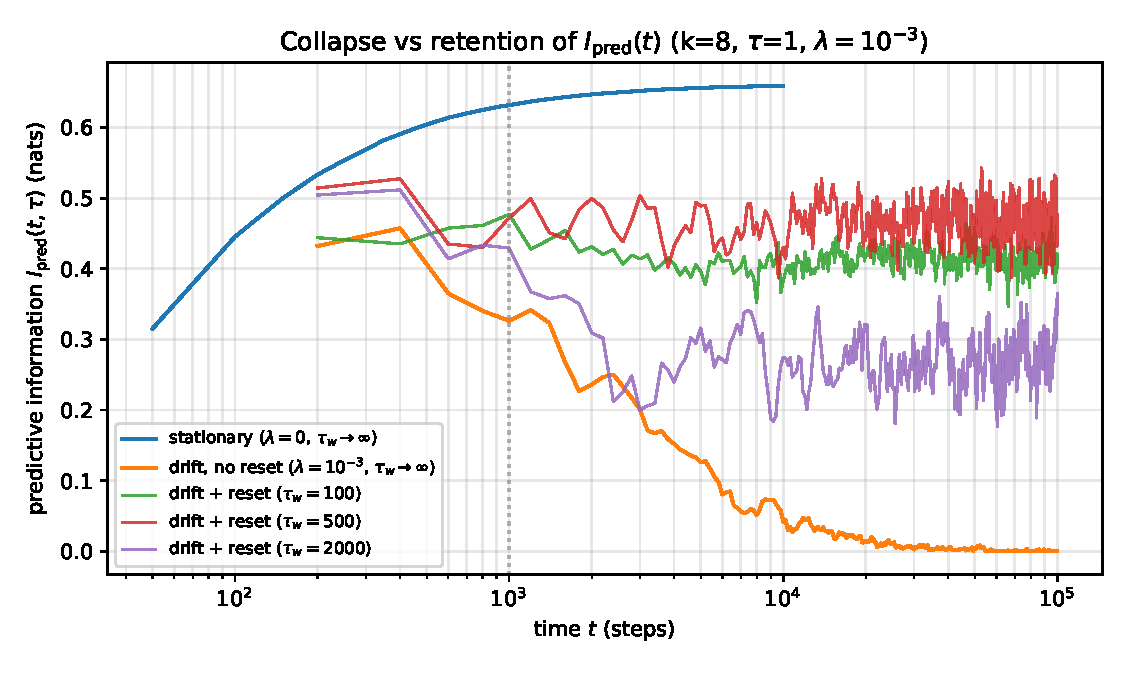
\includegraphics[width=0.85\linewidth]{figs/Fig1.pdf}\end{center}

 Диагностически ведущий числитель. В \textbf{стационарном} режиме (\(\lambda = 0\), \(\tau_w \to \infty\), \(T_{\text{sim}} = 10^4\)) \(I_{\text{pred}}\) \emph{удерживается} на \(\langle I_{\text{pred}}\rangle = 0{,}658 \pm 0{,}012\) нат --- оценка догоняет статику среды, \(\langle\nu^{\text{op}} \rangle = 0{,}006\). В режиме \textbf{дрейфа без сброса} (\(\lambda = 10^{-3}\), \(\tau_w \to \infty\), \(T_{\text{sim}} = 10^5\)) \(I_{\text{pred}}\) \emph{коллапсирует} до \(0{,}0007 \pm 0{,}0002\) нат --- падение в \(\approx 940\) раз относительно стационара (ratio \(0{,}0011\)): наблюдатель усреднил \(\hat P\) по \(\sim 100\) независимым прошлым режимам и почти не предсказывает текущий \(P(t)\). В режиме \textbf{дрейфа со сбросом} (\(\tau_w \in \{100, 500, 2000\}\), \(T_{\text{sim}} = 10^5\)) \(I_{\text{pred}}\) \emph{удерживается} на положительном уровне (\(0{,}41\), \(0{,}47\), \(0{,}27\) нат соответственно) --- забывание спасает прогноз. Это центральный результат: коллапс \(I_{\text{pred}}\) под накоплением памяти и дрейфом, снимаемый сбросом.



\emph{Рис. 2: оптимальное забывание --- \(\langle I_{\text{pred}}\rangle\) как функция \(\tau_w\)} 

\begin{center}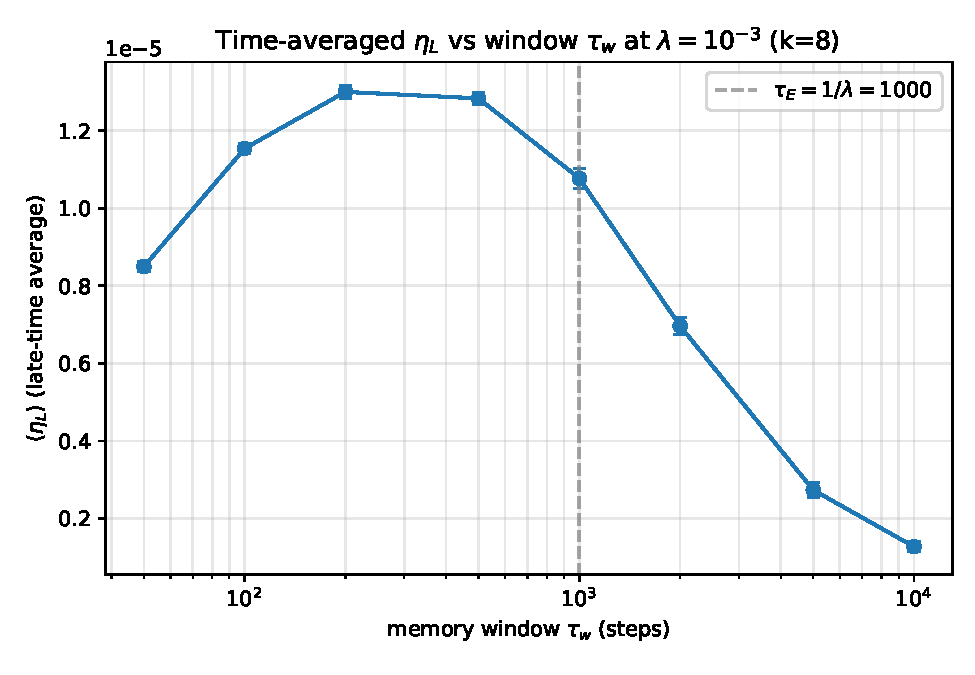
\includegraphics[width=0.85\linewidth]{figs/Fig2.pdf}\end{center}

 Куполообразная кривая (свип \(\tau_w \in \{50, \dots, 10^4\}\), \(\lambda = 10^{-3}\), \(T_{\text{sim}} = 5\cdot 10^4\)) с максимумом \(\langle I_{\text{pred}}\rangle^* = 0{,}467 \pm 0{,}006\) нат при \(\tau_w^* \approx 200\) шагов --- \emph{внутри} корреляционного интервала среды (\(\tau_w^* < \tau_E = 1000\)). Слишком короткое окно недооценивает \(\hat P\) (мало данных), слишком длинное усредняет несовместимые режимы; оптимум --- баланс. Это операциональная инстанциация (12) (\(\tau_{\text{reset}}^* < \tau_E\), \emph{забывать в темпе дрейфа}) с точностью до логарифмического множителя. (Вторичная ось \(\langle\eta_v\rangle\) структурно мала, \(\sim 3\cdot 10^{-3}\), и её собственный оптимум по \(\tau_w\) смещён к \(\approx 100\) --- это диагностика балласта, не качества прогноза.)



\emph{Рис. 3: ностальгия \(\nu^{\text{op}}(t)\) и \(\nu^{\text{Still}}(t)\)} 

\begin{center}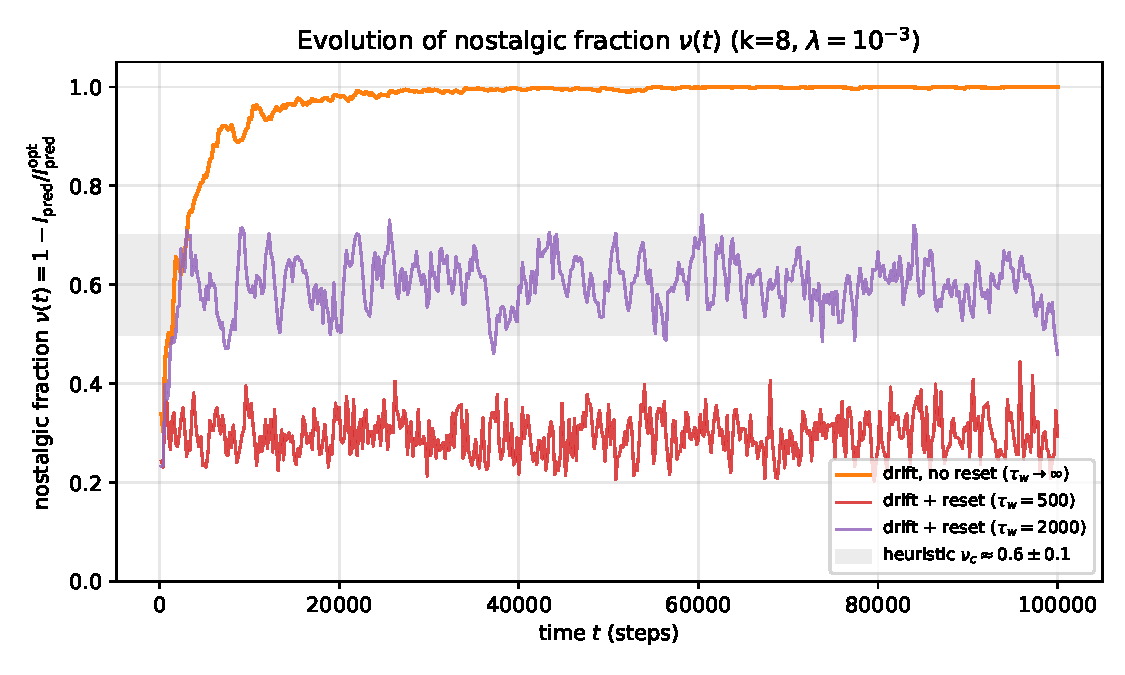
\includegraphics[width=0.85\linewidth]{figs/Fig3.pdf}\end{center}

 Операционально ведущая мера \(\nu^{\text{op}} = 1 - I_{\text{pred}}/I_{\text{opt}}\) (сплошные/штриховые кривые) \emph{различает режимы}: в дрейфе без сброса \(\nu^{\text{op}}(t) \to 0{,}999\) --- почти полная ностальгия (модель, накопленная по всем прошлым режимам, бесполезна для текущего); в режимах со сбросом \(\nu^{\text{op}}\) ограничена и зависит от \(\tau_w\) (\(0{,}38\) при \(\tau_w = 100\); \(0{,}30\) при \(\tau_w = 500\); \(0{,}60\) при \(\tau_w = 2000\)) --- минимум на оптимальном окне. Структурный балласт \(\nu^{\text{Still}} = 1 - \eta_v\) во \emph{всех} режимах с растущей памятью \(\approx 0{,}997\)--\(1{,}000\) --- почти вся удерживаемая память есть балласт; он \textbf{не различает} режимы (это структурное свойство накапливающего память обучателя, а не признак коллапса), и потому различающей шкалой выступает именно \(\nu^{\text{op}}\). Валидированные предельные случаи: при идеальном обучении \(I_{\text{pred}} \to I_{\text{opt}}\) (стационар, \(\nu^{\text{op}} \to 0\)); пол ёмкости и внутренний оптимум по \(\tau_w\) содержательны именно на шкале \(\nu^{\text{op}}\).



Проверки на всех \(1{,}36 \cdot 10^5\) выборенных точках: \(\eta_v \in [0, 0{,}006]\) (ограниченность обеспечена конечно-выборочным усечением § 3.1, а не наблюдена). Содержательная проверка пола (8a) идёт на шкале недобора \(\nu^{\text{op}} = \nu^{\text{theor}}\) (доступен оракул) --- см. § 6.3; балластное \(\nu^{\text{Still}} \to 1\) тривиально (§ 4.4) и полом не является. Полные параметры трёх режимов и сетки \(\tau_w\), псевдокод симуляции (взаимная информация в марковской модели считается точно по переходной структуре, без выборочного оценщика; выборочные оценщики Treves and Panzeri 1995, Kraskov et al.~2004 --- для данных реальных систем, § 3), обсуждение куполообразной зависимости как bias-variance компромисса, расхождение \(C_v^{\text{static}}/C_v^{\text{predictive}}\) как диагностического сигнала ностальгии --- Supplementary § S6.



\subsection{OU-симуляция: непрерывный дрейф логитов}\label{ou-ux441ux438ux43cux443ux43bux44fux446ux438ux44f-ux43dux435ux43fux440ux435ux440ux44bux432ux43dux44bux439-ux434ux440ux435ux439ux444-ux43bux43eux433ux438ux442ux43eux432}



OU-симуляция при \(\sigma = 0{,}1\), \(\lambda = 10^{-3}\) (\(\sigma^2/\lambda = 10\), стационарная дисперсия \(\sigma^2/(2\lambda) = 5\), \(k = 8\), \(K = k(k-1) = 56\), \(T_{\text{sim}} = 2 \cdot 10^4\) шагов, 50 реализаций) --- численная иллюстрация Леммы 2 в каноническом классе медленного дрейфа § 5.2 и центрального тезиса § 5.2 о том, что \textbf{дизайн памяти решает}. На \emph{одной} OU-траектории логитов (непрерывный дрейф без обнуления апостериора, в отличие от PSP-суррогата § 6.1) сравниваются два обучателя:



\begin{itemize}

\tightlist

\item

  \textbf{Роббинс--Монро} --- затухающий шаг \(\eta_t = c_0/\sqrt t\), \(c_0 = 3\) (асимптотически Bayes-оптимален для \emph{стационарных} регулярных моделей; Clarke and Barron 1990);

\item

  \textbf{постоянный шаг} \(s\) (рабочая точка \(s = 0{,}3\), валидированно близкая к оптимуму при \(\sigma = 0{,}1\)).

\end{itemize}



Условие slow-driving \(\lambda \tau_{\text{relax}} \ll 1\) выполнено с большим запасом; OU-concentration (\(\sigma^2/\lambda \ll 1\)) не выполняется, поэтому гипотеза Supplementary § S8.1 здесь не тестируется. Общий \(I_{\text{opt}} = 0{,}757 \pm 0{,}005\) нат (потолок предсказуемости), \(I_{\text{mem}} = 268{,}7\) нат, \(N_{\text{obs}} = t\). Значения --- поздневременные средние (последние 50\%, \(\pm\) SEM по 50 реализациям).



\emph{Почему ведущая мера --- \(\nu^{\text{op}}\), а не \(\eta_v\).} Ёмкость памяти здесь фиксирована (\(K\) параметров), и фигуры отчитываются по недобору прогноза \(\nu^{\text{op}}\) (нормировка на оптимум среды \(I_{\text{opt}}\)), а не по \(\eta_v = I_{\text{pred}}/I_{\text{mem}}\). Это намеренно: \(\nu^{\text{op}}\) изолирует нетривиальный пол ностальгии (грань B, § 1) от структурного роста знаменателя \(I_{\text{mem}}\) (грань A), который увёл бы \(\eta_v \to 0\) независимо от качества слежения. Наблюдаемое замерзание против отслеживания --- эффект \emph{схемы обновления памяти}, а не арифметики знаменателя.



\emph{Рис. 4: ностальгия \(\nu^{\text{op}}(t)\) обоих обучателей} 

\begin{center}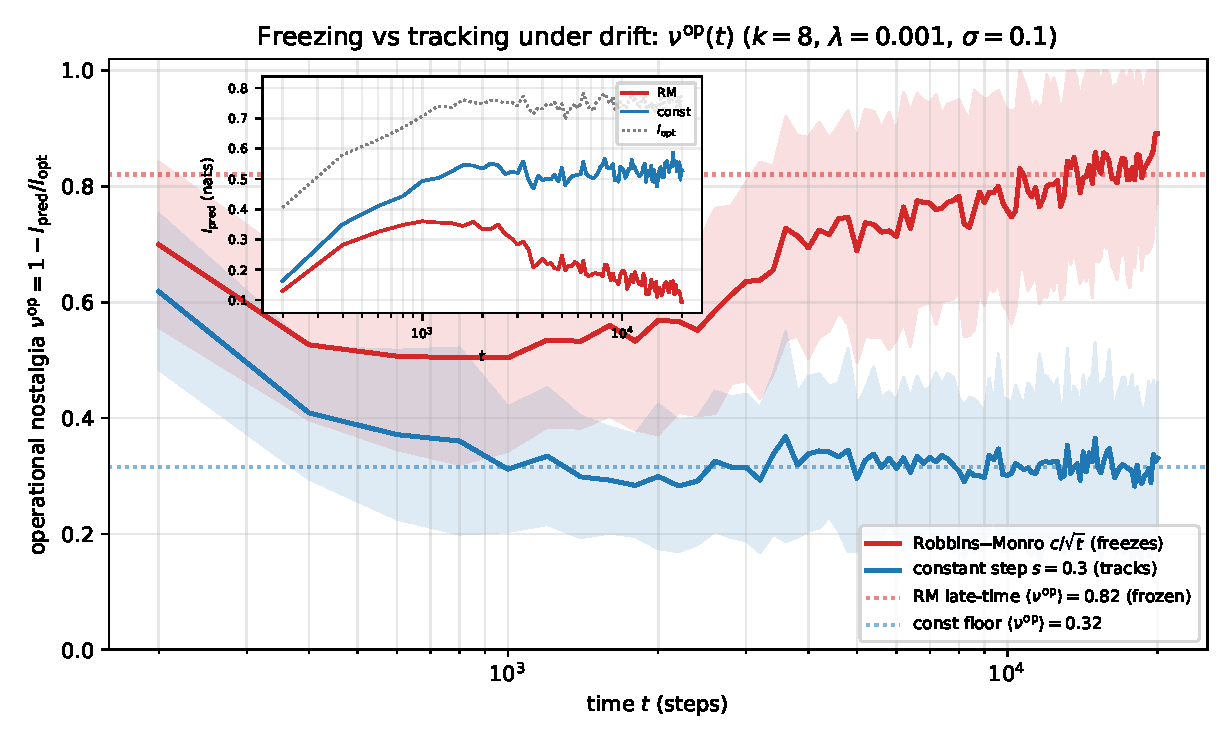
\includegraphics[width=0.85\linewidth]{figs/Fig4.pdf}\end{center}

 Несущая фигура. Обучатель \textbf{Роббинса--Монро замерзает} под дрейфом: его шаг затухает быстрее, чем дрейфует среда, оценка перестаёт отслеживать движущийся \(\theta_v(t)\), и \(\nu^{\text{op}}(t)\) монотонно \emph{растёт} \(0{,}567 \to 0{,}747 \to 0{,}892\) (в \(t = 2200, 10200, 20000\)), к поздневременному \(\langle\nu^{\text{op}}\rangle = 0{,}821 \pm 0{,}005\) (\(I_{\text{pred}} = 0{,}146\) нат, \(\theta_v\)-ошибка \(15{,}4\)). Обучатель с \textbf{постоянным шагом отслеживает} дрейф: \(\nu^{\text{op}}(t)\) держится на \emph{полу} \(\approx 0{,}33\) (\(0{,}283 \to 0{,}305 \to 0{,}331\)), поздневременное \(\langle\nu^{\text{op}}\rangle = 0{,}316 \pm 0{,}003\) (\(I_{\text{pred}} = 0{,}529\) нат --- в \(3{,}6\) раза выше RM). Вставка показывает \(I_{\text{pred}}(t)\) обоих против \(I_{\text{opt}}\): RM коллапсирует, постоянный шаг держится ниже оптимума на фиксированную цену запаздывания. Это прямая иллюстрация § 5.2: замерзание против отслеживания определяется \emph{схемой обновления памяти}, а не только средой.



\emph{Рис. 5: оптимальный размер шага} 

\begin{center}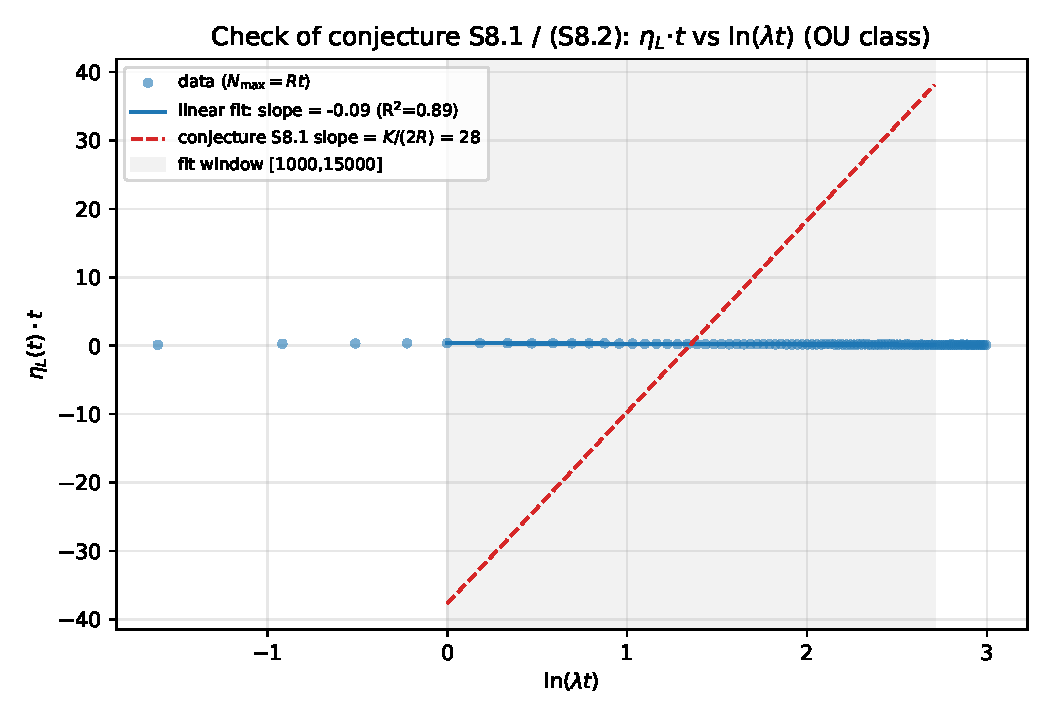
\includegraphics[width=0.85\linewidth]{figs/Fig5.pdf}\end{center}

 Свип размера постоянного шага при \(\sigma = 0{,}1\) показывает немонотонный пол \(\langle\nu^{\text{op}}\rangle(s)\) с \textbf{внутренним оптимумом} \(s^\star \approx 0{,}6\), \(\langle\nu^{\text{op}}\rangle = 0{,}290 \pm 0{,}004\): малый шаг (\(s = 0{,}02\): \(\nu^{\text{op}} = 0{,}861\)) даёт запаздывание (под-отслеживание), большой (\(s = 1{,}0\): \(\nu^{\text{op}} = 0{,}339\)) --- шум переобучения; между ними оптимум. Все точки свипа уверенно бьют замёрзший Роббинс--Монро (\(\langle\nu^{\text{op}}\rangle = 0{,}820\), пунктир). Свип по силе дрейфа \(\sigma\) подтверждает разводку: RM держится плоско-высоко (замёрз) на \(\nu^{\text{op}} \approx 0{,}82\)--\(0{,}86\) во всём диапазоне \(\sigma \in [0{,}03, 0{,}4]\), тогда как постоянный шаг \emph{отзывчив} к дрейфу (\(\nu^{\text{op}}\) от \(0{,}67\) при \(\sigma = 0{,}03\) до \(0{,}32\) при \(\sigma = 0{,}1\)). Содержательно: оптимальный обучатель забывает в темпе дрейфа; это связывает результат с continual learning --- замерзание RM есть тот же механизм, что катастрофическая потеря пластичности под distribution shift (§ 8.4).



Проверки на всех \(5 \cdot 10^4\) выборенных точках обоих обучателей: \(\eta_v \in [0, 0{,}008]\) (\(I_{\text{pred}} \le I_{\text{mem}}\) обеспечено усечением § 3.1); \textbf{содержательная} проверка --- недобор \(\nu^{\text{op}} \in [0{,}010, 1{,}000] \subset [0,1]\) с нулём случаев \(I_{\text{pred}} > I_{\text{opt}}\) (числитель \(\nu^{\text{op}}\) \emph{не} усекается). Балластная мера \(\nu^{\text{Still}} = 1 - \eta_v \approx 1\) для обоих обучателей (память фиксированного размера \(|M| = K\), но \(I_{\text{mem}} \gg I_{\text{pred}}\)): структурно \(\approx 1\), не различает замерзание от отслеживания --- различает именно \(\nu^{\text{op}}\), поэтому она и несущая.



Полные параметры обоих обучателей, асимптотическая Bayes-оптимальность Роббинса--Монро для \emph{стационарного} случая и её срыв под дрейфом, свипы \(\sigma\) и размера шага, обоснование рабочей точки \(s = 0{,}3\) --- Supplementary § S6. Полные параметры воспроизводимости (зерно \texttt{SEED\ =\ 20260524}, директории, версии библиотек) --- Supplementary § S4.



\subsection{Выводы симуляций}\label{ux432ux44bux432ux43eux434ux44b-ux441ux438ux43cux443ux43bux44fux446ux438ux439}



Две симуляции --- PSP (§ 6.1) и OU (§ 6.2) --- выполняют \textbf{пять конкретных функций} по отношению к формальной теории §§ 4--5. Они \textbf{не} претендуют на эмпирическую валидацию на реальных биологических системах (это задача pre-registered протоколов § 8.6) и \textbf{не} тестируют гипотезу Supplementary § S8.1 об адиабатической асимптотике \(L_{\text{excess}}\) (для неё нужно условие OU-concentration \(\sigma^2/\lambda \ll 1\), не выполненное ни в PSP, ни в OU § 6.2; соответствующий параметрический скан --- Supplementary § S8.3).



\textbf{(1) Коллапс \(I_{\text{pred}}\), спасаемый забыванием (три режима § 5.1).} PSP воспроизводит все три режима на диагностически ведущем числителе \(I_{\text{pred}}\): \emph{удержание} в стационаре (\(0{,}658\) нат), \emph{коллапс} при дрейфе без сброса (\(0{,}0007\) нат --- падение в \(\approx 940\) раз) и \emph{удержание при сбросе} (\(0{,}27\)--\(0{,}47\) нат). OU воспроизводит ту же развилку на непрерывном дрейфе через \emph{дизайн обучателя}: Роббинс--Монро коллапсирует (замерзает, \(I_{\text{pred}} = 0{,}146\) нат), постоянный шаг удерживает (\(0{,}529\) нат). Центральный результат --- коллапс \(I_{\text{pred}}\) под накоплением памяти и дрейфом, снимаемый забыванием/сбросом --- \emph{подтверждён} в обеих параметризациях.



\textbf{(2) Дизайн памяти решает (§ 5.2).} OU-симуляция прямо инстанциирует тезис: обучатель Роббинса--Монро (затухающий шаг, Bayes-оптимальный для стационара) под дрейфом \textbf{замерзает} --- \(\nu^{\text{op}}\) растёт \(0{,}567 \to 0{,}892\); постоянный шаг \textbf{отслеживает} к полу \(\nu^{\text{op}} \approx 0{,}32\). Свип по \(\sigma\) подтверждает: RM плоско-высок (\(\nu^{\text{op}} \approx 0{,}82\)--\(0{,}86\), нечувствителен к дрейфу --- замёрз), постоянный шаг отзывчив. Существует \textbf{оптимальный шаг} \(s^\star \approx 0{,}6\) (\(\nu^{\text{op}} = 0{,}290\)), бьющий замёрзший RM (\(0{,}820\)). Смысл --- забывать в темпе дрейфа: ни медленнее (замерзание), ни быстрее (шумовое переобучение).



\textbf{(3) Лемма 2: пол ностальгии выполнен.} PSP с дрейфом без сброса даёт \(\nu^{\text{op}}_\infty \to 0{,}999\) на operationally-ведущей шкале недобора прогноза --- это и есть прямая проверка пола (8a): при почти нулевом темпе обновления \(\dot M_{\text{refresh}} \to 0\) фракция \(c = \dot M_{\text{refresh}}\,\tau_E/|M_{\le t}| \to 0\), и \(\nu^{\text{op}} \ge 1 - c \to 1\) (наблюдено \(0{,}999\)). Структурный балласт \(\nu^{\text{Still}} \to 1{,}000\) на своей шкале тривиален и режим \emph{не} проверяет (§ 4.4). В OU постоянный шаг удерживает \(\nu^{\text{op}}\) ниже единицы именно потому, что обновляет память в темпе дрейфа (фракция \(c\) велика) --- согласовано с тем, что пол Леммы \(1-c\) тем ниже, чем выше темп refresh относительно \(\tau_E\). Количественная проверка границы \(1-c\) как \emph{точечного} предсказания на конкретной системе с контролируемым \(\tau_E\) откладывается на pre-registered протокол на E. coli (§ 8.6).



\textbf{(4) Существование \(\nu_c\) и оптимального забывания (§§ 5.3, (12)).} Куполообразная кривая \(\langle I_{\text{pred}} \rangle(\tau_w)\) (Рис. 2) с максимумом \(\langle I_{\text{pred}}\rangle^* = 0{,}467\) нат при \(\tau_w^* \approx 200 < \tau_E = 1000\) --- операциональная инстанциация (12) (\(\tau_{\text{reset}}^* < \tau_E\)) с точностью до логарифмического множителя; существование оптимума как функции структурных параметров (\(\tau_E\), \(\dot M_{\text{refresh}}\), \(|M_{\le t}|\)) --- измеримый эффект на синтетическом benchmark, не постулат. Непрерывный аналог --- оптимальный шаг \(s^\star \approx 0{,}6\) (Рис. 5). Это даёт \textbf{операциональную зацепку} для pre-registered предсказания П.1 (§ 8.6): расхождение \(C_v^{\text{static}}/C_v^{\text{predictive}}\) как диагностического сигнала режимного порога \(\nu_c\) на шкале недобора прогноза (open problem количественной формулы --- § 8.5).



\textbf{(5) Мост к continual learning (§ 8.4).} Замерзание Роббинса--Монро под дрейфом структурно эквивалентно катастрофической потере пластичности online-обучателя под distribution shift; постоянный шаг --- режиму непрерывной адаптации. Важная оговорка: наивная ML-форма предсказания (монотонный рост \(\nu^{\text{op}}\) с силой дрейфа для \emph{любого} обучателя) опровергается тем, что постоянный шаг \emph{не} следует ей --- устойчивость к дрейфу есть свойство дизайна памяти, а не неизбежность; несущий фальсификатор переноса Леммы 2 остаётся биологическим (E. coli, § 8.6).



\textbf{Что симуляции провалидированы.} На всех выборенных точках: \(\eta_v \in [0,1]\) (ограниченность обеспечена конечно-выборочным усечением \(I_{\text{pred}} \gets \min(I_{\text{pred}}, I_{\text{mem}})\) § 3.1 --- guard оценщика, не подтверждение границы); \textbf{содержательная} проверка --- \(\nu^{\text{op}} \in [0,1]\) с нулём случаев \(I_{\text{pred}} > I_{\text{opt}}\) на \(1{,}36 \cdot 10^5\) точках PSP и \(5 \cdot 10^4\) точках OU (числитель \(\nu^{\text{op}}\) не усекается). Предельные случаи воспроизведены: идеальное обучение \(I_{\text{pred}} \to I_{\text{opt}}\) (\(\nu^{\text{op}} \to 0\)) в стационаре; полный коллапс (\(\nu^{\text{op}} \to 1\)) при дрейфе без обновления; внутренний оптимум забывания. Балластный пол Леммы 2 выполнен (п. 3).



\textbf{Что симуляции \emph{не} делают.} (а) Не валидируют теорию на реальных биологических системах --- это задача § 8.6 П.2 (E. coli chemotaxis). (б) Не доказывают гипотезу Supplementary § S8.1 об асимптотике \((K/2)\ln(\lambda t)\) для \(L_{\text{excess}}\) --- нужен адиабатический OU-режим \(\sigma^2/\lambda \ll 1\), тестируемый отдельно в Supplementary § S8.3 (статус: открытая гипотеза, не теорема). (в) Не закрывают перенос Леммы 2 на не-OU классы (multi-scale drift, fractional OU) --- Замечание 4 § S5.1 ограничивает строгое доказательство OU-классом.



\emph{Оговорка о структуре \(\eta_v\).} \(\eta_v \sim 10^{-3}\) структурно мала во всех режимах с растущей памятью (грань A, § 1) --- это не сигнал качества («высока»/«катастрофически низка»), а свойство накопления; режимы различает \(\nu^{\text{op}}\), а \(\nu^{\text{Still}}\) несёт термодинамический бонд.



Резюме: симуляции подтверждают качественную структуру теории и дают операциональную зацепку для pre-registered предсказаний (П.1, П.2 § 8.6), оставаясь в области применимости через явное соблюдение \((*)\) и slow-driving.



\section{Связь с active inference и обучением без учителя}\label{ux441ux432ux44fux437ux44c-ux441-active-inference-ux438-ux43eux431ux443ux447ux435ux43dux438ux435ux43c-ux431ux435ux437-ux443ux447ux438ux442ux435ux43bux44f}



Связь между \(\eta_v\) и принципом свободной энергии Фристона (Friston 2010; Friston et al.~2017a) сформулирована в (Andriishin 2026, § 4.4): требование self-payment превращает FEP в дискриминационный критерий, а \(\eta_v\) операционально закрывает зазор между общим формализмом и требованием принадлежности энергии моделирующему контуру. В нестационарном режиме демаркация Pearl/Friston-blanket (Bruineberg et al.~2018; Bruineberg et al.~2022) сохраняется: соответствие \(\eta_v\) и EFE имеет смысл только для систем, проходящих тест самооплаты (\(S=1\), § 2.7); self-payment здесь --- \emph{альтернативная} онтология, а не конституирование Friston-blanket (ср. Andriishin 2026, § 4.4: вопрос сдвигается с «существует ли Friston-blanket» на «оплачивается ли удержание модели»). Для систем без самооплаты (\(S=0\)) соответствия нет.



В нестационарном режиме \(\eta_v(t)\) структурно соответствует эпистемической компоненте expected free energy \(G[\pi]\) (Friston et al.~2017a; Parr et al.~2022) в slow-driving пределе. \textbf{Это соответствие фиксируется как \emph{heuristic correspondence} (Supplementary § S7.1), не как доказанное неравенство}; гипотеза об эквивалентном неравенстве (Supplementary § S7.2) --- открытая задача. Категориальная оговорка: \(I_q(s'; o' \mid \pi)\) эпистемическая ценность AIF и \(I(X_t; X_{t+\tau} \mid \hat P(t))\) настоящей работы --- разные объекты MI (политикоконтекстная против наблюдательной); мост через достаточность \(\hat P(t)\) даёт нижнюю границу на эпистемическую ценность (эквивалентно --- верхнюю границу на \(I_{\text{pred}}\), Supplementary § S7.3), не равенство. Соответствие \emph{частичное в эпистемической компоненте}, не эквивалентность; прагматическая компонента через преференцию \(C\) остаётся вне термодинамической шкалы. \emph{Гипотетический} алгоритм active inference с расширенной целевой функцией, включающей \(\dot E_{\text{store}}\) в прагматическую часть преференций, балансировал бы снижение ностальгии и эксплуатацию модели с оптимумом (12); существующие AIF-имплементации (Friston et al.~2017a; Parr et al.~2022; Friston et al.~2021) оптимизируют \(G[\pi]\), не \(\eta_v(t)\). Связь с intrinsic motivation (Schmidhuber 1991; Friston et al.~2017b) и meta-learning (Finn et al.~2017): в нестационарной среде exploration \emph{информационно} необходим для \(\eta_v > 0\) (без обновления памяти \(I_{\text{pred}} \to 0\); термодинамика входит через цену удержания, не как источник самой необходимости).



\emph{Метрика информационного омоложения.} Отношение темпов обновления и роста памяти



\begin{equation}\rho(t) = \frac{\dot{M}_{\text{refresh}}(t)}{\dot{M}_{\text{grow}}(t)} \tag{13}\end{equation}



--- диагностика, независимая от прямого измерения \(\nu(t)\): \(\rho \gg 1\) --- обновление обгоняет рост, ностальгия низкая; \(\rho \ll 1\) --- архивный слой ностальгизируется. Эмпирическая калибровка \(\rho_c\) --- отдельное исследование.



Полное формальное соответствие \(\eta_v\) и EFE с конверсией единиц через \(\beta_v = 1/(k_B T)\), heuristic correspondence для приращения \(\Delta G^{\text{epist}}\) против \(\Delta I_{\text{pred}}\), гипотеза об эквивалентном неравенстве, категориальная оговорка \(I_q(s'; o') \ne I(X_t; X_{t+\tau})\), контекст sophisticated inference (Friston et al.~2021), парирование Andrews (2021) / Williams (2020) через перекрёстную ссылку на (Andriishin 2026, § S4.4a), разбор метрики информационного омоложения \(\rho(t)\) (полюса refresh/grow и её бактериальная инстанциация) --- Supplementary § S7.



\section{Обсуждение, открытые вопросы и заключение}\label{ux43eux431ux441ux443ux436ux434ux435ux43dux438ux435-ux43eux442ux43aux440ux44bux442ux44bux435-ux432ux43eux43fux440ux43eux441ux44b-ux438-ux437ux430ux43aux43bux44eux447ux435ux43dux438ux435}



\subsection{Итоги}\label{ux438ux442ux43eux433ux438}



Работа методологически расширяет (Andriishin 2026) на нестационарный режим: три структурных результата, методологический инструментарий, одна открытая количественная гипотеза.



\textbf{Три структурных результата.}



\begin{enumerate}

\def\labelenumi{\arabic{enumi}.}

\item

  \emph{Цена растущей памяти (Лемма 1 и термодинамический пол).} Предсказательная эффективность \(\eta_v(t)\) измеряется на \emph{растущем} знаменателе --- полной удерживаемой памяти, которая копится по мере обучения (§ 2.1, § 5.1). Термодинамическая цена этого удержания вынесена в отдельную, кумулятивную форму бонда Still: за всю историю система диссипирует не меньше, чем «стоит» удержанный непредсказательный балласт (§ 2.2). Лемма 1 даёт минимальную мощность, необходимую, чтобы удержать один бит против термодинамической эрозии (§ 2.3).

\item

  \emph{Ностальгия на растущей памяти (Лемма 2).} Предсказательная информация обобщена на полную --- актуальную плюс архивную --- память (§ 3), а сама ностальгия разведена на две линии: операционально ведущий \emph{недобор прогноза} (в теоретической и в измеримой версиях) и вторичный структурно-термодинамический \emph{балласт}, несущий бонд Still (§ 4.1). Лемма 2 даёт \emph{условный} пол: при медленном гауссовском дрейфе (OU-класс § 5.2) и конечном темпе обновления недобор прогноза асимптотически не падает ниже вычислимой границы \(1 - \kappa c\) (\(\kappa = 1 + o(1)\) эмпирически, § 4.4), а эффективность \(\eta_v(t)\) проходит три режима (§ 5.1).

\item

  \emph{Порог и оптимальный сброс.} Выделяется режимный порог \(\nu_c\), разделяющий адаптивную память и ностальгический коллапс (§ 5.3), и оптимальный интервал периодического сброса памяти \(\tau_{\text{reset}}^*\), созвучный шкале эпигенетического перепрограммирования (§ 5.3).

\end{enumerate}



\emph{Методологический инструментарий:} различение теоретического и измеримого недобора прогноза (§ 4.1); статическая против предсказательной операционализация ёмкости самомодели как диагностика ностальгии (§ 4.3); дисциплина протокола против ad hoc спасений (§ 5.2, Supplementary § S5.2); и два pre-registered протокола (§ 8.6).



\textbf{Количественная гипотеза вынесена в Supplementary § S8.} Отдельная догадка об адиабатической асимптотике накопленного предсказательного проигрыша --- \emph{неподтверждённая вторичная надстройка}, а не результат работы: численный скан поддерживает её функциональную форму, но не отличает медленной сходимости к пределу от плато ниже него, и потому мы не заявляем её как достижимый закон. Несущее ядро работы от неё не зависит; техническая сверка коэффициентов --- § S8.3.



\emph{Сильнейшее возражение и ответ на него.} Назовём самое острое возражение прямо: вынесенная в supplementary адиабатическая асимптотика не прошла независимых численных проверок (§ 6, § 8.5) и остаётся неподтверждённой гипотезой, а не результатом. Ответ: несущее ядро работы от неё \emph{не зависит} --- Леммы 1 и 2, вычислимая граница недобора прогноза, разделение балласта и недобора, критерий self-payment и методологический протокол доказаны или сформулированы независимо от этой асимптотики. Её опровержение не затрагивает ни одного ядрового утверждения.



Численные иллюстрации (§ 6) демонстрируют Лемму 2 и три режима \(\eta_v(t)\); эффективность \(\eta_v(t)\) соответствует эпистемической компоненте ожидаемой свободной энергии активного вывода (§ 7), где вводится и метрика информационного омоложения \(\rho(t)\).



\textbf{Структурные результаты и контекст-зависимые спецификации.} \emph{Структурные результаты} (общие утверждения, независимые от выбора параметрического класса): self-payment на нестационарном режиме (§ 2.7); стационарный результат статьи \#1 как частный случай; \(\eta_v(t) \in [0, 1]\) по DPI для концептуального числителя (§ 2.1); кумулятивный бонд Still ((2-кум), § 2.2) и Лемма 1; Лемма 2; существование \(\nu_c^{\text{theor}}\) на шкале недобора прогноза (с рабочим допущением о стабильности под сменой нормировки, § 4.1); разделение ностальгии-балласта \(\nu\) и недобора прогноза \(\nu^{\text{theor}}\)/\(\nu^{\text{op}}\); протокол § 5.2 / Supplementary § S5.2. \emph{Контекст-зависимые спецификации} (зависят от конкретного параметрического класса или операционального выбора): класс дрейфа (OU/PSP --- кусочно-стационарный); численная оценка \(\nu_c^{\text{op}}\); выбор окна \(\tau\); операционализации ёмкости самомодели \(C_v\) (статья \#1); открытая количественная гипотеза Supplementary § S8.



\subsection{Что НЕ делается в этой работе}\label{ux447ux442ux43e-ux43dux435-ux434ux435ux43bux430ux435ux442ux441ux44f-ux432-ux44dux442ux43eux439-ux440ux430ux431ux43eux442ux435}



Работа ограничивается теорией. За пределами --- (i) эмпирическая калибровка \(\eta_v(t), \nu(t), \rho(t)\) на конкретных биосферах, городах, LLM (требует операционализации \(E_{\text{store}}, E_{\text{grow}}\) для каждого класса); (ii) полная теория когнитивных систем как \(\eta_v\)-проблема (психологическая память, забывание, бытовая ностальгия как феноменальные состояния субъекта --- категориально отличный референт от информационной ностальгии настоящей работы); (iii) философские следствия различения актуального и архивного слоёв памяти (семантическая против эпизодической памяти, роль забывания в идентичности).



\subsection{LLM-corp как межпредметная иллюстрация (пограничный случай)}\label{llm-corp-ux43aux430ux43a-ux43cux435ux436ux43fux440ux435ux434ux43cux435ux442ux43dux430ux44f-ux438ux43bux43bux44eux441ux442ux440ux430ux446ux438ux44f-ux43fux43eux433ux440ux430ux43dux438ux447ux43dux44bux439-ux441ux43bux443ux447ux430ux439}



Класс крупных языковых моделей, обученных на статичном корпусе и эксплуатируемых в дрейфующей среде, фигурирует как \emph{межпредметная иллюстрация} применимости формализма к не-биологическим системам, не как самостоятельное эмпирическое приложение (центральное предсказание работы --- chemotaxis \emph{E. coli}, § 8.6 П.2).



\emph{Граница и self-payment} (§ 2.7). В строгой LLM-as-agent без сохранения состояния контур самооплаты структурно незамкнут: \(\dot E_{\text{store}}\) оплачивается внешним дата-центром, и \(\eta_v\) не определён. По escalating boundaries paper \#1 (Andriishin 2026, § 3.4 + Supplementary § S3.4) \(\eta_v(t)\) определён лишь начиная с \(B_4\)-границы (корпорация-юр.лицо): актуальный слой \(M_t\) --- KV-cache плюс операционное состояние корпорации, архивный \(M_{\lt t}\) --- веса плюс корпоративный корпус, среда \(X_E\) --- статистика запросов, дрейфующая по словарю (Lazaridou et al.~2021; Dhingra et al.~2022). Это \emph{честное понижение в статусе}: формализм сам выводит незамкнутые конфигурации из области применимости, а не натягивается на них.



\emph{Двухслойное предсказание.} Для архивного слоя переобученной LLM без continual pre-training (\(\dot{M}_{\text{refresh}}^{\lt t} \approx 0\), \(c \approx 0\)) Лемма 2 даёт \(\liminf \nu_{\lt t}(t) \ge 1\) --- веса устаревают по мере дрейфа языка, что качественно есть монотонный рост perplexity на текстах после момента отсечки --- \textbf{известное наблюдение} (Lazaridou et al.~2021; Dhingra et al.~2022), не оригинальное предсказание. Для актуального слоя моделей с длинным контекстом \(c\) для \(M_t\)-слоя \(\gg 1\), и Лемма 2 \emph{на нём не применима} (режим скользящего окна, явное самоограничение через \((*)\)).



\emph{Каналы refresh и open question.} In-context learning обновляет лишь \(M_t\); continual pre-training и RAG с обновляемым индексом (Lewis et al.~2020; Borgeaud et al.~2022; Khandelwal et al.~2020; Izacard et al.~2023) --- refresh-канал для \(M_{\lt t}\) (сравнение perplexity с/без обновляемого RAG --- операциональное предсказание). Открытый вопрос: индуцирует ли \emph{неявная in-context-адаптация} (induction heads --- Olsson et al.~2022; ICL функциональных классов --- Garg et al.~2022; Bricken et al.~2023) неявное обновление архивного слоя; если нет --- \(\nu_{\lt t} \to 1\) остаётся для всех LLM с длинным контекстом без RAG.



\subsection{Связь с continual learning}\label{ux441ux432ux44fux437ux44c-ux441-continual-learning}



Catastrophic forgetting (McCloskey and Cohen 1989; Goodfellow et al.~2014; Kirkpatrick et al.~2017; Lopez-Paz and Ranzato 2017; Riemer et al.~2019; Parisi et al.~2019) имеет естественную интерпретацию в рамках теории; параллельный аппарат --- стохастическая термодинамика обучения (Goldt and Seifert 2017). Concept drift (Gama et al.~2014; Bifet and Gavaldà 2007) объединяется через мост (8): drift-обнаружители срабатывают при \(\nu(t) > \nu_c\). Catastrophic forgetting --- \emph{провал} удержания предсказательной памяти (перезапись без выделения \(E_{\text{grow}}\)), а не намеренное уменьшение \(\nu(t)\). Методы борьбы ложатся на баланс по-разному: progressive networks и replay buffers --- инвестирование в \(E_{\text{grow}}\) (рост носителя), тогда как EWC (Kirkpatrick et al.~2017) --- регуляризация, \emph{защищающая} предсказательные веса от перезаписи (снижение \(\nu\) без роста ёмкости).



Ностальгия и catastrophic forgetting --- два полюса баланса \(\dot{E}_{\text{store}}\) и \(\dot{E}_{\text{grow}}\): ностальгия --- \emph{избыток} непредсказательной памяти, forgetting --- \emph{дефицит} преждевременно стёртой. Оптимум --- (12). При \(\lambda \to 0\) ностальгия редуцируется в \emph{переобучение}.



\emph{Контраст с переименованием --- сравнение с ML-прецедентами.} На возражение «ностальгия --- переименование concept drift + forgetting + dynamic regret»: теория содержит конструкции, структурно близкие к известным ML-результатам, но операционально и шкалово от них отличные.



\emph{Протокол сработал на самих авторах.} Пункт протокола (§ 5.2), запрещающий post-hoc переопределение объекта измерения, --- реальное ограничение, а не ритуал: соблазн заменить операционально измеримую \(I_{\text{pred}}\) на counterfactual \(L_{\text{excess}}\) (под которым асимптотика держится), сохранив имя теории, запрещён протоколом --- \(L_{\text{excess}}\) вынесена в § S8 как вторичная метрика, асимптотика помечена как открытая гипотеза (детали --- § 8.1).



\textbf{(a) Лемма 2 против Besbes--Gur--Zeevi 2015 (динамический регрет).} (Besbes et al.~2015) (Theorem 2) дают для sliding-window learner regret \(R_T = O(V_T^{1/3} T^{2/3})\); параллелизм очевиден. Различие: это \emph{sample-level upper bound} на regret при \(V_T = o(T)\), тогда как Лемма 2 --- \emph{информационная} нижняя граница на недобор прогноза \(\nu^{\text{theor}}(t)\) (недостижимую долю предсказуемого будущего) в OU-классе § 5.2, с отдельным термодинамическим полом удержания этой фракции через кумулятивный бонд Still ((2-кум), (8)), то есть нижняя граница на меру, которой sample-level regret не отражает.



\textbf{(b) \(\tau_{\text{reset}}^*\) против оптимальной длины скользящего окна (Hazan and Seshadhri 2009; Karnin and Anava 2016).} Там \(\tau_{\text{reset}}\) --- \emph{алгоритмический} restart-параметр без термодинамической интерпретации; в (12) --- \emph{физический} интервал периодического стирания памяти, оптимизирующий \(\eta_v\) через компромисс \(\dot E_{\text{store}}\) против \(\dot E_{\text{grow}}\) (биологическая инстанциация --- время поколения эпигенетического перепрограммирования, § 4.4).



\textbf{(c) \(\nu_c\) против фазовых переходов в ML.} \(\nu_c \in (0,1)\) (11) \emph{не} эквивалентно grokking (Power et al.~2022) (reorganisation весов при фиксированной среде) или double descent (Belkin et al.~2019) (обобщение против ёмкости при фиксированной задаче): \(\nu_c\) --- переход в \emph{memory composition} при дрейфующей среде и фиксированной архитектуре; связь нетривиальна (§ 8.5).



\textbf{(d) Термодинамическая шкала \(k_B T \ln 2\) отсутствует в ML-литературе.} Ностальгия как энергетическая величина там не определяется; \(\dot{E}_{\text{store}}^{\text{nostalg}} \ge k_B T \ln 2 / \tau_{1/2}\) --- мост между информационной мерой \(\nu\) и физическим бюджетом, неподнимаемый внутри ML-формализмов (Still et al.~2012; Gama et al.~2014; Kirkpatrick et al.~2017). В биологическом камертоне, напротив, энергетика адаптации --- установленный факт: цена точности и темпа сенсорной адаптации количественно описана для хемотаксиса \emph{E. coli} (Lan et al.~2012; Mehta and Schwab 2012). Вклад настоящей работы здесь не в первом введении энергетики в хемотаксис, а в \emph{нестационарной нижней границе на накопление ностальгии} --- на поток удержания устаревающей фракции памяти во времени, не на однократную адаптацию.



\emph{Операциональная зацепка на \(c\) для ML.} Для SGD со скоростью \(\eta_t\) на \(N\) параметрах при частоте перестановки \(\rho_p\) (\(\tau_E = 1/\rho_p\)) темп обновления \(\dot M_{\text{refresh}} \approx \eta_t N\), \(|M_{\le t}| \approx N\), откуда \(c \approx \eta_t/\rho_p\) (order-of-magnitude; точное значение калибруется эмпирически). Быстрый дрейф (большой \(\rho_p\)) даёт малый \(c\) и высокую ностальгию \(\nu \to 1-c\); медленный --- большой \(c\), режим скользящего окна, где Лемма 2 неприменима. Оговорка о классическом Permuted MNIST (Goodfellow et al.~2014): там каждая перестановка дообучается до сходимости, то есть смена \emph{редкая} (малый \(\rho_p\), большой \(c\)); и его метрика --- падение accuracy на прошлых задачах, а не \(\nu^{\text{op}}\), отождествлять нельзя.



\emph{ML-форма предсказания.} Наивно: для обучаемого MLP без EWC/replay ностальгическая фракция растёт с \(\rho_p\), где \(\nu^{\text{op}}\) проксируется ablation-долей --- долей скрытых юнитов, зануление которых \emph{не} повышает current-task loss. Это лишь \emph{прокси} канонической \(\nu^{\text{op}} = 1 - I_{\text{pred}}/\hat E\) (§ 4.1), не тождество, и требует контроля выученности.



\emph{Воспроизводимый камертон и честный отрицательный результат} (\texttt{simulations/permuted\_mnist/}: \texttt{sklearn.load\_digits} \(8\times8\), MLP \(64\to32\to10\), online SGD). Наивная форма \textbf{не выживает}: наивный прокси \(\nu^{\text{op}} \approx 1 - \text{выученность}\) \textbf{конфаундит ностальгию с недоучённостью} --- при быстром дрейфе сеть механически не успевает выучить задачу (accuracy \(\to\) chance), и прокси растёт безотносительно ностальгии. После accuracy-gate и определения \emph{истинной} ностальгии (юнит бесполезен сейчас \textbf{и} был полезен на недавней прошлой перестановке) эффект \textbf{исчезает и обращается} (\(\nu^{\text{op}}_{\text{true}}\) анти-коррелирует с \(\rho_p\); Спирмен \(= -1{,}0\) на четырёх усреднённых по зёрнам точках --- содержателен лишь знак (per-run распределения соседних \(\rho_p\) перекрываются); полные числа и разброс --- в README камертона). Причина: SGD --- high-refresh обучатель, постоянно в режиме большого \(c\) (скользящее окно), поэтому малый MLP \textbf{не} инстанциирует закон \(c \to \nu\) чисто; ведущий драйвер здесь --- ре-специализация при долгом dwell.



Содержательно это \textbf{третий честный negative-тест} статьи --- после проверки PSP-границы (§ 6.1) и OU-класса для адиабатической асимптотики (§ 6.2). Методологический протокол § 5.2 (приоритет фальсифицируемости над подтверждением) сработал и здесь: без контроля выученности confound-driven «подтверждение» было бы сохранено как валидное; контроль удержал от этого. Несущий фальсификатор Леммы 2 остаётся \textbf{биологическим} --- бактериальный хемотаксис \emph{E. coli} (§ 8.6); наивная ML-форма опровергнута собственным камертоном и не подаётся как подтверждение.



\emph{Class-restriction и no-free-lunch.} Wolpert no-free-lunch (Wolpert 1996) даёт фундаментальное обоснование сужения класса (§ 5.2): универсальная теория нестационарной обучаемости без априорного ограничения класса невозможна; class slow-driving --- одно из достаточных сужений (NFL обосновывает, что \emph{некоторое} сужение необходимо, а не именно это), выбранное как каноническое и биологически мотивированное.



\subsection{Открытые проблемы}\label{ux43eux442ux43aux440ux44bux442ux44bux435-ux43fux440ux43eux431ux43bux435ux43cux44b}



\emph{Три связанные открытые проблемы.} (i) перенос пола \(\liminf\nu^{\text{theor}} \ge 1-c\) за пределы OU-класса; (ii) статус адиабатической асимптотики \((K/2)\ln(\lambda t)\); (iii) поведение при сверхлинейном росте памяти \(|M_{\le t}| \propto t^\alpha\). Открыт и связанный концептуальный вопрос: \emph{отслеживает} ли термодинамическая цена удержания (балласт \(\nu^{\text{Still}}\), несущий бонд) режимный коллапс (недобор прогноза \(\nu^{\text{op}} \to 1\)), или стоит от него отдельно --- то есть сущностна ли видимая юкстапозиция структурного балласта и режим-различающего недобора.



\emph{Гипотеза об адиабатической асимптотике (Supplementary § S8).} Гипотеза Supplementary § S8.1 об асимптотике кумулятивной excess-loss \(L_{\text{excess}}(t) \sim (K/2)\ln(\lambda t)\) в OU-классе при \(\sigma^2/\lambda \ll 1\) остаётся \emph{открытой и неподтверждённой}. Аналитическое значение \(K/2\) выводится как тождество предела \(\epsilon_{\text{track}} \to 0\), и численный скан Supplementary § S8.3 поддерживает функциональную форму (\(R^2 \ge 0{,}9995\) в фите \(A t + B\ln(\lambda t) + C\)), однако подгоночный \(B/(K/2)\) растёт монотонно (0,54→0,85 при \(\sigma^2/\lambda\) от \(10^{-1}\) до \(10^{-3}\)), не достигая единицы. Такое поведение согласуется скорее с тем, что предел структурно \emph{недостижим} (адиабатический логарифм реализуется лишь транзиентно, после чего \(L_{\text{excess}}\) выходит на плато), чем с недобором точек скана. Мы поэтому \emph{не} заявляем асимптотику как достижимый закон; тем более открыт её перенос на операционально измеримую \(\eta_v(t)\) (\(\dot\eta_v^{\text{excess}}\)).



\emph{Расширение Леммы 2 на быстро растущую память.} Текущая Лемма 2 опирается на ограниченность \(|M_{\le t}|\) через константу \(c\) из \((*)\). При \(|M_{\le t}| \propto t^\alpha\) (\(\alpha \ge 1\)) условие \(c \lt 1\) становится тривиально выполнимым, но качественная картина ностальгии меняется: при достаточно быстром росте ёмкости ностальгическая фракция может оставаться конечной долей. Формальное расширение Леммы 2 на этот режим --- открытая задача нестационарных байесовских моделей.



\emph{Связь с fluctuation theorems.} Теоремы Crooks (Crooks 1999) и Jarzynski (Jarzynski 1997); обобщение с feedback-контролем (Sagawa and Ueda 2010) даёт мост к декомпозиции (1) через измерительный канал. Применение к балансу \(E_{\text{store}}, E_{\text{grow}}, E_{\text{actual}}^{\text{curr}}\) может дать более тонкие неравенства, чем ландауэровская граница.



\emph{Операционализация \(E_{\text{store}}\) для культурной и биосферной памяти.} \(\tau_{1/2}\) количественно различен (эпигенетика, геном, синапсы); в культурных системах носитель неоднозначен (книга, цифровой архив, нейронная сеть) --- отдельное исследование.



\emph{Уточнение режимного порога \(\nu_c\).} Существование строгого перехода с универсальными критическими показателями и численная оценка для камертонных классов --- открытый вопрос. Сюда же --- \emph{стабильность \(\nu_c\) под сменой нормировки} (§ 4.1): строгая теорема о монотонности режимного порога под DPI-неравенством \(\nu^{\text{op}} \le \nu^{\text{theor}}\), обосновывающая переход от \(\nu_c^{\text{theor}}\) к \(\nu_c^{\text{op}}\) в pre-registered протоколе § 8.6 (П. 1).



\emph{Аналитическое замыкание per-bit-uniformity.} Допущение per-bit-uniformity Замечания 5 (аддитивность MI по независимо обновляемым битам с константой \(1+o(1)\), § 4.4) в настоящей работе проверено \emph{численно} (§ 6.2) и опирается на вырожденность межкоординатной связи \(\kappa \to 0\) при параметрах OU-скана § 6.2 (независимость логитов, Supplementary § S2.2/§ S2.7); общего аналитического доказательства оно не имеет. При ненулевой связи \(\kappa > 0\) константа аддитивности отклоняется от \(1\), и переход от бит-доли \(c\) к информационному отношению \(\nu^{\text{theor}} \ge 1 - c\) требует отдельной оценки. Явная граница на \(|1 - \text{const}|\) как функция \(\kappa\) (аналитическое замыкание за пределами вырожденного режима § 6.2) --- открытая задача.



\emph{Регулярность softmax-параметризации.} Полное доказательство переноса OU-декорреляции на нелинейную softmax-параметризацию матрицы переходов (Замечание 6 § 4.4) --- техническое расширение через Lipschitz-непрерывность по total variation на ограниченной с вероятностью \(1-\delta\) части траектории OU; даёт сходимость \(\nu(t) \to 1 - c\) в конкретной OU-параметризации § 6.2 / Supplementary § S6.3 за пределами иллюстративного \(\liminf\)-неравенства (8a).



\subsection{Эмпирические предсказания}\label{ux44dux43cux43fux438ux440ux438ux447ux435ux441ux43aux438ux435-ux43fux440ux435ux434ux441ux43aux430ux437ux430ux43dux438ux44f}



Теория формулирует два ядрово-эмпирических предсказания (П. 1, П. 2).



\emph{Предсказание 1: существование режимного порога \(\nu_c^{\text{op}} \in (0, 1)\).} В адаптивных нестационарных системах с конечным темпом обновления памяти должен существовать критический уровень ностальгии \(\nu_c^{\text{theor}} \in (0, 1)\) (§ 5.3); операционально диагностируется через эмпирический порог \(\nu_c^{\text{op}}\) по расхождению \(C_v^{\text{static}}/C_v^{\text{predictive}}\) при наблюдаемом дрейфе среды (§ 4.3): при \(C_v^{\text{static}}/C_v^{\text{predictive}} \to \infty\) система пересекла \(\nu_c^{\text{op}}\) (см. рабочее допущение § 4.1 о связи \(\nu_c^{\text{theor}}\) и \(\nu_c^{\text{op}}\)). Опровержение: отсутствие расхождения двух прокси в системах с заведомо нарушенной адаптацией (например, замороженные LLM-веса в дрейфующем потоке запросов; полностью метилированные бактерии без активной деметилазной коррекции).



\emph{Предсказание 2: замедление adaptation rate при блокировке refresh-петли метилирования рецепторов (E. coli chemotaxis; качественное замедление + }различающий* количественный пол).* Биологическим камертоном Леммы 2 в бактериальной системе выступает адаптационная петля хемотаксиса: метилтрансфераза CheR ковалентно метилирует методил-акцептирующие хемотаксис-рецепторы (MCPs: Tar, Tsr, Tap, Trg) на консервативных глутаматных остатках; метилэстераза CheB активно деметилирует их в фосфорилированном режиме, замыкая negative-feedback контур точной адаптации (Yi et al.~2000; Alon et al.~1999; Sourjik and Berg 2002; Endres and Wingreen 2006). Метилированные состояния рецепторов реализуют \(M_{\le t}\) Леммы 2 (внутреннее состояние, хранящее статистику фоновой концентрации лиганда); CheR/CheB-опосредованное переметилирование --- \(\dot M_{\text{refresh}}\). \textbf{Качественное замедление} adaptation rate и интеракция генотип×среда --- \emph{необходимое, но не различающее} следствие: та же интеракция вытекает из стандартной кинетики адаптации (Endres and Wingreen 2006; Lan et al.~2012), где фильтр с большей постоянной времени хуже отслеживает быстрее флуктуирующий вход. \textbf{Различающим} служит \emph{количественный} пол: в лаборатории \(I_{\text{opt}}\) \emph{известен} (экспериментатор задаёт OU-статистику среды через профиль концентрации), поэтому retreat «нужен оракул» (§ 4.1) снят, и Лемма 2 даёт проверяемый пол \(\nu^{\text{op}}(t) \gtrsim 1-c\) с независимо измеримой \(c = \dot M_{\text{refresh}}\,\tau_E/|M_{\le t}|\) (оборот метилирования \(\to \dot M_{\text{refresh}}\); наложенное \(\tau_E\); \(|M_{\le t}| \sim\) число метил-сайтов \(\times\) копийность рецептора). Стандартные модели дают \emph{знак} замедления, но не \emph{значение} пола --- именно оно тестирует рамку ностальгии.



\emph{Протокол.} Подавление refresh-петли реализуется через \textbf{гипоморфный мутант CheR с пониженной активностью} (\(cheR^{\downarrow}\)) или контролируемое снижение экспрессии \emph{cheR} из титруемого (IPTG-индуцируемого) промотора (Alon et al.~1999, Fig. 2) --- это сохраняет точную адаптацию как функцию (в отличие от нокаута \(\Delta cheB\), дающего немедленный фенотип постоянного кувыркания через гипер-фосфорилирование CheY, не связанный с постепенным накоплением ностальгии Леммы 2). Среда --- \textbf{стохастически дрейфующий хемотактический градиент}: концентрация аспартата / α-methyl-DL-aspartate (MeAsp) для рецептора Tar (или серина для Tsr) модулируется \emph{шумовым процессом орнштейн-уленбековского типа} (экспоненциальная автокорреляция с временем \(\tau_E\)) в проточной микрофлюидной камере с известным профилем --- это ставит среду в тот же OU-класс медленного дрейфа, для которого доказана Лемма 2 (детерминированная периодическая смена НЕ годится: её автокорреляция не затухает экспоненциально, и pre-registered тест принадлежности класса п. 2 её отвергнет); константная концентрация --- контрольная среда. Характерное время дрейфа среды \(\tau_E = 5\)-- \(15\) минут (в пределах минутной шкалы метиляционного refresh --- Sourjik and Berg 2002; Endres and Wingreen 2006); горизонт эксперимента --- \(\ge 10\) поколений (типичное время поколения \emph{E. coli} в M9-минимальной среде 40--60 мин), что при \(\tau_E = 5\)--\(15\) мин даёт \(\gtrsim 30\) циклов дрейфа на горизонте --- с запасом над требуемыми 5--10.



\emph{Первичный показатель.} Скорость адаптации \(r_{\text{adapt}}(t)\) --- обратное время восстановления частоты кувырканий или CCW-смещения к базовому уровню после ступенчатого изменения концентрации аттрактанта, измеряемое FRET по паре CheY--P / CheZ или отслеживание одиночных клеток. По Лемме 2 при \(\dot M_{\text{refresh}}^{cheR^{\downarrow}} \ll \dot M_{\text{refresh}}^{WT}\) ностальгическая фракция накапливается под OU-дрейфом концентрации, и \(r_{\text{adapt}}^{cheR^{\downarrow}}(t)\) замедляется относительно \(r_{\text{adapt}}^{WT}(t)\) после нескольких характерных времён \(\tau_E\). \emph{Effect size} формулируется как \textbf{сравнение adaptation rate под OU-дрейфом концентрации против константной концентрации для одной и той же пары \(cheR^{\downarrow}\) против WT-популяций}: предсказывается взаимодействие генотип × среда (\(\Delta r_{\text{adapt}}^{cheR^{\downarrow}} [\text{drift} - \text{constant}] / \Delta r_{\text{adapt}}^{WT}[\text{drift} - \text{constant}] \lesssim 0{,}5\) после \(\ge 10\) характерных времён дрейфа). Опровержение: отсутствие интеракции (ratio \(\gtrsim 0{,}8\)) при выполненном тесте принадлежности класса медленного дрейфа концентрации аттрактанта.



\emph{Альтернативные конструкции и confounds.} (i) Нокаут \(\Delta cheB\) исключён как чистый тест Леммы 2: постоянное немедленное гиперметилирование даёт фенотип постоянного кувыркания, не связанный с постепенным накоплением ностальгии. (ii) Нокаут DNA-аденин-метилтрансферазы \emph{dam} (\(\Delta dam\)) --- нерелевантный confound: мутаторный фенотип через нарушение mismatch-repair, не сводимый к ностальгии. (iii) Смена источника углерода (глюкоза ↔ глицерол) --- не камертонный протокол: эти субстраты не катаболиты Tar/Tsr и не индуцируют адаптационную петлю CheR/CheB напрямую.



\textbf{Протокол против ad hoc спасений для П. 1 и П. 2} параллелен § 5.2 / Supplementary § S5.2:



\begin{enumerate}

\def\labelenumi{\arabic{enumi}.}

\tightlist

\item

  Pre-registered протокол (OSF/Zenodo, метка ≤ \(T_0\)) с power analysis под выбранный тест: для П. 1 --- статистическое различение двух прокси с фиксированным порогом; для П. 2 --- сравнение монотонности \(r_{\text{adapt}}(t)\) между группами через test of trends или эквивалент.

\item

  Pre-registered тест принадлежности класса медленного дрейфа источника (CUSUM и Ljung--Box, \(p_{\text{class}} \ge 0{,}1\)). При \(p_{\text{class}} \in [0{,}01; 0{,}1]\) --- «серая зона»: не более одного pre-registered повтора с увеличенным \(N\) (Holm--Šidák); после двух «серых» исходов --- п. 4.

\item

  Запрет ad hoc апелляций («не тот таксон / не та фармакология / нерепрезентативный субстрат») после провала; mitigating-факторы фиксируются до сбора данных.

\item

  Смена имени теории при систематическом отвержении: \(\nu\)-теория v2 с сохранением v1-предсказаний как граничного условия. Сохранение имени с заменой класса --- недопустимое спасение через смену объекта измерения.

\end{enumerate}



Опровержение --- качественно противоположное наблюдение при выполненных условиях.



\textbf{Избыточные предсказания относительно (Andriishin 2026).} Четыре теоретических предсказания, не выводимых из стационарной формулировки --- Лемма 2 (пол \(\liminf \nu^{\text{theor}} \ge 1-c\), § 4.4); режимный порог \(\nu_c^{\text{theor}} \in (0,1)\) (§ 5.3, оценка § 8.5); оптимальный \(\tau_{\text{reset}}^*\) (12); различение \(C_v^{\text{static}}/C_v^{\text{predictive}}\) (§ 4.3) --- сведены в итогах § 8.1.



Дополнительно: адиабатическая асимптотика \(\dot\eta_v^{\text{excess}}\) --- открытая, неподтверждённая вторичная гипотеза (Supplementary § S8), не входящая в ядро. Опровержение любого из четырёх ядровых утверждений опровергает нестационарное расширение, не стационарную теорию. Теория делает четыре избыточных эмпирических предсказания относительно (Andriishin 2026); их независимая верификация задаёт критерий прогрессивности расширения.



\subsection{Заключение}\label{ux437ux430ux43aux43bux44eux447ux435ux43dux438ux435}



\textbf{Главный вывод:} \emph{активно удерживаемая память --- не запись, а термодинамический процесс, непрерывно оплачивающий себя; при любом конечном темпе обновления и медленном OU-дрейфе среды часть памяти неизбежно устаревает и продолжает требовать энергии, не помогая предсказывать} --- этот эффект квантифицируется Леммой 2 (\(\liminf \nu^{\text{theor}} \ge 1 - c\) в OU-классе) и допускает pre-registration-ready проверку на бактериальном хемотаксисе (§ 8.6 П.2).



Реальные обучающиеся системы --- бактерии, биосферы, нейронные сети, корпорации --- работают в нестационарной среде с растущей памятью; распространение \(\eta_v\) (Andriishin 2026) требует учёта стоимости хранения и расширения памяти, понятия ностальгии и признания её неизбежности в OU-классе медленного дрейфа. \(\eta_v(t)\) убывает при дрейфе; удержание \(\eta_v > 0\) требует активного сброса памяти как термодинамической инвестиции. Каждый удерживаемый бит несёт плату по Лемме 1 (для feedback-памяти --- в форме (3')); ностальгический бит --- плата без выигрыша.



Наконец, у этой термодинамической рамки есть выход за пределы физики --- к вопросу о том, что делает систему автономной. Self-payment как условие применимости (1) --- операциональное переформулирование критерия автономии в современной философии биологии: способность системы самой оплачивать удержание собственной модели среды измеряется счётом расходуемой свободной энергии \(-dF_X/dt\) за окно отклика \(\tau_d\) и не требует при этом решать, замкнута ли система причинно сама на себя («каузальное замыкание» --- спорное онтологическое обязательство, которого мы избегаем; § 2.7; Andriishin 2026, § 4.7). Это согласовано с доводом Cleland 2019 за переход от списков признаков жизни («лексикографических критериев» --- жизнь есть то, что дышит, растёт, размножается\ldots) к \emph{теории} жизни, опирающейся на проверяемые физические инварианты. Такой критерий в принципе переносим за пределы земной биохимии: связь с астробиологическим поиском биосигнатур развёрнута для стационарного режима в (Andriishin 2026, § 6), а её нестационарное расширение --- периодический сброс памяти как сигнатура автономии на эоновых окнах --- остаётся открытой задачей (§ 8.5).



\begin{center}\rule{0.5\linewidth}{0.5pt}\end{center}



\section{Приложение A. Нормировки и единицы измерения}\label{ux43fux440ux438ux43bux43eux436ux435ux43dux438ux435-a.-ux43dux43eux440ux43cux438ux440ux43eux432ux43aux438-ux438-ux435ux434ux438ux43dux438ux446ux44b-ux438ux437ux43cux435ux440ux435ux43dux438ux44f}



Во всей работе информационные величины \(I_{\text{pred}}(t,\tau)\), \(I_{\text{mem}}(t)\) и мгновенная непредсказательная информация \(I_{\text{nonpred}}^{\text{инст}}\) измеряются в \textbf{натах} (натуральный логарифм: \(I_{\text{mem}} = (K/2)\ln N_{\text{obs}}\), \(I_{\text{pred}} \le \ln k\); численные значения § 6 приведены в натах); безразмерные отношения \(\nu(t) = 1 - I_{\text{pred}}/I_{\text{mem}}\) и \(\eta_v(t) = I_{\text{pred}}/I_{\text{mem}}\) --- чистые числа в \([0,1]\) (информационный знаменатель сокращает единицы; центральное определение (1) не содержит масштаба \(k_B T \ln 2\)). Размер памяти \(|M_{\le t}|\) --- счётная величина в \textbf{битах}. Энергетические величины бонда Still ((2), (2-кум)) и Лемм 1 ((3), (3'), (3'\,`)) измеряются в \textbf{джоулях} (или ваттах для мощностей): в нат-форме бонда (2) множитель --- \(k_B T\) (коэффициент границы из теоремы Still при MI в натах), тогда как ландауэровский масштаб \(k_B T \ln 2\) входит в удержание одного \emph{бита} в Лемме 1 ((3), (3')) и в битовую запись бонда (§ 4.2). Для перевода нат↔бит используется множитель \(\ln 2\): \(I_{\text{[нат]}} = I_{\text{[бит]}} \cdot \ln 2\).



В Supplementary § S8 кумулятивная excess-loss \(L_{\text{excess}}(t)\) --- теоретическая secondary metric, родственная информационному регрету байесовского обучателя в смысле (Rissanen 1986; Clarke and Barron 1990) --- измеряется в \textbf{натах} (BNT-форма \((K/2)\ln N\); в оригинале (Bialek et al.~2001, § IV) --- в битах, \((K/2)\log_2 N\)); явная конверсия \(L_{\text{excess}}^{\text{[бит]}}(t) = L_{\text{excess}}^{\text{[нат]}}(t)/\ln 2\) применяется при сравнении с основным текстом.



\begin{center}\rule{0.5\linewidth}{0.5pt}\end{center}



\backmatter

\section*{Декларации}

\bmhead{Вклад авторов}
Концептуализация, методология, формальный анализ, написание --- подготовка первоначального черновика, написание --- рецензирование и редактирование: А.А. Автор прочёл и согласился с опубликованной версией рукописи.

\bmhead{Финансирование}
Исследование не получало внешнего финансирования.

\bmhead{Этические декларации}
Этическое одобрение, согласие на участие и согласие на публикацию неприменимы: настоящая работа --- теоретическое исследование с численными симуляциями, не вовлекавшее людей, животных, биологический материал или связанные с ними данные в качестве субъектов.

\bmhead{Доступность данных}
Первичные эмпирические данные для этой работы не генерировались. Воспроизводимый код численных симуляций (марковские цепи с дрейфом § 6.1; OU-параметризованные эксперименты § 6.2; контролируемый ML-камертон на permuted-digits мини-аналоге § 8.4) открыто доступен в GitHub-репозитории \texttt{andriishin/landauer-nostalgia-oa} (https://github.com/andriishin/landauer-nostalgia-oa) и вместе с препринтом этой рукописи заархивирован на Zenodo (DOI: 10.5281/zenodo.21039182).

\bmhead{Использование инструментов ИИ}
В соответствии с Springer Nature editorial policy on AI tools in scholarly writing ИИ не указывается как соавтор и автор сохраняет полную ответственность за всё содержание рукописи. При подготовке настоящей рукописи и сопроводительных материалов автор использовал Anthropic Claude (Opus 4.6, 4.7, 4.8) для пяти задач. (i) Генерация и верификация воспроизводимого Python-кода численных симуляций в \texttt{simulations/} (§ 6.1, § 6.2, § S8). (ii) Сверка библиографических метаданных с локальными копиями цитируемых источников. (iii) Редакторская правка человеко-порождённого текста на уровне читабельности, грамматики и стиля (copy-editing); согласно руководству Springer Nature, такое использование не требует отдельной декларации, но указывается здесь для полной прозрачности. (iv) Перевод рукописи и сопроводительных материалов (включая README в \texttt{simulations/}) с русского первоисточника на английский --- язык подачи журнала --- с последующей терминологической и стилистической ревизией; автор проверил перевод и несёт за него полную ответственность. (v) Помощь в выводе и верификации формального аппарата (доказательства Лемм 1--2, OU-оценки и явные константы) под руководством автора; автор независимо проверил все доказательства и несёт за них полную ответственность. Все научные утверждения --- формулировка нестационарного \(\eta_v(t)\), Лемма 1 о минимальной стоимости хранения, Лемма 2 о неизбежности ностальгии в классе медленного дрейфа, методологическое уточнение \(C_v\), гипотеза об адиабатической асимптотике \(\dot{\eta_v}\) --- замышлены автором; их формальное оформление выполнено с ИИ-ассистированием под контролем автора. ИИ-инструменты не порождали научного содержания автономно. Автор проверил каждый ИИ-ассистированный фрагмент и принимает полную ответственность за содержание рукописи и сопроводительных материалов.

\bmhead{Конкурирующие интересы}
Автор заявляет об отсутствии каких-либо релевантных финансовых или нефинансовых интересов, которые могли бы быть восприняты как влияющие на содержание настоящей статьи (за период последних трёх лет до подачи рукописи).



\nocite{*}
\bibliography{refs}

\end{document}
